\documentclass[11pt,a4paper]{article}

% Pure, standard LaTeX packages without any template dependency
\usepackage[margin=2.5cm]{geometry}
\usepackage{amsmath,amssymb,amsfonts}
\usepackage{graphicx}
\usepackage{booktabs}
\usepackage{multirow}
\usepackage{cite}
\usepackage{url}
\usepackage{bm}
\usepackage{setspace}
\usepackage[colorlinks=true,linkcolor=blue,citecolor=blue,urlcolor=blue]{hyperref}

\setstretch{1.22}
\setlength{\parskip}{0.4em}
\setlength{\jot}{5pt}
\setlength{\abovedisplayskip}{10pt plus 2pt minus 2pt}
\setlength{\belowdisplayskip}{10pt plus 2pt minus 2pt}
\setlength{\textfloatsep}{16pt plus 3pt minus 3pt}
\setlength{\intextsep}{14pt plus 3pt minus 3pt}

\providecommand{\upmu}{\mu}

% Simple, clean nomenclature commands
\newcommand{\entry}[2]{\noindent\parbox[t]{0.26\textwidth}{\raggedright #1}\parbox[t]{0.72\textwidth}{#2}\par\vspace{4pt}}
\newcommand{\EntryHeading}[1]{\par\vspace{10pt}\noindent\textbf{\large #1}\par\vspace{4pt}}
\newenvironment{nomenclature}{\section*{Nomenclature}\vspace{0.5em}}{\vspace{1em}}

\title{\LARGE \textbf{Comparative Benchmark of State-of-Charge Observers and Physics-Informed Neural Networks Across Battery Aging and Thermal Regimes}}

\author{
  \textbf{Huy Hoang Le}$^{1}$, \textbf{Kim-Anh Nguyen}$^{2,*}$\\[0.6em]
  \small $^{1}$ R\&D Department, PowerMore Ltd., Da Nang 550000, Vietnam\\[0.2em]
  \small $^{2}$ Faculty of Electrical Engineering, University of Science and Technology,\\
  \small The University of Danang, Da Nang 550000, Vietnam\\[0.3em]
  \small $^{*}$ Corresponding author: \texttt{nkanh@dut.udn.vn}
}
\date{}

\begin{document}

\maketitle

\begin{abstract}
Electrified transportation and grid storage rely on lithium-ion battery management systems (BMS), where state-of-charge (SOC) estimation governs safety and power control. In field service, however, aging down to $80\%$ state-of-health (SOH), thermal extremes ($0^\circ\text{C}$ to $45^\circ\text{C}$), flat lithium iron phosphate (LFP) voltage plateaus, and pack inconsistency distort impedance and weaken observability. Because existing benchmarks predominantly test fresh cells at room temperature, how observers and neural networks degrade across these coupled stressors without oracle priors, and how they fit microcontroller budgets, remains unclear. We establish a dual-tier benchmark spanning public cycler datasets and ten-phase co-simulation, and propose a Physics-Informed Dual Kalman Filter (PIDKF) fusing online dual parameter tracking, dynamic hysteresis cancellation, and a $257$-parameter Butler--Volmer compensator. Whereas fixed-parameter Extended Kalman Filters (EKF) exhibit a $55.9$-fold root-mean-square error (RMSE) surge ($0.067\%$ to $3.745\%$) at $80\%$ SOH and standalone neural networks drift out of distribution, PIDKF limits $80\%$ SOH RMSE to $0.928\pm0.027\%$, generalizes across held-out cycler cells ($0.636\%$ to $2.750\%$) and series packs ($0.544\%$ weakest-cell RMSE), and executes in $17.74\;\upmu\mathrm{s}$ per step ($364\;\mathrm{B}$ random-access memory [RAM], $7.25\;\mathrm{KB}$ Flash) on a $168\;\mathrm{MHz}$ Advanced RISC Machines (ARM) Cortex-M4F microcontroller.
\end{abstract}

\vspace{0.8em}
\noindent \textbf{Keywords:} State-of-charge estimation; Lithium-ion battery; Aging; Dual Extended Kalman filter; Physics-informed neural network; Electrochemical impedance spectroscopy; Embedded battery management systems (BMS).
\vspace{1.2em}

\begin{nomenclature}
\entry{$\mathbf{A}_k, \mathbf{A}_k^{\text{LFP}}, \bar{A}$}{discrete state transition matrices and uniform spectral norm bound}
\entry{$a_i, a_{h,k}$}{discrete polarization decay poles ($e^{-\Delta t/\tau_i}$) and hysteresis factor ($e^{-\beta|\Delta z_k|}$)}
\entry{$\mathbf{B}_k, \mathbf{B}_k^{\text{LFP}}$}{discrete current input vectors}
\entry{$C_1, C_2, C_{\text{th}}$}{polarization capacitances ($\text{F}$) and lumped cell thermal capacitance ($\text{J}\cdot\text{K}^{-1}$)}
\entry{$\mathbf{C}_{\theta,k}, \mathbf{c}_k$}{DEKF parameter sensitivity Jacobian and BiLSTM-Attn context vector}
\entry{$D, d_k$}{BiLSTM hidden dimension per direction and Sage--Husa exponential weighting sequence}
\entry{$E_{a,i}, E_{a,Q}$}{Arrhenius resistance and capacity activation energies ($\text{J}\cdot\text{mol}^{-1}$)}
\entry{$e_k, \mathbf{e}_k^-, e_{z,k}$}{voltage innovation ($\text{V}$), \emph{a priori} state error vector, and scalar SOC estimation error}
\entry{$\mathbf{F}_k, f_{T,i}(T), f_Q(T)$}{closed-loop error transition matrix and Arrhenius thermal/capacity scaling factors}
\entry{$\mathcal{G}_o, \mathbf{g}_k$}{linear time-varying (LTV) observability Gramian and hysteresis excitation vector}
\entry{$\mathbf{H}_k, \bar{H}, \mathbf{h}_t$}{voltage observation Jacobian, its spectral norm bound, and BiLSTM hidden state vector}
\entry{$I(t), I_k, I_{\max}, \mathbf{I}$}{load current ($\text{A}$, positive for discharge), Butler--Volmer current cap ($6.0\;\text{A}$), and identity matrix}
\entry{$\mathbf{J}_{\text{NN},k}, j$}{neural compensator state Jacobian and imaginary unit ($\sqrt{-1}$)}
\entry{$\mathbf{K}_k, \mathbf{K}_{\theta,k}, \bar{K}$}{state and parameter Kalman filter gains and uniform gain norm bound}
\entry{$L, \mathbf{L}(\hat{z}_k), l_{\text{smo}}$}{EIS test-lead inductance ($\upmu\text{H}$), SMO feedback gain vector, and scalar injection gain ($\text{V}$)}
\entry{$\mathcal{L}, M(z), M_0$}{composite training loss objective and dynamic hysteresis envelope ($M_0 = 30.0\;\text{mV}$)}
\entry{$N, N_d, N_c, n$}{evaluation/window sample count, labeled/collocation sample counts, and state dimension ($n \in \{3, 4\}$)}
\entry{$\mathcal{NN}, \mathcal{O}_k, \mathcal{O}_3, \mathcal{O}_4$}{neural network operator and discrete observability matrices}
\entry{$\mathbf{P}_k^-, \mathbf{P}_k^+, \mathbf{P}_{\theta,k}^-, \mathbf{P}_{\theta,k}^+$}{\emph{a priori} and \emph{a posteriori} state and parameter error covariance matrices}
\entry{$\underline{p}, \bar{p}, p_0,\dots,p_5$}{uniform lower/upper Riccati covariance bounds and OCV polynomial coefficients ($\text{V}$)}
\entry{$Q_{\text{act}}, Q_{\text{init}}, Q_{\text{cpe}}, \dot{Q}_{\text{gen}}$}{actual and initial usable capacity ($\text{A}\cdot\text{h}$), CPE parameter ($\text{F}\cdot\text{s}^{\alpha-1}$), and heat generation ($\text{W}$)}
\entry{$\mathbf{Q}_k, \mathbf{Q}_\theta, \underline{q}, \bar{q}$}{state and parameter process noise covariances and uniform bounds}
\entry{$R_0, R_1, R_2$}{effective series ($R_{\text{ohm}} + R_{\text{sei}}$) and polarization resistances ($\Omega$)}
\entry{$R_{\text{ohm}}, R_{\text{sei}}, R_{\text{ct}}$}{metallic ohmic, SEI film, and charge-transfer resistances ($\Omega$)}
\entry{$R_{\text{th}}, R_{\text{cond}}, R$}{ambient and conductive thermal resistances ($\text{K}\cdot\text{W}^{-1}$) and universal gas constant ($8.314\;\text{J}\cdot\text{mol}^{-1}\cdot\text{K}^{-1}$)}
\entry{$R_v, R_{\theta,v}, R_{\text{eff},k}, \mathcal{R}$}{state/parameter measurement and effective innovation variances ($\text{V}^2$) and physics residual}
\entry{$S_k, T(t), T_{\text{amb}}, T_{\text{ref}}, T_s$}{sliding manifold ($\text{V}$) and core, ambient, reference ($298.15\;\text{K}$), and surface temperatures ($\text{K}$ or $^\circ\text{C}$)}
\entry{$t, t_{\text{reach}}^{(2\%)}, t_{\text{settle}}^{(5\%)}$}{time ($\text{s}$), $2\%$ first-entry reach time, and $5\%$ permanent settling time ($\text{s}$)}
\entry{$T_{\text{rest},m}, T_{\max}, U_1, U_2$}{rest interval duration/bound ($\text{s}$) and resistor--capacitor (RC) overpotentials ($\text{V}$)}
\entry{$\mathbf{u}_k, \delta V_{\text{pol},k}^*, \delta\hat{V}_{t,\text{comp},k}$}{neural input feature vector, unmodeled polarization residual, and neural voltage compensation ($\text{V}$)}
\entry{$V_t, V_k, V_{\text{ocv}}, V_h$}{noise-free terminal, sampled ($V_{\text{meas},k}$), open-circuit, and hysteresis voltages ($\text{V}$)}
\entry{$V_{\text{pol}}^{\max}, \bar{V}^*, v_k$}{Butler--Volmer overpotential bound, hard clipping bound, and voltage measurement noise ($\text{V}$)}
\entry{$W, \mathbf{w}_k, \mathbf{w}_{\theta,k}$}{BiLSTM look-back window ($30\;\text{s}$), state process noise, and parameter noise vectors}
\entry{$\mathbf{X}_k, \mathbf{x}_k, \tilde{\mathbf{x}}, y_k$}{sliding-window input matrix, discrete state vector, normalized state vector, and voltage observation ($V_k$)}
\entry{$z, Z(j\omega), Z_w(j\omega)$}{normalized state-of-charge ($\text{SOC} \in [0, 1]$), complex EIS impedance, and Warburg impedance ($\Omega$)}

\EntryHeading{Greek Letters}
\entry{$\alpha, \alpha_t, \alpha_o, \alpha_{\min}$}{CPE exponent, attention weight, Gramian lower bound, and SMO derivative floor}
\entry{$\alpha_{\text{NMC}}, \alpha_{\text{LFP}}, \beta$}{NMC and LFP minimum OCV slope floors ($\text{V}$) and hysteresis decay rate}
\entry{$\gamma(\hat{z}_k), \gamma_{C,i}, \gamma_I$}{SMO effective gain ($\text{V}$), capacitance aging rate, and passivity penalty weight}
\entry{$\Delta t, \Delta z_k, \Delta\text{SOC}_0$}{discrete sampling interval ($1.0\;\text{s}$), per-step SOC increment, and initial SOC offset}
\entry{$\varepsilon_k, \bar{\varepsilon}_{\text{tot}}, \eta(I), \eta_{\text{lr}}, \eta_{\text{reach}}$}{unmodeled voltage perturbation/bound ($\text{V}$), coulombic efficiency, learning rate, and SMO reach margin ($\text{V}$)}
\entry{$\boldsymbol{\theta}_k, \tilde{\boldsymbol{\theta}}_k, \boldsymbol{\theta}_{\text{PINN}}, \boldsymbol{\theta}_{\text{net}}$}{DEKF parameter vector ($[R_{0,k}, 1/Q_{\text{act},k}]^T$), parameter error, and neural weight vectors}
\entry{$\kappa(\cdot), \kappa_0, \kappa_1, \kappa_{R_i}, \kappa_{T,\text{hot}}$}{spectral condition number, Butler--Volmer floor ($15\;\text{mV}$) and slope ($22\;\text{m}\Omega$), and aging/thermal sensitivity coefficients}
\entry{$\lambda_{\text{SH}}, \lambda_{\min}(\cdot), \lambda_{\text{phys}}, \lambda_{\text{reg}}$}{Sage--Husa forgetting factor, minimum eigenvalue, and composite loss weights}
\entry{$\mu, \mu_L(\cdot), \rho, \rho_{\text{PE}}$}{SMO boundary-layer thickness ($\text{V}$), Lebesgue measure, and per-step/per-cycle contraction rates}
\entry{$\sigma(u), \sigma_w, \sigma_Q, \sigma_R$}{logistic sigmoid, Warburg coefficient ($\Omega\cdot\text{s}^{-1/2}$), and pack capacity/resistance SDs}
\entry{$\sigma_{\text{NN}}, \sigma_{\text{approx}}$}{neural residual and exogenous Jacobian decoupling noise standard deviations ($\text{V}$)}
\entry{$\tau_1, \tau_2, \tau_R$}{electrochemical RC polarization time constants ($\tau_i = R_i C_i$, $\text{s}$) and resistance convergence time constant ($\text{s}$)}
\entry{$\Phi_d, \boldsymbol{\Phi}_F(k,j), \omega$}{SMO disturbance bound ($\text{V}$), multi-cycle closed-loop transition product, and angular frequency ($\text{rad}\cdot\text{s}^{-1}$)}

\EntryHeading{Subscripts and Superscripts}
\entry{$\text{act}, \text{init}, \text{nom}, \text{ref}, \text{eff}$}{actual degraded, initial pristine, nominal prior, reference-temperature, and effective values}
\entry{$k, \text{meas}, -, +, T, \hat{\cdot}$}{discrete step index, experimental measurement, \emph{a priori}, \emph{a posteriori}, matrix transpose, and estimated quantity}
\end{nomenclature}

%%%%%%%%%%%%%%%%%%%%%%%%%%%%%%%%%%%%%%%%%%%%%%%%%%%%%%%%%%%%%%%%%%%%%%
\section{Introduction}

The global transition toward electrified transportation and renewable grid storage relies heavily on high-energy-density lithium-ion battery (LIB) packs~\cite{Tarascon2001,Lu2013review}. Within automotive battery management systems (BMS), the State-of-Charge (SOC), defined as the ratio of remaining usable charge to actual calibrated capacity, serves as the foundational state variable governing driving-range prediction, regenerative braking allocation, over-charge and over-discharge protection, and dynamic State-of-Power (SOP) enveloping~\cite{Plett2004part1,Xiong2018joint,Farmann2016peukert}. Unlike terminal voltage or surface temperature, however, internal lithium concentration (stoichiometry) cannot be measured directly during vehicle operation because of coupled solid-state diffusion, interfacial charge-transfer kinetics, and phase transitions within porous insertion electrodes~\cite{Doyle1993,Torchio2016pybam}. Direct open-loop Coulomb counting (integrating current over time) offers a constant-time $\mathcal{O}(1)$ baseline~\cite{Plett2004part1} but accumulates unbounded drift from current-sensor offset, analog-to-digital converter (ADC) quantization, and parasitic side reactions, whereas static open-circuit voltage (OCV) lookup requires prolonged relaxation ($30\text{--}120\text{ min}$) to extinguish diffusion overpotentials~\cite{Roscher2011hysteresis,Verbrugge2004hysteresis}. Consequently, reliable real-time SOC tracking depends on closed-loop mathematical observers or learning architectures that infer internal electrochemical states from noisy terminal current, voltage, and temperature telemetry~\cite{Plett2004part2,Hu2012ecm,Ren2019aging}.

To balance physical interpretability with real-time tractability, model-based nonlinear observers predominantly pair recursive state estimation with lumped equivalent circuit models (ECMs), such as first-order resistor--capacitor (1-RC) Thevenin, hybrid circuit-capacity, and second-order (2-RC) dual-polarization networks~\cite{He2011ecm,Hu2012ecm,Kim2011}. The industry-standard Extended Kalman Filter (EKF) linearizes the nonlinear OCV--SOC curve via first-order Taylor expansion~\cite{Plett2004part3,Santhanagopalan2006jes}, whereas the Adaptive EKF (AEKF) updates noise covariances online via Sage--Husa recursions~\cite{Xiang2022aekf}, and higher-order sigma-point formulations, notably the Unscented Kalman Filter (UKF) and Cubature Kalman Filter (CKF), propagate deterministic sigma points to reduce linearization truncation error~\cite{Plett2006ukf,He2013ukf,Li2021ackf}. To counter parameter drift over a battery's service life, the Dual EKF (DEKF) co-estimates fast dynamic states alongside slow variations in effective series resistance $R_0$ and actual usable capacity $Q_{\text{act}}$~\cite{Charkhgard2010dekf,Yang2024degradation}, while Sliding Mode Observers (SMO) drive voltage estimation errors onto a switching manifold with guaranteed disturbance rejection~\cite{Chen2016smo,Huangfu2018smo}. At higher physical fidelity, continuum electrochemical formulations, spanning the pseudo-two-dimensional (P2D) Doyle--Fuller--Newman model~\cite{Doyle1993,Torchio2016pybam,Northrop2014p2d}, the Single Particle Model (SPM), and the electrolyte-extended SPM (SPMe), support partial differential equation (PDE) observers~\cite{DiDomenico2010spm,Moura2017pde,Marquis2019spme}, yet their spatial discretization burden remains prohibitive for low-cost automotive processors.

Seeking to bypass explicit circuit modeling, data-driven machine learning approaches (including support vector regression, Gaussian processes, Long Short-Term Memory [LSTM], Bidirectional LSTM [BiLSTM], Gated Recurrent Unit [GRU], Temporal Convolutional Network [TCN], and self-attention Transformer architectures) learn direct sequence-to-state mappings from historical voltage, current, and temperature windows~\cite{Hansen2005svr,Chemali2018dnn,Liu2020gpr,Song2019bilstm,Jiao2020attn,Liu2021tcn,Vaswani2017attention}. Purely black-box networks, however, lack physical conservation invariance and often extrapolate poorly under unseen thermal or aging conditions. Physics-Informed Neural Networks (PINNs) address this limitation by embedding differential-algebraic physical constraints, specifically Faradaic charge conservation, Kirchhoff's voltage law (KVL), and thermodynamic monotonicity, into the training objective via automatic differentiation across collocation domains~\cite{Raissi2019pinn,Wang2024xjtu,Abbasi2025pinn_jes,Zhou2025dualstream_jes,Brancato2026}, complemented by data-driven prognostics for multi-cycle capacity trajectory forecasting~\cite{Li2021oneshot}. To retain recursive filtering stability while capturing unmodeled electrochemical nonlinearities, recent hybrid frameworks combine neural networks or deep sequence models with Kalman filters~\cite{Charkhgard2010dekf,Tu2023hybrid,Wang2024aekf_lstm,Shen2025kf,Yu2025lstm_ekf}.

Despite rapid progress across model-based, data-driven, and hybrid estimators, four critical gaps persist between idealized literature benchmarks and deployed BMS operation:
\begin{enumerate}
\item \emph{Idealized test priors and coupled Arrhenius--aging cross-coupling:} Most comparative studies evaluate only fresh cells (state-of-health [SOH], $\text{SOH} = 100\%$) near room temperature ($25^\circ\text{C}$)~\cite{Hu2012ecm,Chemali2018dnn,Le2026charging} or implicitly rely on calibrated capacity/health updates during testing, overlooking how solid-electrolyte interphase (SEI) film growth down to $80\%$ SOH and exponential Arrhenius kinetics across cold ($0^\circ\text{C}$) and elevated ($45^\circ\text{C}$) temperatures~\cite{He2011ecm,Ren2019aging} amplify charge-transfer resistance ($R_{\text{ct}}$) and misalign OCV projections.
\item \emph{Absence of Jacobian decoupling, passivity bounds, and closed-loop stability in hybrid observers:} Existing neural--Kalman hybrids~\cite{Charkhgard2010dekf,Tu2023hybrid,Wang2024aekf_lstm,Shen2025kf,Yu2025lstm_ekf} seldom examine how noisy automatic-differentiation neural Jacobians destabilize the Kalman gain, nor do they enforce bounded Butler--Volmer dissipation or prove discrete-time stability across drive--rest duty cycles.
\item \emph{Cross-chemistry observability collapse on biphasic cathodes and pack dispersion:} Rankings established on steep-sloped lithium nickel manganese cobalt oxide (NMC) cells fail to transfer to lithium iron phosphate ($\text{LiFePO}_4$, LFP) cells, whose flat plateau (open-circuit voltage gradient $d\text{OCV}/d\text{SOC} \approx 0$) and dynamic hysteresis weaken voltage-to-SOC observability~\cite{Roscher2011hysteresis,Verbrugge2004hysteresis,Marongiu2016hyst} unless auxiliary expansion-force sensors are added~\cite{Tian2025}. Meanwhile, Hall-effect current-sensor offset drift, inverter pulse-width modulation (PWM) electromagnetic interference (EMI)~\cite{Hashemi2020}, and cell-to-cell thermal-aging inconsistency~\cite{Yang2024degradation,Zheng2018inconsistency} further threaten series packs.
\item \emph{Unquantified embedded microcontroller feasibility:} Deep sequence and dual-stream PINN architectures~\cite{Song2019bilstm,Bhattacharya2024gpr,Zhou2025dualstream_jes} are predominantly benchmarked on workstations without deterministic random-access memory (RAM), Flash, or execution latency profiling on automotive microcontroller units (MCUs; Advanced RISC Machines [ARM] Cortex-M4F/M7).
\end{enumerate}

To close these gaps, this paper establishes a unified dual-tier benchmark spanning Tier~1 public cycler records (Xi'an Jiaotong University [XJTU] Batch-5 dynamic Random Walk [RW] cycles~\cite{Wang2024xjtu} and National Aeronautics and Space Administration [NASA] Ames Prognostics Center of Excellence [PCoE] aging and electrochemical impedance spectroscopy [EIS] data~\cite{Saha2007nasa}) and Tier~2 calibrated electro-thermal-aging co-simulation across four standardized driving schedules: the Urban Dynamometer Driving Schedule (UDDS), the US06 Supplemental Federal Test Procedure (US06), the Dynamic Stress Test (DST), and the Federal Urban Driving Schedule (FUDS). Across these regimes, we evaluate EKF, AEKF, UKF, DEKF, SMO, attention-augmented BiLSTM (BiLSTM-Attn), an unconstrained multi-layer perceptron (MLP), PINN-based SOC estimation (PINN-SOC), and a newly proposed hybrid Physics-Informed Dual Kalman Filter (PIDKF). Relative to existing physics-informed and neural--Kalman studies, the principal novelties and contributions of this work are:
\begin{itemize}
\item \textbf{Exogenously decoupled hybrid PIDKF with provable stability:} Unlike prior hybrid filters~\cite{Charkhgard2010dekf,Wang2024aekf_lstm,Yu2025lstm_ekf} that couple heavyweight recurrent predictors or exact chain-rule neural Jacobians into covariance updates, PIDKF pairs a DEKF backbone ($\hat{R}_{0,k}$ and $1/\hat{Q}_{\text{act},k}$ at discrete step $k$, where $\hat{\cdot}$ denotes an estimate) with a $257$-parameter compensator conditioned strictly on rapid online $\hat{R}_{0,k}^-$ adaptation, constrained by Butler--Volmer dissipative passivity, shielded from gain destabilization via \emph{exogenous sensitivity decoupling} on the state Kalman gain $\mathbf{K}_k$, and rigorously proved to satisfy discrete Input-to-State Stability (ISS) and Uniformly Ultimately Bounded (UUB) convergence.
\item \textbf{Analytical LFP hysteresis bias-cancellation theory and 8S pack scaling:} Through closed-form four-state observability determinants and empirical $30\;\mathrm{s}$ linear time-varying (LTV) Gramians (minimum eigenvalue $\lambda_{\min}(\mathcal{G}_o) \ge 1.09\times 10^{-7}$ on UDDS), we prove that dynamic hysteresis tracking cuts LFP tracking error nearly eightfold ($0.401\% \rightarrow 0.049\text{--}0.051\%$) via systematic innovation bias cancellation rather than conditioning enhancement, and demonstrate distributed eight-cell series (8S) pack scaling down to $0.544\%$ weakest-cell root-mean-square error (RMSE).
\item \textbf{Ten-phase zero-leakage dual-tier diagnosis of degradation and sensor stress:} Under strict $100\%$ SOH / $25^\circ\text{C}$ prior initialization across ten operational phases, large initial offset ($\Delta\text{SOC}_0 = -40\%$), and $2$-hour current-bias/EMI corruption, we quantify degradation via an Aging Sensitivity Factor (ASF) and corroborate impedance physics via Randles constant-phase-element (Randles--CPE) EIS fitting on real NASA \texttt{B0006} spectra ($R_{\text{ct}}: 22.37 \rightarrow 38.89\;\mathrm{m}\Omega$), explaining EKF's $55.9$-fold RMSE surge ($0.067\% \rightarrow 3.745\%$) while PIDKF confines $80\%$ SOH RMSE to $0.928\pm0.027\%$, achieves $1.425\text{--}2.750\%$ on held-out XJTU cells and $0.636\text{--}1.715\%$ on NASA \texttt{B0007}, and cuts $4^\circ\text{C}$ cold NASA error by $63\%$.
\item \textbf{Deterministic 32-bit ARM Cortex-M sizing with static ANSI-C99 kernels:} Exporting bit-consistent weights from PyTorch into zero-heap American National Standards Institute C99 (ANSI-C99) kernels paired with analytical 32-bit ARM Cortex-M instruction-set (ARMv7E-M) accounting establishes exact Flash, RAM, latency, and central processing unit (CPU) utilization frontiers, verifying real-time feasibility of PIDKF at $17.74\;\upmu\mathrm{s}$ per step ($364\;\mathrm{B}$ RAM, $7.25\;\mathrm{KB}$ Flash, $0.28\%$ CPU load for 16 cells at $10\;\mathrm{Hz}$).
\end{itemize}

The remainder of this paper formulates the coupled electro-thermal-aging battery model and LFP observability theory in Section~2, details the benchmark estimators and proposed hybrid PIDKF in Section~3, describes the dual-tier experimental and co-simulation platform in Section~4, presents the ten-phase comparative results in Section~5, distills industrial BMS selection guidelines in Section~6, summarizes the main conclusions in Section~7, and compiles analytical Jacobians, sliding-mode stability proofs, calibrated model constants, and discrete Riccati invariance bounds in Appendices~A--C.

%%%%%%%%%%%%%%%%%%%%%%%%%%%%%%%%%%%%%%%%%%%%%%%%%%%%%%%%%%%%%%%%%%%%%%
\section{Electrochemical Battery Modeling and Degradation Dynamics}
This section formulates the coupled electro-thermal and aging dynamics of NMC and LFP cells used throughout our benchmark. We first establish the discrete-time equivalent circuit and Arrhenius thermal balance, then define the structural parameter-allocation boundary separating the aging plant from the observers, and finally analyze OCV--SOC monotonicity, dynamic hysteresis, and flat-plateau observability under persistent excitation.

\subsection{Second-Order Dual-Polarization (2-RC) Model Formulation}
The electrical response of a lithium-ion cell is modeled using a second-order Dual Polarization equivalent circuit, widely recognized as an effective compromise between physical fidelity and real-time tractability~\cite{Hu2012ecm,Xiong2014}. The circuit couples an open-circuit voltage source $V_{\text{ocv}}(\text{SOC})$ in series with an effective ohmic series resistance $R_0 = R_{\text{ohm}} + R_{\text{sei}}$ (combining metallic ohmic resistance $R_{\text{ohm}}$ and SEI film resistance $R_{\text{sei}}$) and two parallel resistor--capacitor ($R_i \parallel C_i$, $i \in \{1, 2\}$) branches representing fast interfacial charge-transfer kinetics and slower solid-state lithium diffusion, respectively:
\begin{align}
\frac{d\,\text{SOC}(t)}{dt} &= -\frac{\eta(I)}{3600\,Q_{\text{act}}}\,I(t), \label{eqn:soc_diff}\\
\frac{d U_1(t)}{dt} &= -\frac{U_1(t)}{R_1 C_1} + \frac{I(t)}{C_1}, \quad \frac{d U_2(t)}{dt} = -\frac{U_2(t)}{R_2 C_2} + \frac{I(t)}{C_2}, \label{eqn:u12_diff}
\end{align}
where $t$ is continuous time ($\text{s}$), $I(t)$ is load current (positive during discharge), $U_1(t)$ and $U_2(t)$ are the fast activation and slow concentration polarization overpotentials ($\text{V}$) across branch resistances $R_1, R_2$ ($\Omega$) and capacitances $C_1, C_2$ ($\text{F}$), $\eta(I)$ (abbreviated $\eta$) is the asymmetric Faradaic coulombic efficiency ($\eta = 1.000$ under discharge $I \ge 0$ and $\eta = 0.995$ under charge $I < 0$), and $Q_{\text{act}}$ is the usable capacity ($\text{A}\cdot\text{h}$). By Kirchhoff's voltage law, terminal voltage $V_t(t)$ obeys:
\begin{equation}\label{eqn:vt_diff}
V_t(t) = V_{\text{ocv}}(\text{SOC}(t)) - U_1(t) - U_2(t) - I(t) R_0,
\end{equation}
so resistive and polarization voltage drops strictly depress terminal voltage under discharge while guaranteeing nonnegative irreversible entropy production in accordance with the Second Law of Thermodynamics.

Discretizing Eqs.~\eqref{eqn:soc_diff}--\eqref{eqn:u12_diff} at sampling interval $\Delta t = 1.0\text{ s}$ and step index $k$ via zero-order hold (ZOH) on the piecewise-constant current $I_k$ yields the discrete-time state-space representation with polarization time constants $\tau_i = R_i C_i$:
\begin{equation}\label{eqn:state_space_discrete}
\mathbf{x}_{k+1} = \mathbf{A}_k \mathbf{x}_k + \mathbf{B}_k I_k + \mathbf{w}_k,
\end{equation}
where $\mathbf{x}_k = [\text{SOC}_k, U_{1,k}, U_{2,k}]^T$ is the discrete state vector (with superscript $T$ denoting matrix transpose), $\mathbf{w}_k \sim \mathcal{N}(\mathbf{0}, \mathbf{Q}_k)$ denotes a multivariate Gaussian process noise vector with zero mean $\mathbf{0}$ and covariance matrix $\mathbf{Q}_k$, and the diagonal state-transition matrix $\mathbf{A}_k$ (where $\operatorname{diag}(\cdot)$ constructs a diagonal matrix) and input vector $\mathbf{B}_k$ are:
\begin{align}
\mathbf{A}_k &= \operatorname{diag}\left(1, e^{-\Delta t/\tau_1}, e^{-\Delta t/\tau_2}\right), \label{eqn:Ak_mat} \\
\mathbf{B}_k &= \begin{bmatrix}
-\frac{\eta \Delta t}{3600\,Q_{\text{act}}}, & R_1\left(1 - e^{-\frac{\Delta t}{\tau_1}}\right), & R_2\left(1 - e^{-\frac{\Delta t}{\tau_2}}\right)
\end{bmatrix}^T, \label{eqn:Bk_mat}
\end{align}
with nominal parameters calibrated in Table~\ref{tab:ecm_params} (Appendix~\ref{app:parameters}). The corresponding nonlinear voltage measurement model is:
\begin{equation}\label{eqn:measurement_eq}
y_k = V_k = V_{\text{ocv}}(\text{SOC}_k) - U_{1,k} - U_{2,k} - I_k R_0 + v_k,
\end{equation}
where $y_k = V_k$ is the sampled terminal voltage and $v_k \sim \mathcal{N}(0, R_v)$ denotes zero-mean Gaussian measurement noise with scalar variance $R_v$.

\subsection{Dynamic Electro-Thermal Balance and Arrhenius Kinetics}
To capture temperature-dependent kinetics, cell core temperature $T(t)$ evolves according to a lumped thermal energy balance:
\begin{equation}\label{eqn:thermal_balance}
C_{\text{th}} \frac{d T(t)}{dt} = \dot{Q}_{\text{gen}}(t) - \frac{T(t) - T_{\text{amb}}}{R_{\text{th}}},
\end{equation}
where $C_{\text{th}}$ is the lumped thermal capacitance, $R_{\text{th}}$ is the equivalent thermal resistance to ambient temperature $T_{\text{amb}}$, and total heat generation $\dot{Q}_{\text{gen}}(t)$ combines irreversible Joule and polarization dissipation with reversible entropic heat governed by the entropic potential coefficient $\partial V_{\text{ocv}}/\partial T$. Because potentiometric titration shows a predominantly negative entropic slope across normalized state-of-charge $z \equiv \text{SOC}$, reversible heating remains exothermic over most of discharge and reverses sign only near full charge in NMC cells. For both cylindrical cell formats examined here, a small Biot number ($\text{Bi} \ll 1$, indicating spatially uniform internal temperature) keeps core-to-surface gradients minimal even under sustained $2\text{C}$ discharge (where an $n\text{C}$ rate equals $n$ times the current matching nominal capacity $Q_{\text{init}}$ in amperes), justifying a single-lump core temperature linked to surface temperature $T_s$ through conductive resistance $R_{\text{cond}}$.

Internal resistances vary strongly with temperature via piecewise Arrhenius kinetics characterized by cold- and warm-regime activation energies $E_{a,i}^{\text{cold}}$ and $E_{a,i}^{\text{hot}}$ (reflecting lithium-ion desolvation barriers at sub-ambient temperatures), referenced to baseline resistances $R_{0,\text{ref}}$ and $R_{i,\text{ref}}$ at reference temperature $T_{\text{ref}}$ using the universal gas constant $R$:
\begin{align}
R_0(T) &= R_{0,\text{ref}} f_{T,0}(T), \label{eqn:arrh_r0}\\
R_i(T) &= R_{i,\text{ref}} f_{T,i}(T), \quad i \in \{1, 2\}, \label{eqn:arrh_ri}
\end{align}
where $f_{T,i}(T)$ denotes the Arrhenius exponential scaling factor parameterized in Appendix~\ref{app:parameters}. During closed-loop electro-thermal co-simulation, dynamic heat generation continuously updates internal core temperature $T(t)$ and modulates all resistances and capacity online.

\subsection{Semi-Empirical Aging Parameterization Across Degradation Regimes}
Although cell aging originates from complex microscopic mechanisms including SEI growth and active particle cracking~\cite{Birkl2017diagnostics,Ren2019aging}, real-time estimation relies on a separable macroscopic parameterization anchored to state-of-health $\text{SOH} \equiv Q_{\text{act}}(T_{\text{ref}})/Q_{\text{init}}$ relative to nominal fresh-cell resistances $R_{i,\text{nom}}$ and capacitances $C_{i,\text{nom}}$:
\begin{align}
R_0(T, \text{SOH}) &= R_{0,\text{nom}} f_{T,0}(T) [1.0 + \kappa_{R_0}\,(1.0 - \text{SOH})], \label{eqn:aging_r0}\\
R_1(T, \text{SOH}) &= R_{1,\text{nom}} f_{T,1}(T) [1.0 + \kappa_{R_1}\,(1.0 - \text{SOH})], \label{eqn:aging_r1}\\
R_2(T, \text{SOH}) &= R_{2,\text{nom}} f_{T,2}(T) [1.0 + \kappa_{R_2}\,(1.0 - \text{SOH})], \label{eqn:aging_r2}\\
Q_{\text{act}}(T, \text{SOH}) &= \text{SOH} \cdot Q_{\text{init}} f_Q(T), \label{eqn:aging_q}
\end{align}
where $\kappa_{R_i}$ are resistance degradation sensitivity factors, $f_Q(T)$ captures sub-ambient kinetic capacity attenuation via activation energy $E_{a,Q}$ and warm stoichiometric recovery via coefficient $\kappa_{T,\text{hot}}$, and double-layer capacitances $C_i$ decay linearly with $(1-\text{SOH})$ at rates $\gamma_{C,i}$. Under realistic field-BMS current offset bias $I_{\text{bias}}$, branch resistance mismatch $\delta R_i$, and root-mean-square (RMS) load current $I_{\text{RMS}}$, worst-case unmodeled branch overpotential disturbance $\tilde{D}_{U_i}$ remains comfortably inside the sliding disturbance bound $\Phi_d$ across all thermal and aging regimes (calibrated constants and metrology tolerances are detailed in Section~\ref{sec:exp_setup} and Appendix~\ref{app:parameters}).

Crucially, we enforce a strict structural parameter allocation between the physical battery plant and the compared estimators. Whereas aging modulates every circuit parameter in the plant, fixed-parameter observers (EKF, AEKF, UKF, SMO) lock parameters at fresh nominal priors ($100\%$ SOH, $25^\circ\text{C}$) with zero oracle aging telemetry. Conversely, DEKF tracks only the orthogonal parameter vector $\hat{\boldsymbol{\theta}}_k = [\hat{R}_{0,k}, 1/\hat{Q}_{\text{act},k}]^T$ while freezing the RC branches to avoid parameter collinearity (multiple parameters producing nearly identical voltage signatures); the resulting unmodeled polarization mismatch $\delta V_{\text{pol},k}^*$ between plant states $U_{i,k}^{\text{plant}}$ and fixed-RC model states $\hat{U}_{i,k}^{\text{ECM}}$ is precisely what the proposed PIDKF compensates online. Because $\kappa_{R_1} = 7.5$ (Appendix~\ref{app:parameters}), the Tier~2 plant charge-transfer branch grows by $150\%$ between $100\%$ and $80\%$ SOH ($15.0\rightarrow 37.5\text{ m}\Omega$ for NMC; Table~\ref{tab:ecm_params}), consistent with real charge-transfer impedance broadening ($22.37\rightarrow 38.89\text{ m}\Omega$) measured from NASA \texttt{B0006} EIS spectra in Phase~8. For load variations slower than $\tau_1$, the first RC branch acts as an additional series resistance, so the DEKF estimate $\hat{R}_0$ partially absorbs the quasi-static part of this growth; the remaining transient mismatch keeps aged DEKF error above its fresh-cell value (Table~\ref{tab:2_aging}) and forms the physical residual targeted by PIDKF.

\subsection{OCV--SOC Monotonicity and Dynamic Hysteresis}
To preclude spurious local extrema in gradient-based observers, the NMC open-circuit potential $V_{\text{ocv}}(z)$ is calibrated as a strictly monotonic fifth-order polynomial:
\begin{equation}\label{eqn:ocv_poly}
V_{\text{ocv}}(z) = p_5 z^5 + p_4 z^4 + p_3 z^3 + p_2 z^2 + p_1 z + p_0,
\end{equation}
whose coefficients $p_0,\dots,p_5$ (Appendix~\ref{app:parameters}) yield complex-conjugate derivative roots (with imaginary unit $j = \sqrt{-1}$), guaranteeing a strictly positive derivative $V_{\text{ocv}}'(z) \equiv dV_{\text{ocv}}(z)/dz$ bounded below by $\alpha_{\text{NMC}} > 0$ up to maximum slope $V'_{\max}$ and ensuring global invertibility via the Inverse Function Theorem. For this three-state system, the discrete observability matrix $\mathcal{O}_3 \equiv \mathcal{O}_k$ admits the Vandermonde determinant (where $\det(\cdot)$ denotes matrix determinant):
\begin{equation}\label{eqn:det_obs}
\det(\mathcal{O}_k) = V_{\text{ocv}}'(z_k) (1 - a_1)(1 - a_2)(a_2 - a_1),
\end{equation}
where $V_{\text{ocv}}'(z_k) \equiv dV_{\text{ocv}}/dz|_{z_k}$ is the local OCV slope and $a_i \equiv e^{-\Delta t/\tau_i}$ denote distinct RC decay poles. Because $\tau_1 \ne \tau_2$ and $V_{\text{ocv}}'(z_k) \ge \alpha_{\text{NMC}} = 0.481\;\mathrm{V}$ across NMC operation, $\mathcal{O}_3$ maintains full rank everywhere ($\kappa(\mathcal{O}_3) = 3.38 \times 10^4$ at $z=0.50$). In contrast, along the LFP plateau, the strictly monotonic smooth two-phase curve
\begin{equation}\label{eqn:ocv_lfp}
V_{\text{ocv}}^{\text{LFP}}(z) = 1.950 + 1.320\,\sigma(26(z - 0.06)) + 0.065\,z + 0.250\,\sigma(24(z - 0.89)),
\end{equation}
with logistic sigmoid function $\sigma(u) = (1 + e^{-u})^{-1}$, lowers the plateau gradient at $z=0.50$ by $11.3$-fold ($0.7434 \rightarrow 0.0659\;\mathrm{V}$ per unit SOC) and amplifies the 3-state Euclidean spectral condition number $\kappa(\mathcal{O}_3) \equiv \|\mathcal{O}_3\|_2 \|\mathcal{O}_3^{-1}\|_2$ (where $\|\cdot\|_2$ denotes the induced spectral norm) by over an order of magnitude to $4.86 \times 10^5$ ($\kappa(\mathcal{O}_4) = 1.20 \times 10^8$ for the 4-state hysteresis-augmented observability matrix $\mathcal{O}_4 \equiv \mathcal{O}_{4,k}$), exposing the analytical root cause of flat-plateau estimation sensitivity.

Physically, LFP undergoes a two-phase transition ($\text{LiFePO}_4 \leftrightarrow \text{FePO}_4$) that, under the Gibbs phase rule at fixed temperature and pressure, pins lithium chemical potential across intermediate stoichiometries and flattens the equilibrium curve (median plateau slope $0.0837\;\mathrm{V}$ across $z\in[0.20,0.80]$, floor $\alpha_{\text{LFP}} = 0.0659\;\mathrm{V}$) while generating pronounced path-dependent hysteresis~\cite{Roscher2011hysteresis,Verbrugge2004hysteresis}. We represent this dynamic hysteresis overpotential $V_h(t)$ using a single-state decay model parameterized by dimensionless rate $\beta = 45.0$ and plateau envelope $M(z) \equiv M_0 = 30.0\;\mathrm{mV}$ (bounded by $M_{\max}$):
\begin{equation}\label{eqn:hysteresis_diff}
\frac{d V_h(t)}{dt} = -\frac{\beta \eta |I(t)|}{3600\,Q_{\text{act}}(T, \text{SOH})} \left[ V_h(t) - M(z) \operatorname{sgn}(I(t)) \right],
\end{equation}
where $\operatorname{sgn}(\cdot)$ is the signum function. Exact ZOH integration over one sampling step with per-step SOC increment $|\Delta z_k| \equiv |z_{k+1} - z_k|$ (where $z_k \equiv \text{SOC}_k \in [0, 1]$) yields a contractive convex update governed by hysteresis decay factor $a_{h,k} \equiv e^{-\beta |\Delta z_k|}$:
\begin{equation}\label{eqn:hysteresis_discrete}
V_{h,k+1} = a_{h,k} V_{h,k} + \left(1 - a_{h,k}\right) M(z_k) \operatorname{sgn}(I_k),
\end{equation}
which guarantees that $V_{h,k}$ remains positively invariant within $[-M_{\max}, M_{\max}]$. Augmenting the LFP state vector to $\mathbf{x}_k^{\text{LFP}} = [\text{SOC}_k,\, U_{1,k},\, U_{2,k},\, V_{h,k}]^T$ gives the four-state discrete system:
\begin{equation}\label{eqn:x_lfp}
\mathbf{x}_{k+1}^{\text{LFP}} = \mathbf{A}_k^{\text{LFP}} \mathbf{x}_k^{\text{LFP}} + \mathbf{B}_k^{\text{LFP}} I_k + \mathbf{g}_k + \mathbf{w}_k,
\end{equation}
where $[B_{1,k}, B_{2,k}, B_{3,k}]^T = \mathbf{B}_k$ from Eq.~\eqref{eqn:Bk_mat}, and the augmented state-transition matrix $\mathbf{A}_k^{\text{LFP}}$, input vector $\mathbf{B}_k^{\text{LFP}}$, and nonlinear hysteresis excitation vector $\mathbf{g}_k$ are:
\begin{align*}
\mathbf{A}_k^{\text{LFP}} &= \operatorname{diag}(1, a_1, a_2, a_{h,k}), \qquad
\mathbf{B}_k^{\text{LFP}} = [B_{1,k},\, B_{2,k},\, B_{3,k},\, 0]^T, \\
\mathbf{g}_k &= \left[0,\, 0,\, 0,\, (1 - a_{h,k}) M(z_k) \operatorname{sgn}(I_k)\right]^T.
\end{align*}
Terminal voltage measurement becomes:
\begin{equation}\label{eqn:vt_lfp}
y_k = V_k = V_{\text{ocv}}(\text{SOC}_k) - V_{h,k} - U_{1,k} - U_{2,k} - I_k R_0 + v_k,
\end{equation}
and over short frozen-coefficient windows ($a_h \equiv a_{h,k}$), the augmented local observability determinant expands to:
\begin{equation}\label{eqn:det_obs_lfp}
|\det(\mathcal{O}_{4,k})| = V_{\text{ocv}}'(z_k)(1 - a_h)|a_1 - a_2|\prod_{i=1}^2 (1 - a_i)|a_i - a_h|.
\end{equation}

Equation~\eqref{eqn:det_obs_lfp} exposes a structural dichotomy between rest and dynamic excitation. When the cell rests ($I_k = 0$), the hysteresis pole collapses to unity ($a_{h,k} = 1$), becoming collinear with the SOC integrator mode and rendering static hysteresis unobservable from voltage alone; consequently, state and parameter Kalman gain vectors freeze ($\mathbf{K}_k = \mathbf{0}, \mathbf{K}_{\theta,k} = \mathbf{0}$, Section~3) during open-circuit rest ($|I_k| < 10\;\mathrm{mA}$). Conversely, under Persistent Excitation (PE, non-vanishing window-averaged current), $a_{h,k} < 1$ separates from both unity and the RC poles except at isolated discrete resonance currents $\mathcal{I}_{\text{res}}$ of Lebesgue measure zero (where $\mu_L(\mathcal{I}_{\text{res}}) = 0$ denotes Lebesgue measure). Evaluated numerically over active $30\text{ s}$ windows on normalized state vector $\tilde{\mathbf{x}} = [z, U_1/0.1, U_2/0.1, V_h/0.03]^T$, the 4-state LTV observability Gramian $\mathcal{G}_o$ remains strictly positive-definite with minimum eigenvalue $\lambda_{\min}(\mathcal{G}_o) \ge 1.09 \times 10^{-7}$ on UDDS, $1.14 \times 10^{-7}$ on US06, $9.45 \times 10^{-8}$ on FUDS, and $7.15 \times 10^{-10}$ on low-excitation DST at $25^\circ\text{C}$, $100\%$ SOH (Appendix~\ref{app:jacobians}). Physically, therefore, dynamic hysteresis tracking improves LFP precision not by turning flat-plateau LFP into a strongly observable system, but via \emph{systematic bias cancellation}: tracking $\pm 30\;\mathrm{mV}$ ($M_0 = 30\;\mathrm{mV}$) of charge--discharge voltage gap inside $V_{h,k}$ removes unmodeled bias from the innovation signal so weak OCV slopes no longer fight hysteresis residuals (verified against the No-Hysteresis EKF control in Phase~6). Figure~\ref{fig:0_mechanism} summarizes the coupled microscopic degradation physics, the augmented equivalent circuit architecture, and the resulting electrochemical observability landscape across both chemistries.

\begin{figure}[htbp]
\centering
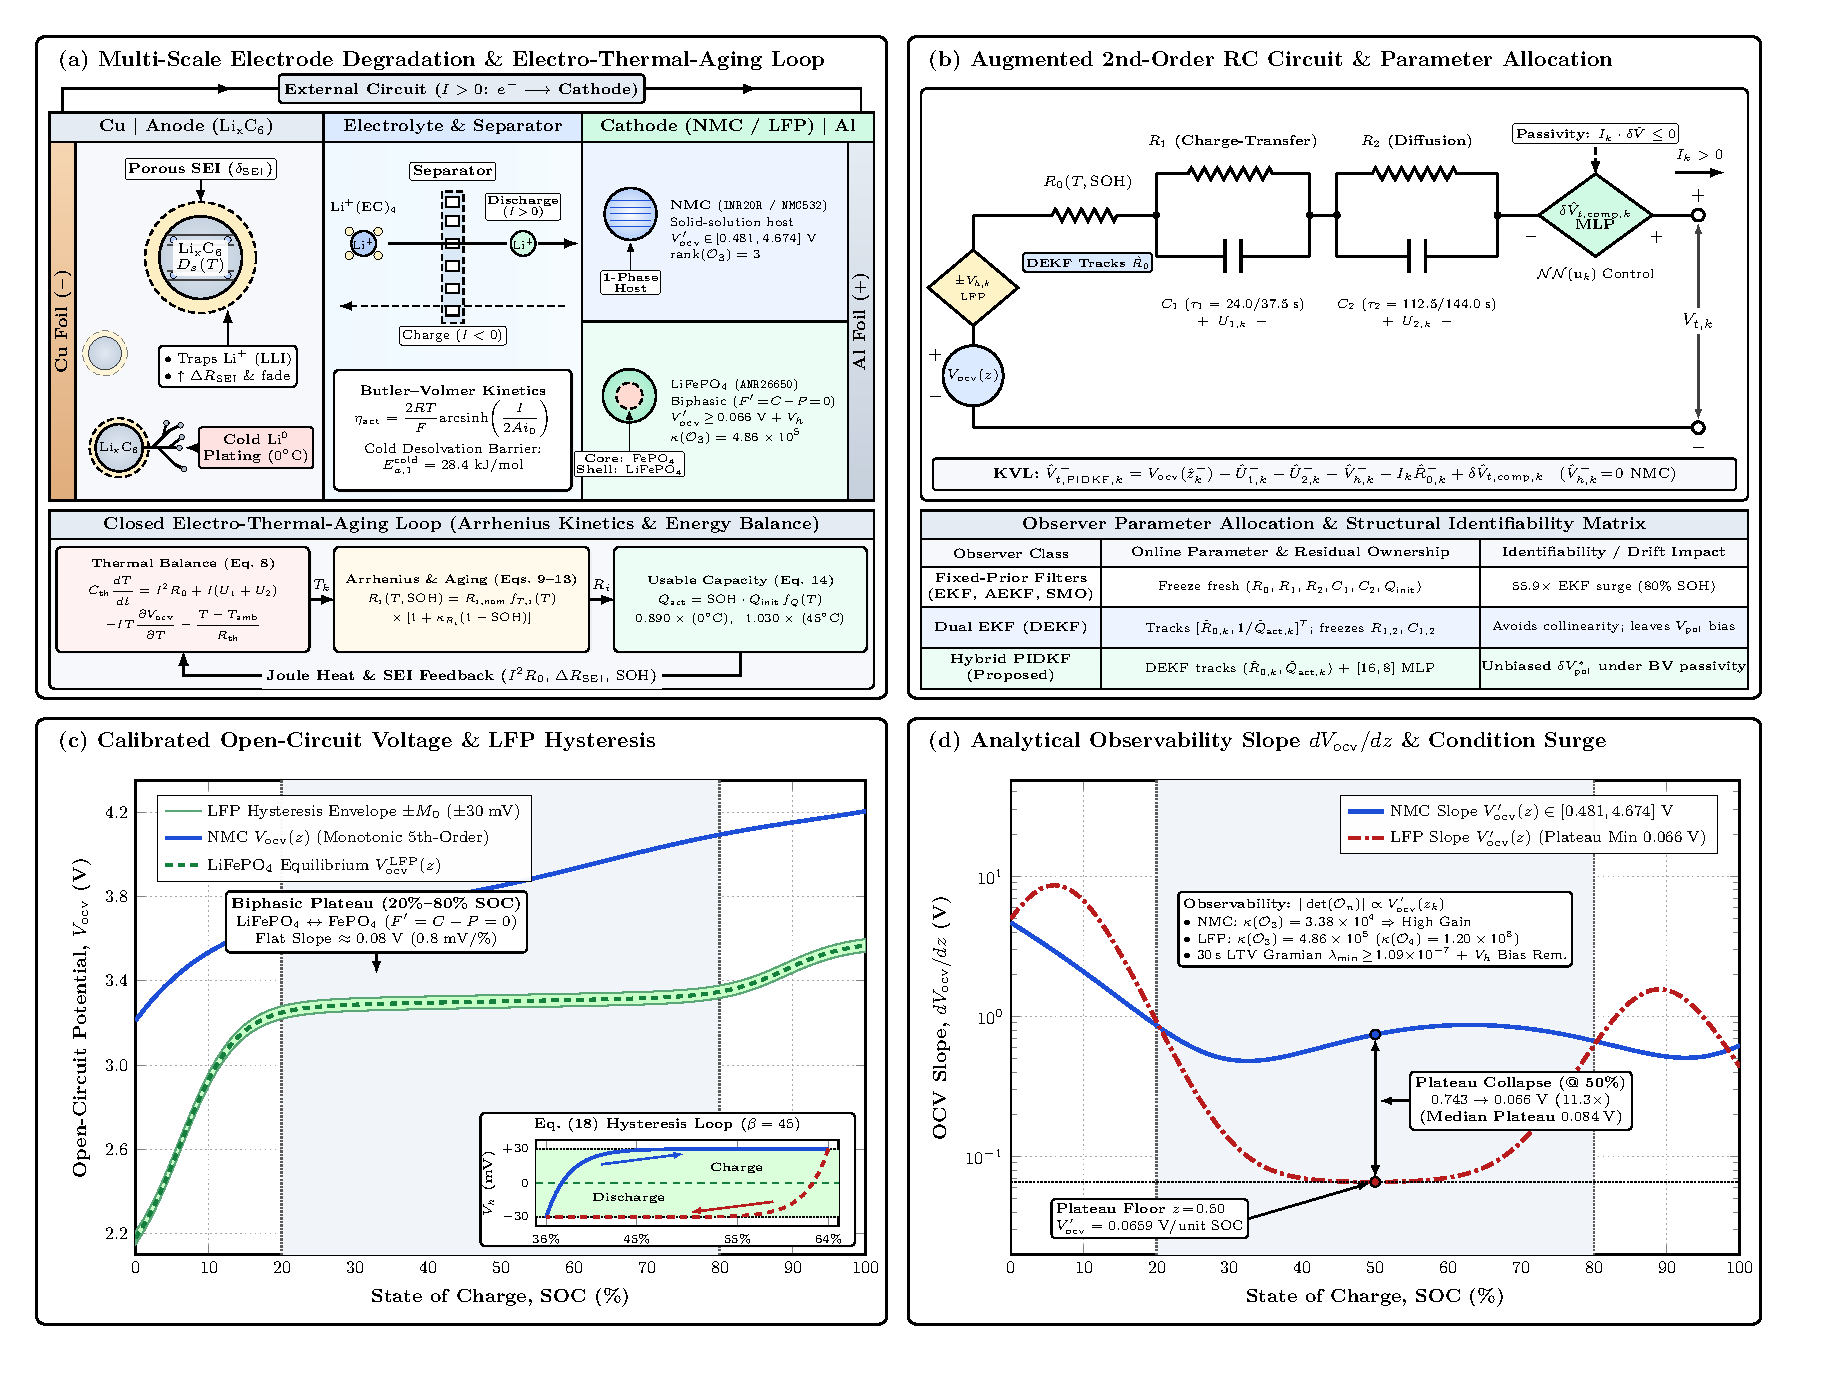
\includegraphics[width=0.98\textwidth]{fig1.pdf}
\caption{Coupled electro-thermal-aging physical mechanism and observability landscape: (a)~microscopic electrode degradation (anode SEI film growth, lithium plating risk, and cathode single-phase NMC vs.\ biphasic $\text{LiFePO}_4 \leftrightarrow \text{FePO}_4$ transition) coupled with the Arrhenius electro-thermal energy balance; (b)~augmented 2nd-order RC equivalent circuit incorporating dynamic hysteresis $V_{h,k}$ and neural overpotential residual $\delta\hat{V}_{t,\text{comp},k}$ alongside the structural parameter allocation principle; (c)~calibrated open-circuit voltage curves $V_{\text{ocv}}(\text{SOC})$ and strictly monotonic LFP hysteresis envelope; and (d)~analytical observability slope $V_{\text{ocv}}'(z) = dV_{\text{ocv}}/dz$ illustrating the $11.3$-fold plateau collapse and condition number amplification.\label{fig:0_mechanism}}
\end{figure}

%%%%%%%%%%%%%%%%%%%%%%%%%%%%%%%%%%%%%%%%%%%%%%%%%%%%%%%%%%%%%%%%%%%%%%
\section{State-of-Charge Estimation Methodologies}
This section formulates the benchmark estimators (EKF, UKF, AEKF, DEKF, SMO, BiLSTM-Attn, Unconstrained MLP, and PINN-SOC) within a unified discrete-time framework before introducing the proposed hybrid PIDKF.

\subsection{Extended Kalman Filter (EKF)}
Within the nonlinear Kalman filtering family, higher-order sigma-point variants such as UKF~\cite{Plett2006ukf,He2013ukf} propagate $2n+1$ deterministic sigma points via scaled unscented transform (UT) coefficients ($\alpha_{\text{UT}} = 10^{-3}$, $\beta_{\text{UT}} = 2$, $\kappa_{\text{UT}} = 0$) over state dimension $n \in \{3,4\}$ to avoid explicit Jacobian evaluation. Evaluated under identical constant process and measurement noise covariances ($\mathbf{Q}_k \equiv \mathbf{Q}, R_v$), UKF mirrors EKF accuracy on fresh cells while incurring more than three times the analytical ARMv7E-M compute load ($12.98\;\upmu\mathrm{s}$ vs.\ $3.69\;\upmu\mathrm{s}$; Table~\ref{tab:8_embedded}), and still diverges at comparable magnitude under severe aging ($3.772\%$ vs.\ $3.745\%$ RMSE at $80\%$ SOH) because parameter drift overwhelms quadrature refinements. Consequently, both EKF and UKF are reported in our Tier~2 benchmarks while EKF serves as the canonical fixed-parameter baseline.

Conceptually, EKF alternates between predicting the next internal state from the circuit model and correcting that prediction using the measured terminal-voltage discrepancy. At each step, EKF linearizes the terminal voltage observation model around the \emph{a priori} state estimate $\hat{\mathbf{x}}_k^-$ (with \emph{a priori} SOC component $\hat{z}_k^-$) via the observation Jacobian $\mathbf{H}_k$ (where superscripts $-$ and $+$ denote \emph{a priori} and \emph{a posteriori} quantities, respectively)~\cite{Plett2004part3}:
\begin{align}\label{eqn:ekf_jacobian}
\mathbf{H}_k^{\text{NMC}} &= \begin{bmatrix} V_{\text{ocv}}'(\hat{z}_k^-) & -1 & -1 \end{bmatrix}, \nonumber\\
\mathbf{H}_k^{\text{LFP}} &= \begin{bmatrix} V_{\text{ocv}}'(\hat{z}_k^-) & -1 & -1 & -1 \end{bmatrix},
\end{align}
where the trailing negative entry captures subtractive hysteresis overpotential in LFP cells. The recursive cycle alternates between a time-prediction stage:
\begin{align}
\hat{\mathbf{x}}_k^- &= \mathbf{A}_{k-1} \hat{\mathbf{x}}_{k-1}^+ + \mathbf{B}_{k-1} I_{k-1} + \mathbf{g}_{k-1}, \label{eqn:ekf_pred_state}\\
\mathbf{P}_k^- &= \mathbf{A}_{k-1} \mathbf{P}_{k-1}^+ \mathbf{A}_{k-1}^T + \mathbf{Q}, \label{eqn:ekf_pred_cov}
\end{align}
and a measurement-correction stage updating the state and covariance $\mathbf{P}_k^+$:
\begin{align}
e_k &= V_k - \hat{V}_{t,k}^-, \quad \mathbf{K}_k = \mathbf{P}_k^- \mathbf{H}_k^T \left( \mathbf{H}_k \mathbf{P}_k^- \mathbf{H}_k^T + R_v \right)^{-1}, \label{eqn:ekf_gain}\\
\hat{\mathbf{x}}_k^+ &= \hat{\mathbf{x}}_k^- + \mathbf{K}_k e_k, \label{eqn:ekf_upd_state}\\
\mathbf{P}_k^+ &= (\mathbf{I} - \mathbf{K}_k \mathbf{H}_k) \mathbf{P}_k^- (\mathbf{I} - \mathbf{K}_k \mathbf{H}_k)^T + \mathbf{K}_k R_v \mathbf{K}_k^T, \label{eqn:ekf_joseph}
\end{align}
where $\mathbf{P}_k^-$ and $\mathbf{P}_k^+$ denote the \emph{a priori} and \emph{a posteriori} state error covariances, $\mathbf{g}_{k-1}$ vanishes for NMC and follows Eq.~\eqref{eqn:hysteresis_discrete} for LFP, $e_k$ is the voltage innovation relative to predicted terminal voltage $\hat{V}_{t,k}^-$, and $\mathbf{K}_k$ is the Kalman gain with identity matrix $\mathbf{I}$. Equation~\eqref{eqn:ekf_joseph} implements the stabilized Joseph covariance update to guarantee matrix symmetry and positive-definiteness (denoted $\mathbf{P}_k^+ \succ 0$ in the Loewner matrix ordering) under finite-precision arithmetic.

\subsection{Adaptive Extended Kalman Filter (AEKF)}
Fixed noise covariances degrade accuracy whenever sensor noise or unmodeled polarization shifts across regimes. The AEKF augments EKF with a Sage--Husa (SH) online adaptive noise estimator~\cite{Xiang2022aekf}:
\begin{align}
\hat{r}_k &= (1 - d_k)\hat{r}_{k-1} + d_k \left( V_k - \hat{V}_{t,k}^- \right), \label{eqn:sh_mean}\\
\hat{R}_{v,k} &= (1 - d_k)\hat{R}_{v,k-1} + d_k \left( e_k^2 - \mathbf{H}_k \mathbf{P}_k^- \mathbf{H}_k^T \right), \label{eqn:sh_meas_cov}
\end{align}
where $\hat{r}_k$ is the estimated innovation bias, $\hat{R}_{v,k}$ is the adaptive scalar measurement noise variance, and $d_k$ is an exponential weighting sequence controlled by forgetting factor $\lambda_{\text{SH}}$ (Appendix~\ref{app:parameters}). Because process covariance $\mathbf{Q}$ and measurement variance $R_v$ cannot both be uniquely identified from a single scalar innovation sequence, $\mathbf{Q}$ remains fixed at its calibrated baseline while $\hat{R}_{v,k}$ is projected onto a strictly positive lower variance floor $R_{v,\min} > 0$ to preserve positive-definiteness.

\subsection{Dual Extended Kalman Filter (DEKF)}
To separate fast state dynamics from slow parameter evolution, DEKF couples two interacting Kalman filters in parallel~\cite{Plett2004part3,Charkhgard2010dekf}. A fast state filter updates $\mathbf{x}_k$ conditioned on the current parameter estimate $\hat{\boldsymbol{\theta}}_k = [\hat{R}_{0,k}, 1/\hat{Q}_{\text{act},k}]^T$, while a concurrent parameter filter models degradation as a slow random walk $\boldsymbol{\theta}_{k+1} = \boldsymbol{\theta}_k + \mathbf{w}_{\theta,k}$ driven by parameter process noise $\mathbf{w}_{\theta,k} \sim \mathcal{N}(\mathbf{0}, \mathbf{Q}_\theta)$ with covariance $\mathbf{Q}_\theta$. Accounting for lagged state sensitivity through Plett's recurrent total derivative recursion~\cite{Plett2004part3}:
\begin{equation}\label{eqn:dekf_param_jacobian}
\mathbf{C}_{\theta,k} = \left.\frac{\partial g(\hat{\mathbf{x}}_k^-, I_k, \boldsymbol{\theta})}{\partial \boldsymbol{\theta}}\right|_{\hat{\boldsymbol{\theta}}_k^-} + \mathbf{H}_k \frac{d\hat{\mathbf{x}}_k^-}{d\boldsymbol{\theta}}, \qquad
\frac{d\hat{\mathbf{x}}_k^-}{d\boldsymbol{\theta}} = \mathbf{A}_{k-1} \frac{d\hat{\mathbf{x}}_{k-1}^+}{d\boldsymbol{\theta}} + \frac{\partial \mathbf{f}}{\partial \boldsymbol{\theta}},
\end{equation}
where $\mathbf{C}_{\theta,k}$ is the total parameter observation sensitivity matrix, $g(\hat{\mathbf{x}}_k^-, I_k, \boldsymbol{\theta}) \equiv \hat{V}_{t,k}^-$ denotes the terminal voltage output map (giving $\partial g/\partial\boldsymbol{\theta} = [-I_k,\; 0]$), and $\mathbf{f}(\cdot)$ denotes the discrete state-transition map ($\partial \mathbf{f}/\partial \boldsymbol{\theta}$ isolating inverse-capacity integration along $\text{SOC}_k$), capturing how capacity shifts accumulate across multiple steps rather than a single lag. Driven by scalar parameter innovation variance $R_{\theta,v}$ and parameter covariances $\mathbf{P}_{\theta,k}^-$ and $\mathbf{P}_{\theta,k}^+$, the parameter filter updates recursively via the stabilized Joseph form (with hard rest innovation gating freezing $\mathbf{K}_k = \mathbf{0}$ and $\mathbf{K}_{\theta,k} = \mathbf{0}$ whenever $|I_k| < 10\;\mathrm{mA}$):
\begin{align}
\mathbf{K}_{\theta,k} &= \mathbf{P}_{\theta,k}^- \mathbf{C}_{\theta,k}^T [ \mathbf{C}_{\theta,k} \mathbf{P}_{\theta,k}^- \mathbf{C}_{\theta,k}^T + R_{\theta,v} ]^{-1}, \label{eqn:dekf_param_gain}\\
\hat{\boldsymbol{\theta}}_k^+ &= \hat{\boldsymbol{\theta}}_k^- + \mathbf{K}_{\theta,k} e_k, \label{eqn:dekf_param_upd}\\
\mathbf{P}_{\theta,k}^+ &= (\mathbf{I} - \mathbf{K}_{\theta,k} \mathbf{C}_{\theta,k}) \mathbf{P}_{\theta,k}^- (\mathbf{I} - \mathbf{K}_{\theta,k} \mathbf{C}_{\theta,k})^T + \mathbf{K}_{\theta,k} R_{\theta,v} \mathbf{K}_{\theta,k}^T. \label{eqn:dekf_param_cov}
\end{align}

\subsection{Sliding Mode Observer (SMO)}
The SMO enforces robustness against bounded model-plant mismatch by driving voltage tracking errors onto a boundary layer of thickness $\mu$ around the zero-voltage-error target (sliding manifold) $S_k = V_{\text{meas},k} - \hat{V}_{t,k} = 0$ for state estimate $\hat{\mathbf{x}}_k$ (with SOC coordinate $\hat{z}_k$, abbreviated $\hat{z}$), where $V_{\text{meas},k} \equiv V_k$ is the measured terminal voltage and $\hat{V}_{t,k}$ is the observer terminal voltage prediction~\cite{Chen2016smo,Huangfu2018smo}:
\begin{equation}\label{eqn:smo_state_eq}
\hat{\mathbf{x}}_{k+1} = \mathbf{A}_k \hat{\mathbf{x}}_k + \mathbf{B}_k I_k + \mathbf{g}_k + \mathbf{L}(\hat{z}_k) \operatorname{sat}\left( \frac{S_k}{\mu} \right),
\end{equation}
with continuous saturation function $\operatorname{sat}(\cdot)$ and scheduled state-feedback injection vector $\mathbf{L}(\hat{z}_k)$. To prevent gain explosion across flat plateaus while preserving reachability on steep OCV slopes, switching injection acts exclusively along the SOC coordinate:
\begin{equation}
\mathbf{L}(\hat{z}) = \left[\frac{l_{\text{smo}}}{\max(\alpha_{\min}, V_{\text{ocv}}^\prime(\hat{z}))},\, 0,\, 0,\, (0)\right]^T,
\end{equation}
where $l_{\text{smo}}$ is the scalar injection gain, $\alpha_{\min}$ is the minimum derivative regularization threshold, and the parenthesized fourth entry applies to the four-state LFP model (Appendix~\ref{app:parameters}). Whenever $V_{\text{ocv}}^\prime(\hat{z}) \ge \alpha_{\min}$, the effective manifold gain $\gamma(\hat{z}) \equiv \mathbf{H}_k\mathbf{L}(\hat{z}) = l_{\text{smo}}$ strictly exceeds the nominal disturbance bound $\Phi_d$, while setting the polarization and hysteresis coordinates of $\mathbf{L}(\hat{z}_k)$ to zero ($l_2 = l_3 = l_h = 0$) lets internal overpotentials evolve along passive dissipative dynamics without high-frequency switching chattering (discrete quasi-sliding mode proof in Appendix~\ref{app:lyapunov}).

\subsection{Bidirectional LSTM with Self-Attention (BiLSTM-Attn)}
As the data-driven sequence baseline, BiLSTM-Attn maps a causal sliding window (using only past and present telemetry) of current, voltage, and temperature measurements:
\begin{equation}
\mathbf{X}_k = [I_{k-W+1:k},\, V_{k-W+1:k},\, T_{k-W+1:k}] \in \mathbb{R}^{W \times 3},
\end{equation}
across look-back window length $W = 30\;\mathrm{s}$ (Appendix~\ref{app:parameters}) in real matrix space $\mathbb{R}^{W \times 3}$ into forward ($\overrightarrow{\mathbf{h}}_t$) and backward ($\overleftarrow{\mathbf{h}}_t$) hidden representations at window step $t \in \{1,\dots,W\}$ of dimension $D = 32$ per direction ($13,698$ total float32 parameters, $53.51\;\mathrm{KB}$ weights Flash)~\cite{Song2019bilstm,Vaswani2017attention}. Concatenating both directions (denoted $\|$) into $\mathbf{h}_t = [\overrightarrow{\mathbf{h}}_t \,\|\, \overleftarrow{\mathbf{h}}_t] \in \mathbb{R}^{2 D}$, a temporal self-attention layer computes alignment scores $u_t$ and normalized attention weights $\alpha_t$ via learnable weight matrix $\mathbf{W}_a$, bias $\mathbf{b}_a$, and projection vector $\mathbf{v}$:
\begin{align}
u_t &= \mathbf{v}^T \tanh(\mathbf{W}_a \mathbf{h}_t + \mathbf{b}_a), \quad \alpha_t = \frac{\exp(u_t)}{\sum_{j=1}^W \exp(u_j)}, \label{eqn:attn_weight}\\
\mathbf{c}_k &= \sum_{t=1}^W \alpha_t \mathbf{h}_t, \label{eqn:attn_context}
\end{align}
yielding a compact context vector $\mathbf{c}_k$ (weighting which recent time steps matter most for estimating current SOC) decoded through fully connected layers into $\hat{z}_k$.

\subsection{Physics-Informed Neural Network (PINN-SOC)}
Rather than treating SOC estimation as unconstrained regression, PINN-SOC embeds physical conservation laws directly into the neural training graph~\cite{Raissi2019pinn,Brancato2026}. To preserve strict time-shift invariance over multi-hour duty cycles, the neural network operator $\mathcal{NN}_1$ ingests strictly causal instantaneous and derivative telemetry $\mathbf{u}_k = [I_k, V_{t,k}, T_k, dV_{t,k}/dt, \hat{\text{SOH}}_{\text{latched}}]^T \in \mathbb{R}^5$ (using sampled terminal voltage $V_{t,k} \equiv V_k$ and temperature $T_k$, while omitting raw clock time $t_k$), where in blind test deployment latched health indicator $\hat{\text{SOH}}_{\text{latched}}$ remains at nominal $1.00$ without oracle aging leakage~\cite{Le2026charging}. Battery charge depletion obeys the Faradaic conservation ordinary differential equation (ODE):
\begin{equation}\label{eqn:pinn_ode}
\frac{d\,\text{SOC}(t)}{dt} = -\frac{\eta(I)\, I(t)}{3600\,Q_{\text{act}}(T, \text{SOH})}.
\end{equation}
Rather than explicit dependence on raw clock time, discrete sample differences yield $d\hat{z}/dt \approx (\hat{z}_{k+1} - \hat{z}_k)/\Delta t$ for the Faradaic residual $\mathcal{R}_{\text{Faraday},k}$, while automatic differentiation with respect to terminal voltage $\partial \hat{z}/\partial V_{t,k}$ enforces thermodynamic monotonicity:
\begin{align}
\mathcal{R}_{\text{Faraday},k} &= \frac{\hat{z}_{k+1} - \hat{z}_k}{\Delta t} + \frac{\eta(I_k)\, I_k}{3600\,Q_{\text{nom}} \hat{\text{SOH}}_{\text{latched},k}}, \label{eqn:res_faraday}
\end{align}
where $Q_{\text{nom}} \equiv Q_{\text{init}}$ is the nominal fresh capacity and online inference remains strictly causal at each $1\;\mathrm{s}$ step.

Simultaneously, because internal polarization and hysteresis voltages ($\hat{V}_{\text{pol}} \equiv \hat{U}_1 + \hat{U}_2 + \hat{V}_h$) cannot be measured directly in field packs, PINN-SOC enforces terminal-voltage Kirchhoff consistency across the residual manifold:
\begin{equation}\label{eqn:res_kvl}
\mathcal{R}_{\text{KVL}}(t) = V_{\text{meas}}(t) - \left[ V_{\text{ocv}}(\hat{z}(t)) - I(t) R_0 - \hat{V}_{\text{pol}}(t) \right],
\end{equation}
while an output Sigmoid activation guarantees bounded estimates $\hat{z} \in (0, 1)$. During offline optimization over parameters $\boldsymbol{\theta}_{\text{PINN}}$ ($6,690$ float32 parameters, $26.13\;\mathrm{KB}$ Flash), supervised data loss $\mathcal{L}_{\text{data}}$ across $N_d$ labeled samples (with reference state $\text{SOC}_k^{\text{ref}}$) is balanced against physics residuals ($\mathcal{L}_{\text{Faraday}}, \mathcal{L}_{\text{KVL}}, \mathcal{L}_{\text{mono}}$) weighted by coefficients $\lambda_{\text{Faraday}}, \lambda_{\text{KVL}}, \lambda_{\text{mono}}$ over $N_c$ collocation timestamps $t_j$ ($j \in \{1,\dots,N_c\}$, with collocation estimates $\hat{z}_j \equiv \hat{z}(t_j)$ and voltages $V_{t,j} \equiv V_t(t_j)$):
\begin{equation}\label{eqn:pinn_loss}
\mathcal{L}_{\text{total}}(\boldsymbol{\theta}_{\text{PINN}}) = \mathcal{L}_{\text{data}} + \lambda_{\text{Faraday}} \mathcal{L}_{\text{Faraday}} + \lambda_{\text{KVL}} \mathcal{L}_{\text{KVL}} + \lambda_{\text{mono}} \mathcal{L}_{\text{mono}},
\end{equation}
where individual components enforce data fidelity, differential charge conservation, algebraic voltage consistency, and quasi-stationary monotonicity ($\partial \hat{z}/\partial V_t \ge 0$, ensuring estimated SOC rises whenever voltage rises):
\begin{align}
\mathcal{L}_{\text{data}} &= \frac{1}{N_d} \sum_{k=1}^{N_d} (\hat{z}_k - \text{SOC}_k^{\text{ref}})^2, \quad \mathcal{L}_{\text{Faraday}} = \frac{1}{N_c} \sum_{j=1}^{N_c} \|\mathcal{R}_{\text{Faraday}}(t_j)\|^2, \label{eqn:pinn_loss_data_faraday} \\
\mathcal{L}_{\text{KVL}} &= \frac{1}{N_c} \sum_{j=1}^{N_c} \|\mathcal{R}_{\text{KVL}}(t_j)\|^2, \quad \mathcal{L}_{\text{mono}} = \frac{1}{N_c}\sum_{j=1}^{N_c} \left[\max\left(0, -\frac{\partial \hat{z}_j}{\partial V_{t,j}}\right)\right]^2. \label{eqn:pinn_loss_kvl_mono}
\end{align}
Trained as a four-layer MLP with Gaussian Error Linear Unit (GELU) activations via decoupled weight-decay Adaptive Moment Estimation (AdamW; hyperparameters in Appendix~\ref{app:parameters}), under strictly blind nominal-prior deployment without online parameter tracking the soft KVL and Faraday penalties trade data-fit flexibility against fixed-parameter stiffness relative to an unconstrained MLP ($3.625\pm0.851\%$ vs.\ $3.201\pm0.518\%$, Table~\ref{tab:1_udds}), directly motivating recursive state--parameter fusion in PIDKF.

\subsection{Proposed Hybrid Architecture: PIDKF}\label{sec:pidkf}
\emph{Backbone, Resistance Conditioning, and Passivity Saturation.} To unite the recursive convergence guarantees and parameter adaptability of DEKF with the nonlinear representational capacity of physics-constrained neural networks, we introduce the hybrid \textbf{PIDKF} (Fig.~\ref{fig:0_framework}). In this architecture, a DEKF backbone tracks both state $\hat{\mathbf{x}}_k$ (3-state for NMC and 4-state including dynamic hysteresis $\hat{V}_{h,k}$ via Eq.~\eqref{eqn:vt_lfp} for LFP) and parameters $\hat{\boldsymbol{\theta}}_k = [\hat{R}_{0,k}, 1/\hat{Q}_{\text{act},k}]^T$ initialized strictly from fresh room-temperature nominal priors ($100\%$ SOH, $25^\circ\text{C}$), while a compact feedforward compensator $\mathcal{NN}(\mathbf{u}_k; \boldsymbol{\theta}_{\text{net}})$ parameterized by trainable weight vector $\boldsymbol{\theta}_{\text{net}}$ predicts unmodeled kinetic and diffusion polarization residuals $\delta\hat{V}_{t,\text{comp},k}$ from online measurements and \emph{a priori} states:
\begin{equation}\label{eqn:pidkf_input}
\mathbf{u}_k = \left[I_k,\; T_k,\; \hat{z}_k^-,\; \hat{U}_{1,k}^-,\; \hat{U}_{2,k}^-,\; \hat{R}_{0,k}^-\right]^T \in \mathbb{R}^6.
\end{equation}
Conditioning on the fast-converging online series resistance $\hat{R}_{0,k}^-$ (characteristic convergence time constant $\tau_R \approx 10\text{--}30\;\mathrm{s}$) rather than slow inverse capacity $1/\hat{Q}_{\text{act},k}$ ($>2,000\;\mathrm{s}$ from uncalibrated fresh priors) eliminates oracle health leakage and provides rapid sensitivity to coupled thermal-aging impedance shifts. To prevent unphysical overpotential predictions, the neural output passes through a symmetric saturation operator bounded by a saturated Butler--Volmer current envelope $V_{\text{pol}}^{\max}(I_k) = \kappa_0 + \kappa_1 \min(|I_k|, I_{\max})$ (with $\kappa_0 = 15\;\mathrm{mV}$, $\kappa_1 = 22\;\mathrm{m}\Omega$, and $I_{\max} = 6.0\;\mathrm{A}$, bounding $|V_{\text{pol}}^{\max}| \le 147\;\mathrm{mV}$) followed by hard dissipative passivity projection setting $\delta\hat{V}_{t,\text{comp},k} = 0$ whenever $I_k \cdot \delta\hat{V}_{t,\text{comp},k} > 0$ outside the $10\;\mathrm{mA}$ rest threshold.

\emph{Causal Residual Calibration.} Strict causality separates offline calibration from online embedded inference. During offline training on Cell Batch~A DST trajectories, target voltage residuals $\delta V_{t,\text{target},k}$ capture true plant terminal voltage minus fixed-RC 2-RC predictions driven by forward Batch~A ground truth and causal prior estimates, preventing test-set or future leakage. During online BMS operation, adding $\delta\hat{V}_{t,\text{comp},k}$ to the ECM terminal voltage prediction forms the PIDKF voltage innovation $e_{k,\text{PIDKF}}$ driving both state and parameter updates, while inflated effective innovation variances $R_{\text{eff},k} \equiv R_{\text{eff}} = R_v + \sigma_{\text{NN}}^2 + \sigma_{\text{approx}}^2 = 1.068 \times 10^{-3}\;\mathrm{V}^2$ and $R_{\theta,\text{eff}} = R_{\theta,v} + \sigma_{\text{NN}}^2 = 1.0064 \times 10^{-2}\;\mathrm{V}^2$ (where $\sigma_{\text{NN}} = 8.0\;\mathrm{mV}$ and $\sigma_{\text{approx}} = 2.0\;\mathrm{mV}$ denote neural residual and Jacobian decoupling standard deviations) preserve consistent Kalman weighting.

\emph{Exogenous Sensitivity Decoupling.} Exact differentiation of $\delta\hat{V} \equiv \delta\hat{V}_{t,\text{comp},k}$ through the composite observation model (with factor $15\;\mathrm{V}^{-1}$ reflecting polarization input normalization) adds neural chain-rule Jacobian entries $\mathbf{J}_{\text{NN},k}$ to $\mathbf{H}_k$ to yield the exact Jacobians $\mathbf{H}_{\text{PIDKF},k}^{\text{exact}}$ and $\mathbf{C}_{\theta,\text{PIDKF},k}^{\text{exact}}$:
\begin{align*}
\mathbf{J}_{\text{NN},k} &= \left[\frac{\partial\delta\hat{V}}{\partial\hat{z}_k^-},\; 15\frac{\partial\delta\hat{V}}{\partial\hat{U}_{1,k}^-},\; 15\frac{\partial\delta\hat{V}}{\partial\hat{U}_{2,k}^-},\; (0)\right], \qquad
\mathbf{H}_{\text{PIDKF},k}^{\text{exact}} = \mathbf{H}_k + \mathbf{J}_{\text{NN},k}, \\
\mathbf{C}_{\theta,\text{PIDKF},k}^{\text{exact}} &= \mathbf{C}_{\theta,k} + \mathbf{J}_{\text{NN},k}\frac{d\hat{\mathbf{x}}_k^-}{d\boldsymbol{\theta}} + \left[\frac{\partial \delta\hat{V}}{\partial \hat{R}_{0,k}^-},\; 0\right].
\end{align*}
{\sloppy Over aged NMC UDDS operation (Phase~10), automatic differentiation shows $\|\mathbf{J}_{\text{NN},k}\|_2 / \|\mathbf{H}_k\|_2$ averages $16.8\%$ (peak $28.7\%$) with sign reversals near clamping and activation knees. Injecting non-smooth neural derivatives directly into the Kalman gain $\mathbf{K}_k$ destabilizes state-parameter covariance contraction ($1.894\pm0.495\%$ RMSE on $85\%$ SOH NMC and $1.033\pm0.468\%$ on LFP). PIDKF therefore adopts \emph{exogenous sensitivity decoupling} ($\mathbf{H}_{\text{PIDKF},k} \approx \mathbf{H}_k$ and $\mathbf{C}_{\theta,\text{PIDKF},k} \approx \mathbf{C}_{\theta,k}$), absorbing the bounded approximation difference inside $\sigma_{\text{approx}}^2$: this shields $\mathbf{K}_k$ from neural gradient noise, slashing aged $85\%$ SOH RMSE to $0.554\pm0.018\%$ (NMC) and $0.593\pm0.048\%$ (LFP) while removing backpropagation overhead from MCU execution.\par}

\emph{Physics-Constrained Training Objective.} Rather than enforcing continuous ODE collocation during deployment, the neural compensator acts as a Butler--Volmer-constrained overpotential surrogate trained over $N$ samples via composite objective $\mathcal{L}_{\text{PIDKF}}$ combining residual mean-square error $\mathcal{L}_{\text{res}} = \frac{1}{N}\sum_{k=1}^N (\delta\hat{V}_{t,\text{comp},k} - \delta V_{t,\text{target},k})^2$, physics penalty $\mathcal{L}_{\text{phys}}$ weighted by $\lambda_{\text{phys}} = 0.50$ (with passivity multiplier $\gamma_I = 1.0$), and Euclidean $L_2$ weight decay weighted by $\lambda_{\text{reg}} = 10^{-5}$:
\begin{align}
\mathcal{L}_{\text{PIDKF}}(\boldsymbol{\theta}_{\text{net}}) &= \mathcal{L}_{\text{res}} + \lambda_{\text{phys}} \mathcal{L}_{\text{phys}} + \lambda_{\text{reg}} \|\boldsymbol{\theta}_{\text{net}}\|_2^2, \label{eqn:loss_pidkf}\\
\mathcal{L}_{\text{phys}} &= \frac{1}{N}\sum_{k=1}^N \left[\max\left(0, |\delta \hat{V}_{t,\text{comp},k}| - V_{\text{pol}}^{\max}\right)^2 + \gamma_I \max\left(0, I_k \delta \hat{V}_{t,\text{comp},k}\right)^2\right], \label{eqn:loss_pidkf_phys}
\end{align}
yielding a compact $[6 \rightarrow 16 \rightarrow 8 \rightarrow 1]$ GELU MLP containing strictly $257$ float32 parameters ($1.00\;\mathrm{KB} = 1,028\;\mathrm{B}$ weights Flash; $580$ compensator floating-point operations [FLOPs] per step, $1,540$ total PIDKF FLOPs/step; Table~\ref{tab:8_embedded}).

\emph{Closed-Loop ISS and UUB Stability.} Closed-loop ISS and UUB convergence of PIDKF follow from two structural properties formalized in Appendix~\ref{app:parameters}. First, hard overpotential clipping (upper bound $\bar{V}^*$) together with bounded plant polarization residuals and bounded parameter estimation error $\|\tilde{\boldsymbol{\theta}}_k\| \le \bar{\theta}$ (inducing voltage deviation bound $\bar{\delta}_\theta$, where $\tilde{\boldsymbol{\theta}}_k \equiv \boldsymbol{\theta}_k - \hat{\boldsymbol{\theta}}_k$) ensures total unmodeled voltage perturbation $\varepsilon_k$ stays bounded by $\bar{\varepsilon}_{\text{tot}} \equiv \bar{V}^* + \kappa_0 + \kappa_1 I_{\max} + \bar{\delta}_\theta$. Second, active drive windows of length $N$ satisfying Uniform Complete Observability (UCO) and Uniform Complete Controllability (UCC) alternate with rest intervals $T_{\text{rest},m} \le T_{\max}$, during which rest gating ($|I_k| < 10\;\mathrm{mA}$) freezes $\mathbf{K}_k = \mathbf{0}, \mathbf{K}_{\theta,k} = \mathbf{0}$ so that closed-loop error transition matrix $\mathbf{F}_k \equiv \mathbf{A}_k(\mathbf{I} - \mathbf{K}_k\mathbf{H}_k)$ stays non-expansive under uniform process and measurement noise bounds ($\underline{q}, \bar{q}, \underline{r}, \bar{r}$). Under assumptions (A1)--(A4) detailed in Appendix~\ref{app:parameters} (with uniform bounds $\|\mathbf{A}_k\|_2 \le \bar{A}$ and $\|\mathbf{K}_k\|_2 \le \bar{K}$), multi-cycle transition products $\boldsymbol{\Phi}_F$ contract geometrically with rate $\rho < 1$, prefactor $c \ge 1$, and uniform Riccati bounds $\underline{p}\mathbf{I} \preceq \mathbf{P}_k^- \preceq \bar{p}\mathbf{I}$ (where $\preceq$ denotes Loewner matrix inequality), yielding first-moment and mean-square convergence bounds on the \emph{a priori} state error $\mathbf{e}_k^- \equiv \mathbf{x}_k - \hat{\mathbf{x}}_k^-$ (with expectation operator $\mathbb{E}[\cdot]$ and limit superior $\limsup$):
\begin{align}
\limsup_{k \to \infty} \|\mathbb{E}[\mathbf{e}_k^-]\| &\le \frac{c \bar{A} \bar{K} \bar{\varepsilon}_{\text{tot}}}{1 - \rho} < \infty, \label{eqn:bibs_pidkf}\\
\limsup_{k \to \infty} \mathbb{E}[\|\mathbf{e}_k^-\|^2] &\le n\bar{p} + 2\sqrt{n\bar{p}}\left(\frac{c \bar{A} \bar{K} \bar{\varepsilon}_{\text{tot}}}{1 - \rho}\right) + \left(\frac{c \bar{A} \bar{K} \bar{\varepsilon}_{\text{tot}}}{1 - \rho}\right)^2 < \infty, \label{eqn:ms_pidkf}
\end{align}
preserving local exponential contraction of initialization offsets under intermittent rest and bounded parameter drift~\cite{Reif1999ekf}.

\begin{figure}[htbp]
\centering
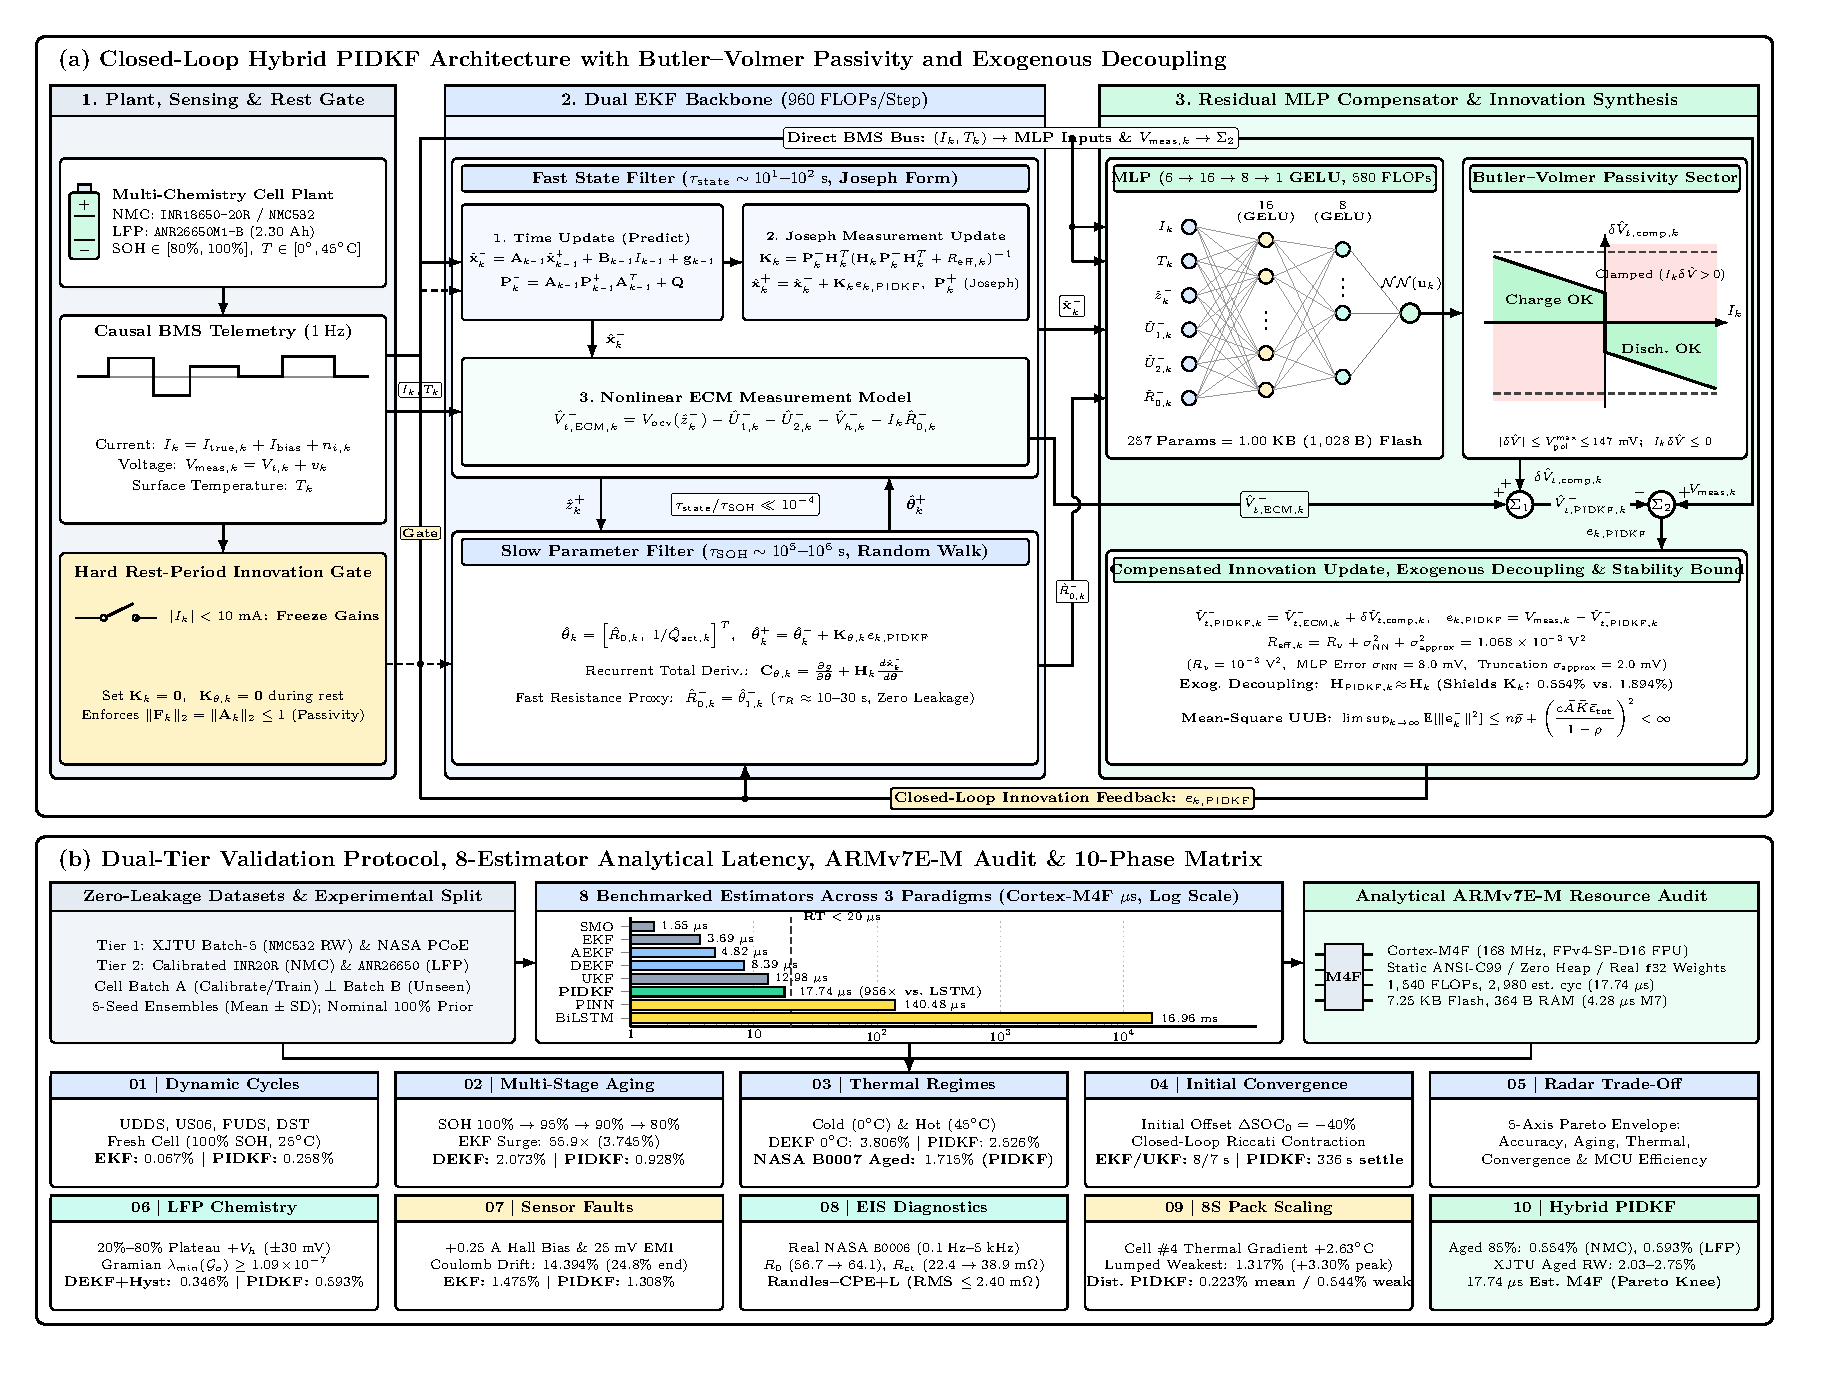
\includegraphics[width=0.98\textwidth]{fig2.pdf}
\caption{Proposed hybrid PIDKF architecture and 10-phase benchmarking framework: (a)~closed-loop interaction between the Dual EKF backbone, fast online $\hat{R}_{0,k}^-$ conditioning, the $257$-parameter $[6\to 16\to 8\to 1]$ neural compensator, dissipative Butler--Volmer passivity projection ($I_k \cdot \delta\hat{V}_{t,\text{comp},k} \le 0$), and exogenous Jacobian decoupling; and (b)~dual-tier experimental/co-simulation validation split, 8-estimator analytical ARMv7E-M latency profiling, static ANSI-C99 resource audit, and 10 evaluation phases.\label{fig:0_framework}}
\end{figure}
%%%%%%%%%%%%%%%%%%%%%%%%%%%%%%%%%%%%%%%%%%%%%%%%%%%%%%%%%%%%%%%%%%%%%%
\section{Experimental Benchmarking Platform and Methodology\label{sec:exp_setup}}
This section delineates the dual-tier validation architecture separating Tier~1 public laboratory cycler measurements from Tier~2 calibrated co-simulation, summarizes the automotive driving profiles, and defines quantitative accuracy, convergence, and aging-sensitivity metrics.

\subsection{Dual-Tier Benchmark Architecture and Data Provenance}
To avoid extrapolating from a single cell or synthetic simulator alone, we enforce an explicit two-tier validation separation:
\begin{itemize}
\item \textbf{Tier~1 Public Laboratory Cycler Validation:} Direct execution on held-out experimental measurements from two open-access repositories on disk. First, the \textbf{XJTU Batch-5} dataset~\cite{Wang2024xjtu} provides long-term $1\text{--}3\text{C}$ charge and dynamic RW discharge tests ($-2\text{ A}$ to $-7\text{ A}$ multi-amplitude pulse trains) on $2.00\;\mathrm{Ah}$ LISHEN $\text{LiNi}_{0.5}\text{Co}_{0.2}\text{Mn}_{0.3}\text{O}_2$ (NMC532) $18650$ cylindrical cells (\texttt{RW\_battery-1} and \texttt{RW\_battery-2} form strictly disjoint \emph{Batch~A} for 2-RC calibration [$R_0 = 32.0\;\mathrm{m}\Omega$, $R_1 = 7.8\;\mathrm{m}\Omega$, $R_2 = 11.0\;\mathrm{m}\Omega$, $Q_{\text{init}} = 1.865\;\mathrm{Ah}$ from $1\text{C}$ reference performance test (RPT), $39.45\;\mathrm{mV}$ fit RMS] and neural training; unseen \texttt{RW\_battery-3} and \texttt{RW\_battery-4} serve as held-out \emph{Batch~B} test cells at fresh [$100\%$] and degraded [$\sim 86.0\text{--}86.8\%$ SOH] RPT checkpoints). Second, the \textbf{NASA Ames PCoE} repository~\cite{Saha2007nasa} provides commercial $2.00\;\mathrm{Ah}$ $\text{LiCoO}_2$ $18650$ aging and extreme-temperature datasets: nominal room-temperature ECM calibration uses \texttt{B0005} cycle~0 anchored at $R_0 = 44.67\;\mathrm{m}\Omega$ strictly from fresh \texttt{B0005} EIS ($15.81\;\mathrm{mV}$ constant-current [CC] fit RMS), while real Randles--CPE+inductance impedance spectroscopy is fitted directly to $39$-frequency ($0.1\;\mathrm{Hz}\text{--}5\;\mathrm{kHz}$) spectra from \texttt{B0006} (Phase~8) and unseen test cells \texttt{B0007} ($24^\circ\text{C}$ fresh and $81\%$ aged), \texttt{B0030} ($43^\circ\text{C}$ hot, $4\text{ A}$), and \texttt{B0055/B0056} ($4^\circ\text{C}$ cold, $2\text{ A}$) quantify real-world thermal/aging generalization (Table~\ref{tab:10_tier1}). Note that raw Center for Advanced Life Cycle Engineering (CALCE) or Oxford cycler files are not claimed as Tier~1 evidence; rather, literature parameterizations of Samsung INR18650-20R (NMC, $2.00\;\mathrm{Ah}$) and A123 ANR26650M1-B (LFP, $2.30\;\mathrm{Ah}$) dynamics~\cite{He2011ecm,Hu2012ecm,Birkl2017diagnostics,Pecht2011calce} anchor the Tier~2 testbed below.
\item \textbf{Tier~2 Calibrated Co-Simulation Testbed:} Evaluates Phases~1--7 and 9--10 under controlled electro-thermal-aging ground truth across NMC and LFP plants (Table~\ref{tab:ecm_params}) with zero oracle leakage: every model-based observer (EKF, AEKF, UKF, DEKF, SMO, PIDKF) initializes strictly at nominal $100\%$ SOH and $25^\circ\text{C}$. All data-driven networks (BiLSTM-Attn, PINN-SOC, Unconstrained MLP, PIDKF compensator) train strictly on synthetic \emph{Batch~A DST} trajectories ($100\%, 90\%, 80\%$ SOH) across $5$ random seeds ($42\text{--}46$) and are evaluated strictly on unseen \emph{Batch~B UDDS, FUDS, and US06} schedules, reporting mean plus/minus one standard deviation ($\text{Mean}\pm\text{SD}$). Embedded footprint and latency metrics (Table~\ref{tab:8_embedded}) reflect exact static ANSI-C99 \texttt{struct}/\texttt{float32} weight sizing (\texttt{embedded\_c/}) and instruction-level ARMv7E-M (Cortex-M4F @ $168\;\mathrm{MHz}$ / Cortex-M7 @ $480\;\mathrm{MHz}$) FLOP/cycle accounting without unverified hardware timer claims.
\end{itemize}

\subsection{Standardized Automotive Dynamic Stress Cycles}
Four automotive duty cycles probe distinct electrochemical excitation bandwidths. Urban stop-and-go driving with frequent regenerative braking is captured by UDDS (concatenated to $3600\text{ s}$) and multi-rate FUDS profiles, which serve as the primary testbeds. Aggressive highway acceleration featuring sustained high-rate pulses up to $4\text{C}$ ($600\text{ s}$) is represented by US06, while United States Advanced Battery Consortium (USABC) step-wise DST pulses provide standardized multi-amplitude validation.

\subsection{Quantitative Performance Indices}
Algorithmic fidelity is quantified over $N$ samples relative to reference trajectory $\text{SOC}_k^{\text{true}}$ using RMSE, mean absolute error (MAE), maximum absolute error (MaxE), and first-entry reach time ($t_{\text{reach}}^{(2\%)}$) into the $2.0\%$ tolerance band from large initialization offsets ($\Delta\text{SOC}_0 = -40\%$):
\begin{align}
\text{RMSE} &= \sqrt{\tfrac{1}{N}\textstyle\sum_{k=1}^N (\text{SOC}_k^{\text{true}} - \hat{z}_k)^2} \times 100\%, \label{eqn:rmse}\\
\text{MAE} &= \tfrac{1}{N}\textstyle\sum_{k=1}^N |\text{SOC}_k^{\text{true}} - \hat{z}_k| \times 100\%, \label{eqn:mae}\\
\text{MaxE} &= \max_{1 \le k \le N} |\text{SOC}_k^{\text{true}} - \hat{z}_k| \times 100\%, \label{eqn:maxe}\\
t_{\text{reach}}^{(2\%)} &= \min\left\{ t \ge 0 \mid |\text{SOC}_t^{\text{true}} - \hat{z}_t| \le 2.0\% \right\}. \label{eqn:treach}
\end{align}
Complementing first-entry reach time, permanent settling time $t_{\text{settle}}^{(5\%)}$ records the earliest time after which tracking remains continuously within the $5.0\%$ operational corridor through evaluation horizon $T_{\text{eval}}$, while peak post-convergence error $\text{MaxE}_{\text{dyn}}$ captures the worst-case transient excursion following $t_{\text{reach}}^{(2\%)}$. Finally, degradation robustness across aging is summarized by the \textbf{Aging Sensitivity Factor} ($\text{ASF}$), which measures the percentage RMSE growth from fresh ($100\%$) to aged ($80\%$) SOH:
\begin{equation}\label{eqn:asf}
\text{ASF} = \frac{\text{RMSE}(\text{SOH}=80\%) - \text{RMSE}(\text{SOH}=100\%)}{\text{RMSE}(\text{SOH}=100\%)} \times 100\%.
\end{equation}

\section{Results and Discussion Across 10 Operational Phases}
This section presents the comparative evaluation across the ten operational stress phases introduced in Section~1, progressing from nominal tracking and capacity fade to cross-chemistry observability, pack scaling, analytical ARMv7E-M embedded resource sizing, and direct Tier~1 laboratory cycler validation.

\subsection{Phase 1: Dynamic Drive Cycle Tracking at Nominal Condition}
Table~\ref{tab:1_udds} and Fig.~\ref{fig:udds} present benchmarked tracking performance across an unseen $60\text{-min}$ concatenated UDDS schedule on a fresh NMC cell ($100\%$ SOH) at $25^\circ\text{C}$.

Under nominal fresh-cell conditions with accurately calibrated priors, Kalman-family observers outperform standalone deep learning baselines by more than an order of magnitude (Table~\ref{tab:1_udds}, Fig.~\ref{fig:udds}). Classical EKF and UKF attain virtually identical nominal precision ($0.067\%$ vs.\ $0.069\%$ RMSE), DEKF tracks cleanly at $0.073\%$ RMSE, and AEKF achieves the tightest peak transient bound ($0.432\%$ MaxE) while incurring minor steady-state overhead ($0.161\%$ RMSE) from Sage--Husa covariance adaptation. Meanwhile, PIDKF attains $0.258\pm0.111\%$ RMSE and $0.538\%$ MaxE (accepting a modest fresh-cell residual bias from its inflated innovation variance $R_{\text{eff},k}$ in exchange for strong aging and thermal generalization in Phases~2--3), while SMO reflects its $20\text{ mV}$ switching boundary layer ($1.222\%$ RMSE) and standalone neural models plateau at $3.201\text{--}4.250\%$ RMSE. Analytical ARMv7E-M MCU execution sizing across Cortex-M cores is detailed in Section~\ref{sec:hw_profiling} and Table~\ref{tab:8_embedded}.

\begin{table}[htbp]
\caption{Nominal UDDS benchmark [Tier~2 Calibrated Co-Simulation] ($25^\circ\text{C}$, $100\%$ SOH; $5$-seed Mean$\pm$SD for neural models). Analytical ARMv7E-M execution sizing is reported in Table~\ref{tab:8_embedded}.\label{tab:1_udds}}
\centering{%
\small\renewcommand{\arraystretch}{1.25}
\begin{tabular*}{\linewidth}{@{\extracolsep{\fill}}lccc}
\toprule
Algorithm & RMSE (\%) & MAE (\%) & MaxE (\%) \\
\midrule
EKF & \textbf{0.067} & \textbf{0.049} & 0.556 \\
AEKF & 0.161 & 0.130 & \textbf{0.432} \\
UKF & 0.069 & 0.055 & 0.572 \\
DEKF & 0.073 & 0.052 & 0.531 \\
SMO & 1.222 & 0.975 & 4.527 \\
BiLSTM-Attn & $4.250\pm0.653$ & 3.595 & 9.632 \\
PINN-SOC & $3.625\pm0.851$ & 3.098 & 8.744 \\
MLP (Unconstrained) & $3.201\pm0.518$ & 2.649 & 8.625 \\
PIDKF (Proposed) & $0.258\pm0.111$ & 0.240 & 0.538 \\
\bottomrule
\end{tabular*}
}%
\end{table}

\begin{figure}[htbp]
\centering
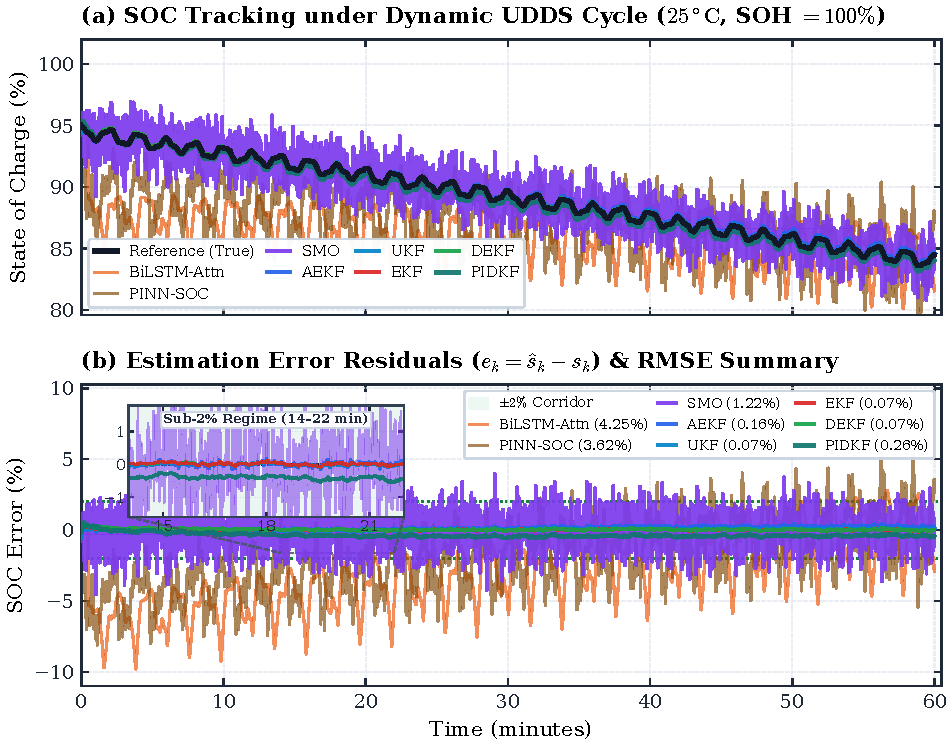
\includegraphics[width=0.88\linewidth]{fig3.pdf}
\caption{Dynamic SOC tracking and residual error comparison across benchmarked observers, neural baselines, and PIDKF under an unseen $60\text{-min}$ concatenated UDDS schedule ($3600\text{ s}$) at $25^\circ\text{C}$ and $100\%$ SOH.\label{fig:udds}}
\end{figure}

\subsection[Phase 2: Progressive Aging Degradation]{Phase 2: Progressive Aging Degradation ($100\% \rightarrow 80\%$ SOH)}
Figure~\ref{fig:aging} and Table~\ref{tab:2_aging} present the central degradation finding under strictly blind fresh initialization: the catastrophic divergence of fixed-parameter observers versus dual parameter adaptation and hybrid compensation.

As capacity fades from $100\%$ to $80\%$ SOH, fixed-parameter EKF and UKF suffer \textbf{55.9-fold} and \textbf{54.7-fold} RMSE escalations ($0.067\% \rightarrow 3.745\%$ and $0.069\% \rightarrow 3.772\%$), respectively, while AEKF degrades even further to $6.020\%$ RMSE because Sage--Husa innovation inflation cannot separate parameter drift from measurement noise (Table~\ref{tab:2_aging}, Fig.~\ref{fig:aging}). Uncompensated observers misattribute aging-induced ohmic and polarization voltage drops to thermodynamic OCV shifts, inducing persistent state bias.

Conversely, online co-estimation of $\hat{R}_{0,k}$ and $1/\hat{Q}_{\text{act},k}$ cuts aged $80\%$ SOH error nearly in half with DEKF ($2.073\%$), leaving an unmodeled polarization lag because $R_1$ grows by $150\%$ with aging while remaining frozen inside DEKF. Augmenting DEKF with the Butler--Volmer-constrained neural compensator enables \textbf{PIDKF} to absorb that polarization mismatch, uniquely holding severely aged $80\%$ SOH RMSE below $1\%$ ($0.928\pm0.027\%$). Standalone neural models show lower relative ASF simply because their fresh baselines already sit high ($3.201\text{--}4.250\%$) and remain locked at $4.118\text{--}5.026\%$ at $80\%$ SOH.

\begin{table}[htbp]
\caption{Degradation benchmark across progressive SOH stages on unseen UDDS [Tier~2 Calibrated Co-Simulation, zero oracle aging leakage, $5$-seed Mean$\pm$SD at $80\%$ SOH for neural models].\label{tab:2_aging}}
\centering{%
\small\renewcommand{\arraystretch}{1.25}%
\setlength{\tabcolsep}{2.5pt}
\begin{tabular*}{\linewidth}{@{\extracolsep{\fill}}lcccccc}
\toprule
Algorithm & SOH 100\% & SOH 95\% & SOH 90\% & SOH 85\% & SOH 80\% & ASF$^\dagger$ (\%) \\
\midrule
EKF & \textbf{0.067\%} & 0.701\% & 1.534\% & 2.578\% & 3.745\% & +5489.6\% \\
AEKF & 0.161\% & 0.760\% & 1.963\% & 3.847\% & 6.020\% & +3639.1\% \\
UKF & 0.069\% & 0.712\% & 1.555\% & 2.609\% & 3.772\% & +5366.7\% \\
DEKF & 0.073\% & 0.503\% & 1.012\% & 1.576\% & 2.073\% & +2739.7\% \\
SMO & 1.222\% & 2.046\% & 3.315\% & 4.575\% & 5.805\% & +375.0\% \\
BiLSTM-Attn & 4.250\% & 4.185\% & 4.152\% & 4.150\% & $4.193\pm0.558\%$ & $-1.3\%$ \\
PINN-SOC & 3.625\% & 3.800\% & 4.102\% & 4.508\% & $5.026\pm0.766\%$ & +38.6\% \\
MLP (Unconstrained) & 3.201\% & 3.247\% & 3.418\% & 3.707\% & $4.118\pm0.257\%$ & +28.6\% \\
\textbf{PIDKF (Proposed)} & 0.258\% & \textbf{0.372\%} & \textbf{0.515\%} & \textbf{0.772\%} & \textbf{0.928$\pm$0.027\%} & +259.7\% \\
\bottomrule
\end{tabular*}%
\vspace{2pt}
{\raggedright\scriptsize $^\dagger$ASF measures relative percentage RMSE escalation over each method's own $100\%$ SOH baseline; standalone neural baselines show low ASF only because their nominal $100\%$ SOH errors already start high ($3.201\text{--}4.250\%$).\par}
}%
\end{table}

\begin{figure}[htbp]
\centering
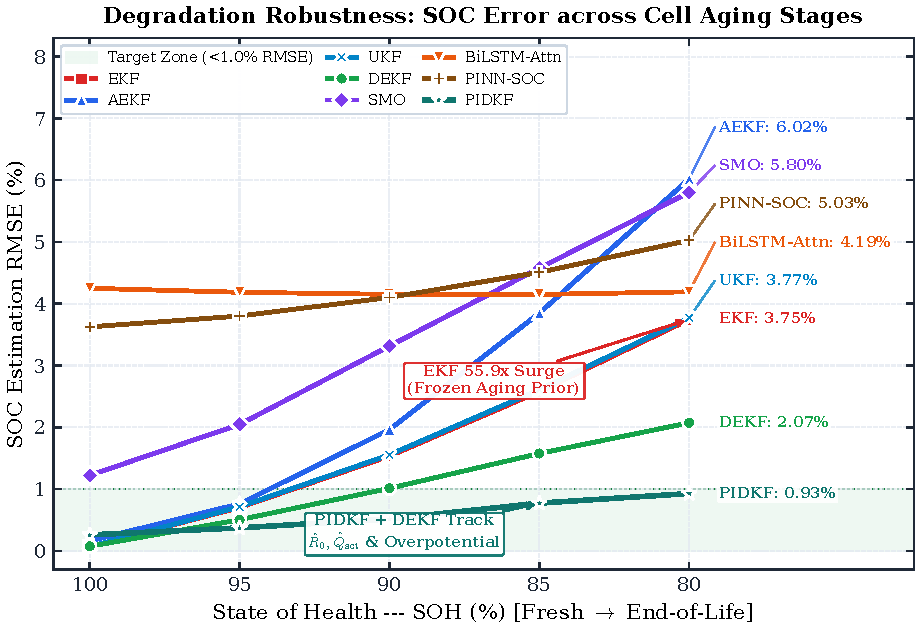
\includegraphics[width=0.88\linewidth]{fig4.pdf}
\caption{Evolution of SOC estimation RMSE as battery SOH degrades from $100\%$ down to $80\%$ on unseen UDDS, illustrating the $55.9$-fold degradation of standard EKF versus DEKF ($2.073\%$) and sub-percent PIDKF ($0.928\pm0.027\%$).\label{fig:aging}}
\end{figure}

\subsection[Phase 3: Thermal Robustness Across Wide Environmental Regimes (0 to 45 deg C)]{Phase 3: Thermal Robustness Across Wide Environmental Regimes ($0^\circ\text{C}$ to $45^\circ\text{C}$)}
Figure~\ref{fig:thermal} and Table~\ref{tab:3_thermal} compare tracking fidelity across $0^\circ\text{C}$, $25^\circ\text{C}$, and $45^\circ\text{C}$ on unseen UDDS under strictly fresh $25^\circ\text{C}$ nominal priors.

At $0^\circ\text{C}$, sluggish $\text{Li}^+$ desolvation (slower solvent shedding before interfacial insertion) expands ohmic and charge-transfer resistance nearly threefold via Arrhenius kinetics (Eqs.~\eqref{eqn:arrh_r0}--\eqref{eqn:arrh_ri}, Table~\ref{tab:ecm_params}), pushing fixed-prior EKF, UKF, and SMO to $9.566\%\text{--}10.258\%$ RMSE (Table~\ref{tab:3_thermal}, Fig.~\ref{fig:thermal}). While DEKF cuts $0^\circ\text{C}$ error down to $3.806\%$ by adapting $\hat{R}_{0,k}$, holding $R_1$ and $R_2$ at room-temperature values leaves substantial unmodeled polarization lag and capacity mismatch across high-rate transients. Similarly, standalone neural baselines exhibit high seed-to-seed variance at $0^\circ\text{C}$ ($\pm 1.670\text{--}5.435\%$) and large warm-temperature drift ($4.489\text{--}6.853\%$ at $45^\circ\text{C}$). By absorbing thermal polarization residuals through its temperature-conditioned Butler--Volmer compensator, the proposed \textbf{PIDKF} achieves the lowest tracking error at both thermal extremes ($2.526\pm0.098\%$ at $0^\circ\text{C}$ and $0.573\pm0.019\%$ at $45^\circ\text{C}$), consistent with the real-world NASA PCoE $4^\circ\text{C}/43^\circ\text{C}$ trends in Table~\ref{tab:10_tier1}.

\begin{table}[htbp]
\caption{Thermal robustness comparison across ambient temperatures on unseen UDDS [Tier~2 Calibrated Co-Simulation] (RMSE in \%; $5$-seed Mean$\pm$SD at $0^\circ\text{C}$ and $45^\circ\text{C}$ for neural models).\label{tab:3_thermal}}
\centering{%
\small\renewcommand{\arraystretch}{1.25}%
\begin{tabular*}{\linewidth}{@{\extracolsep{\fill}}lccc}
\toprule
Algorithm & 0$^\circ$C & 25$^\circ$C & 45$^\circ$C \\
\midrule
EKF & 9.566 & \textbf{0.067} & 1.467 \\
AEKF & 8.455 & 0.161 & 1.623 \\
UKF & 9.673 & 0.069 & 1.454 \\
DEKF & 3.806 & 0.073 & 1.034 \\
SMO & 10.258 & 1.222 & 3.402 \\
BiLSTM-Attn & $7.360\pm5.435$ & 4.250 & $6.158\pm1.227$ \\
PINN-SOC & $8.402\pm4.749$ & 3.625 & $6.853\pm2.281$ \\
MLP (Unconstrained) & $5.972\pm1.670$ & 3.201 & $4.489\pm0.982$ \\
\textbf{PIDKF (Proposed)} & \textbf{2.526$\pm$0.098} & 0.258 & \textbf{0.573$\pm$0.019} \\
\bottomrule
\end{tabular*}
}%
\end{table}

\begin{figure}[htbp]
\centering
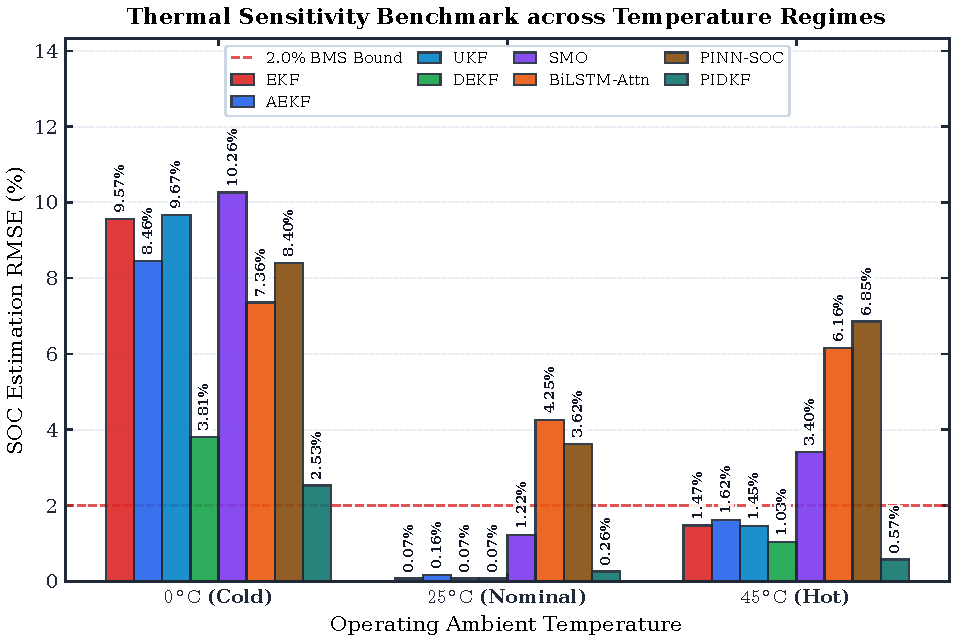
\includegraphics[width=0.88\linewidth]{fig5.pdf}
\caption{Algorithmic thermal sensitivity under cold ($0^\circ\text{C}$), nominal ($25^\circ\text{C}$), and elevated ($45^\circ\text{C}$) ambient temperatures.\label{fig:thermal}}
\end{figure}

\subsection[Phase 4: Convergence Under Large Initial State Uncertainty]{Phase 4: Convergence Under Large Initial State Uncertainty ($\Delta\text{SOC}_0 = -40\%$)}
In real-world BMS operation, initialization errors arise from prolonged parking, self-discharge, or battery replacement. Figure~\ref{fig:conv} and Table~\ref{tab:4_conv} evaluate convergence trajectories following an abrupt $\Delta\text{SOC}_0 = -40\%$ initialization shock ($\text{SOC}_0^{\text{true}} = 0.85$ and initial estimate $\hat{z}_0 = 0.45$ at step $k=0$).

Under this large initial offset, fixed-prior UKF and EKF enter the $\le 5\%$ operational corridor fastest ($7.0\text{--}8.0\text{ s}$) and attain the tightest post-reach tracking ($1.98\text{--}2.02\%$ $\text{MaxE}_{\text{dyn}}$), while SMO settles cleanly within $10\text{--}11\text{ s}$ at the expense of a sharp initial $36.95\%$ transient excursion (Table~\ref{tab:4_conv}, Fig.~\ref{fig:conv}). Dual state--parameter filters (DEKF and PIDKF) exhibit longer initial settling ($t_{\text{settle}}^{(5\%)} = 288.0\text{ s}$ and $336.0\text{ s}$; $t_{\text{reach}}^{(2\%)} = 966.0\text{ s}$ and $1089.2\text{ s}$) because the large early voltage residual transiently perturbs $\hat{R}_{0,k}$ before parameter covariance contracts, after which both track smoothly ($\text{MaxE}_{\text{dyn}} = 2.03\text{--}2.05\%$). By contrast, BiLSTM-Attn fails to converge into the $2\%$ or $5\%$ tolerances ($39.99\%$ peak, $7.470\%$ RMSE), and memoryless feedforward PINN-SOC and Unconstrained MLP only reach the $2\%$ threshold coincidentally mid-discharge before drifting back outside during subsequent load pulses ($t_{\text{settle}}^{(5\%)} = 1601.6\text{--}1747.0\text{ s}$).

\begin{table}[htbp]
\caption{Convergence metrics under initial state uncertainty on unseen UDDS [Tier~2 Calibrated Co-Simulation, $25^\circ\text{C}$, $100\%$ SOH] ($\Delta\text{SOC}_0 = -40\%$ initial error; $5$-seed mean for neural models).\label{tab:4_conv}}
\centering{%
\small\renewcommand{\arraystretch}{1.25}
\begin{tabular*}{\linewidth}{@{\extracolsep{\fill}}lccccc}
\toprule
Algorithm & $t_{\text{reach}}^{(2\%)}$ (s) & $t_{\text{settle}}^{(5\%)}$ (s) & RMSE (\%) & MaxE (\%) & $\text{MaxE}_{\text{dyn}}^\dagger$ (\%) \\
\midrule
EKF & 510.0 & 8.0 & 1.876 & 10.29 & \textbf{1.98} \\
AEKF & 805.0 & 119.0 & 2.734 & \textbf{6.49} & 2.07 \\
UKF & 463.0 & \textbf{7.0} & \textbf{1.817} & 11.14 & 2.02 \\
DEKF & 966.0 & 288.0 & 3.437 & 10.29 & 2.03 \\
SMO & \textbf{11.0} & 10.0 & 2.248 & 36.95 & 4.26 \\
BiLSTM-Attn & N/A$^\S$ & N/A$^\S$ & 7.470 & 39.99 & 20.23 \\
PINN-SOC & 522.2 & 1747.0$^*$ & 4.492 & 8.74 & 8.08 \\
MLP (Unconstrained) & 224.6 & 1601.6$^*$ & 4.008 & 8.68 & 8.18 \\
PIDKF (Proposed) & 1089.2 & 336.0 & 3.653 & 10.51 & 2.05 \\
\bottomrule
\end{tabular*}
\vspace{2pt}
{\raggedright\scriptsize $^\dagger\text{MaxE}_{\text{dyn}}$: peak dynamic error after first entry into $2\%$ ($t > t_{\text{reach}}^{(2\%)}$). $^\S$Fails to reach $\le 2\%$ or settle within $\le 5\%$ across the cycle. $^*$Memoryless feedforward inference lacks recursive settling and exits $\le 5\%$ repeatedly after early trajectory crossings.\par}
}%
\end{table}

\begin{figure}[htbp]
\centering
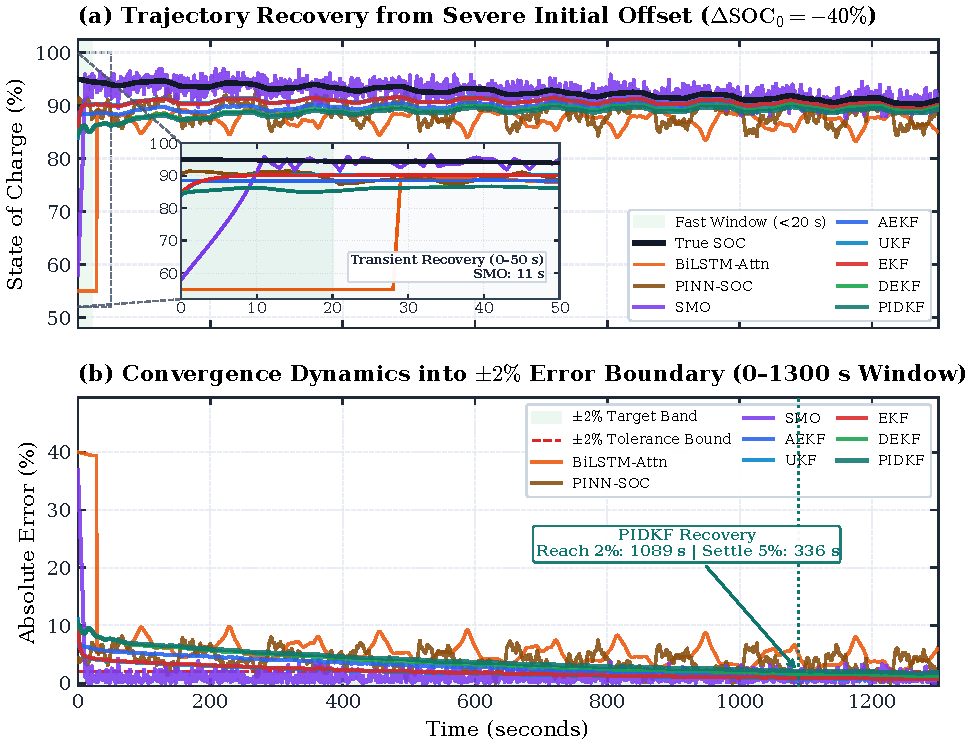
\includegraphics[width=0.88\linewidth]{fig6.pdf}
\caption{Transient convergence trajectories and $2\%$ tolerance recovery following a $-40\%$ initial SOC estimation shock on unseen UDDS ($25^\circ\text{C}$, $100\%$ SOH).\label{fig:conv}}
\end{figure}

\subsection{Phase 5: Multi-Attribute Radar Trade-Off and Pareto Analysis}
Figure~\ref{fig:radar} synthesizes algorithmic trade-offs across five normalized dimensions scored on a $1\text{--}10$ scale: Nominal Accuracy, Aging Robustness, Thermal Robustness, Convergence Speed, and Computational (Embedded) Efficiency. Classical EKF leads nominal accuracy ($9.75/10$), fast settling ($9.27/10$), and embedded simplicity ($9.08/10$) yet drops sharply under aging ($4.01/10$) and thermal stress ($3.10/10$). DEKF raises aging and thermal scores substantially ([$9.67$, $6.68$, $6.97$, $7.98$, $8.31$]), while the proposed \textbf{PIDKF} delivers the most balanced multi-attribute envelope across all five criteria ([$8.57$, $8.52$, $8.06$, $7.76$, $7.88$]), confirming that coupling dual parameter adaptation with a lightweight constrained compensator bridges real-world robustness gaps without sacrificing microcontroller efficiency.

\begin{figure}[htbp]
\centering
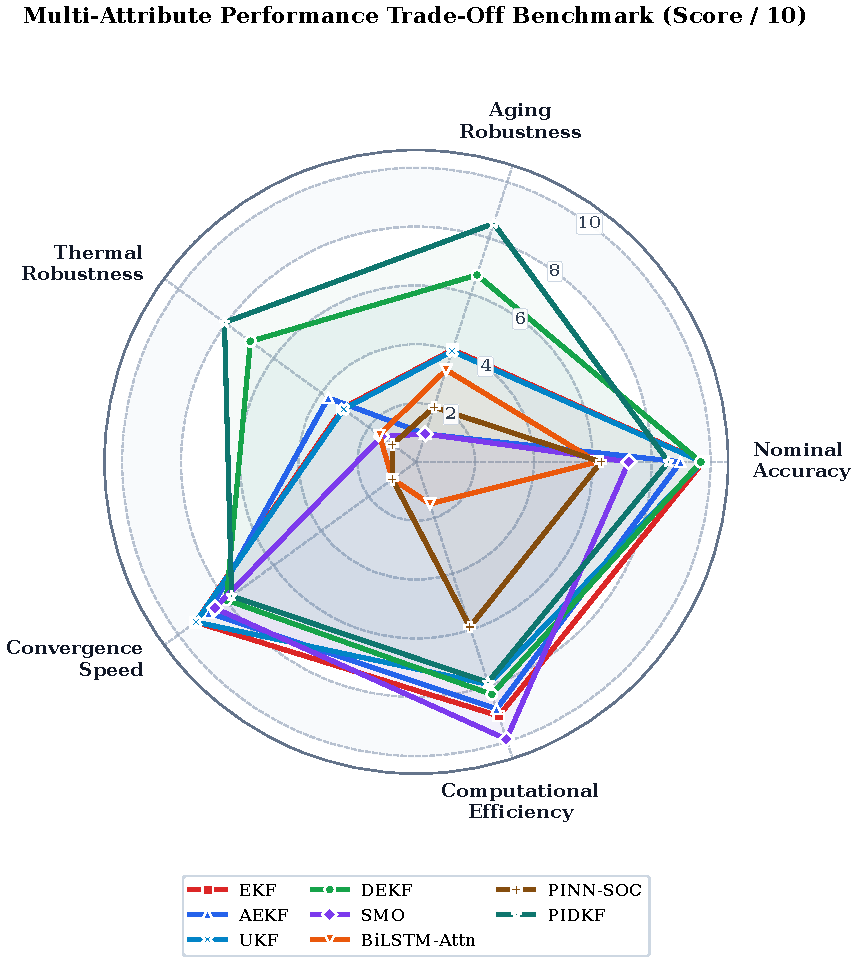
\includegraphics[width=0.72\linewidth]{fig7.pdf}
\caption{Multi-attribute radar comparison across 5 engineering dimensions illustrating algorithmic trade-offs.\label{fig:radar}}
\end{figure}

\subsection[Phase 6: Multi-Chemistry Generalization: LiFePO4 (LFP) Flat Plateau]{Phase 6: Multi-Chemistry Generalization: $\text{LiFePO}_4$ (LFP) Flat Plateau}
Figure~\ref{fig:lfp} and Table~\ref{tab:5_lfp} evaluate cross-chemistry generalization on identical unseen $25^\circ\text{C}$ UDDS (and FUDS) schedules across sloping-OCV NMC and flat-plateau $\text{LiFePO}_4$ ($100\%$ SOH) using chemistry-matched nominal priors and active 4-state hysteresis compensation.

Incorporating dynamic hysteresis transforms the LFP tracking landscape (Table~\ref{tab:5_lfp}, Fig.~\ref{fig:lfp}). Removing the hysteresis state causes the No-Hysteresis EKF control to stall at $0.401\%$ RMSE ($0.698\%$ MaxE) due to $\pm 30\;\mathrm{mV}$ charge--discharge voltage offset; enabling 4-state hysteresis cancels that systematic bias and lowers EKF and DEKF errors nearly eightfold to $0.049\text{--}0.051\%$ on UDDS ($0.050\text{--}0.055\%$ on FUDS), while PIDKF tracks seamlessly across both chemistries ($0.134\pm0.040\%$ LFP UDDS, $0.143\%$ LFP FUDS; $0.258\pm0.111\%$ NMC UDDS). Meanwhile, purely data-driven networks retrained cleanly on LFP DST still incur $1.538\text{--}4.492\%$ RMSE on unseen LFP UDDS and FUDS schedules.

\begin{table}[htbp]
\caption{Cross-chemistry benchmark comparing NMC and $\text{LiFePO}_4$ on identical unseen schedules [Tier~2 Calibrated Co-Simulation, $25^\circ\text{C}$, $100\%$ SOH, 4-state hysteresis active on LFP].\label{tab:5_lfp}}
\centering{%
\small\renewcommand{\arraystretch}{1.22}
\setlength{\tabcolsep}{2.2pt}
\begin{tabular*}{\linewidth}{@{\extracolsep{\fill}}lcccc}
\toprule
Algorithm & NMC UDDS (\%) & LFP UDDS (\%) & LFP MaxE (\%) & LFP FUDS (\%) \\
\midrule
EKF & \textbf{0.067} & \textbf{0.049} & 0.297 & 0.055 \\
EKF (No Hyst.\ Control) & -- & 0.401 & 0.698 & -- \\
AEKF & 0.161 & 0.388 & 0.786 & 0.682 \\
UKF & 0.069 & 0.241 & 3.309 & 0.281 \\
DEKF & 0.073 & 0.051 & \textbf{0.288} & \textbf{0.050} \\
SMO & 1.222 & 0.470 & 2.084 & 0.590 \\
BiLSTM-Attn & $4.250\pm0.653$ & $1.538\pm0.212$ & 3.541 & 1.758 \\
PINN-SOC & $3.625\pm0.851$ & $4.492\pm0.517$ & 7.557 & 3.573 \\
PIDKF (Proposed) & $0.258\pm0.111$ & $0.134\pm0.040$ & 0.334 & 0.143 \\
\bottomrule
\end{tabular*}
}%
\end{table}

\begin{figure}[htbp]
\centering
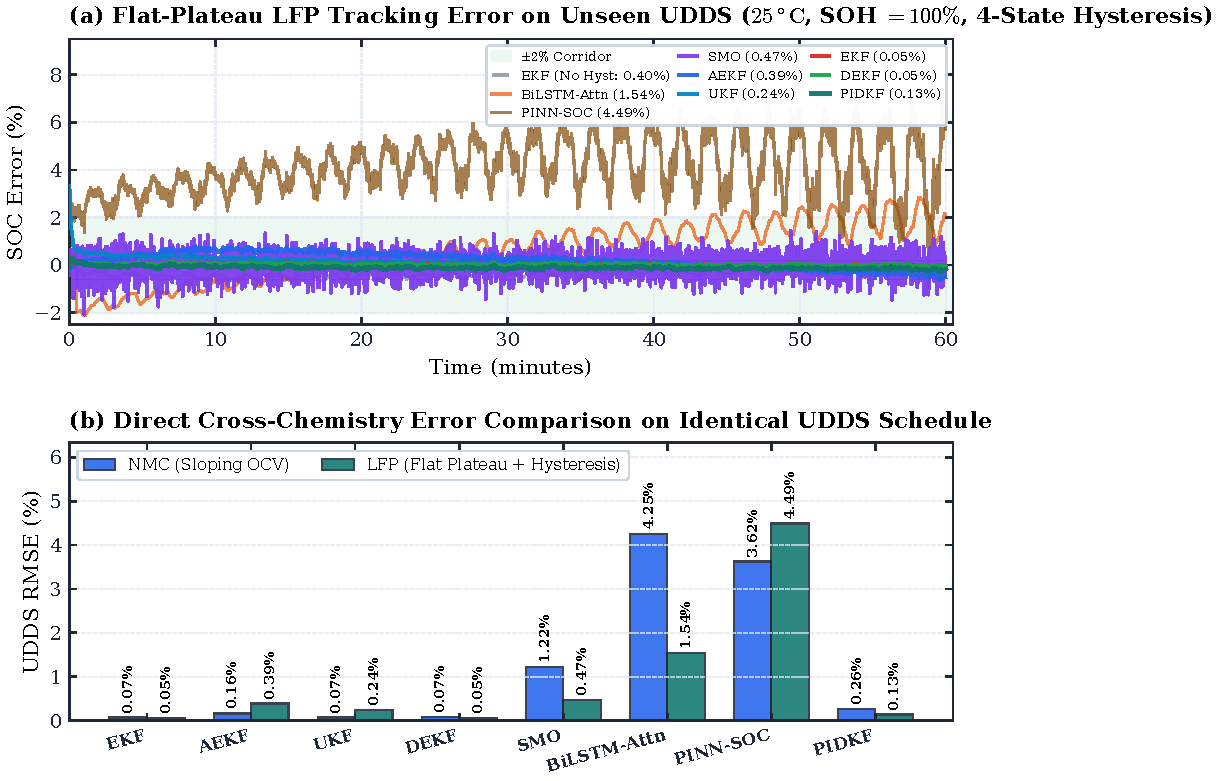
\includegraphics[width=0.88\linewidth]{fig8.pdf}
\caption{Cross-chemistry comparison and estimation error along the flat $\text{LiFePO}_4$ voltage plateau ($25^\circ\text{C}$, unseen UDDS, 4-state hysteresis active vs.\ uncompensated control).\label{fig:lfp}}
\end{figure}

\subsection{Phase 7: Sensor Corruption and Environmental Stress Testing}
Table~\ref{tab:6_sensor} and Fig.~\ref{fig:sensor} document 2-hour UDDS resilience under simultaneous $+0.25\text{ A}$ Hall current-sensor bias drift and $25\text{ mV}$ RMS switching EMI ripple.

Without voltage innovation feedback, open-loop Coulomb counting integrates the $+0.25\text{ A}$ direct-current (DC) bias linearly into $14.394\%$ RMSE and $24.840\%$ final-60s end-of-cycle drift (Table~\ref{tab:6_sensor}, Fig.~\ref{fig:sensor}). Closed-loop observers reject unbounded runaway: \textbf{PIDKF achieves the lowest overall RMSE ($1.308\pm0.099\%$) and tightest final-60s residual drift ($1.237\%$)}, closely followed by EKF ($1.475\%$) and DEKF ($1.579\%$), because inflated measurement variance $R_{\text{eff},k}$ prevents high-frequency $25\;\mathrm{mV}$ EMI from entering the gain while closed-loop OCV feedback bounds current-offset drift. Conversely, aggressive SMO switching amplifies the $25\;\mathrm{mV}$ EMI noise into $4.354\%$ RMSE ($14.116\%$ MaxE) with $2.709\%$ final-60s residual drift.

\begin{table}[htbp]
\caption{Robustness under $+0.25\text{ A}$ Hall current bias and $25\text{ mV}$ EMI over 2-hour UDDS [Tier~2 Calibrated Co-Simulation].\label{tab:6_sensor}}
\centering{%
\small\renewcommand{\arraystretch}{1.22}
\begin{tabular*}{\linewidth}{@{\extracolsep{\fill}}lccc}
\toprule
Algorithm & RMSE (\%) & MaxE (\%) & Final-60s Drift (\%) \\
\midrule
Coulomb Counting & 14.394 & 24.943 & 24.840 \\
EKF & 1.475 & \textbf{2.970} & 1.406 \\
AEKF & 1.719 & 3.310 & 1.605 \\
DEKF & 1.579 & 3.235 & 1.584 \\
SMO & 4.354 & 14.116 & 2.709 \\
\textbf{PIDKF (Proposed)} & $\mathbf{1.308 \pm 0.099}$ & 3.197 & \textbf{1.237} \\
\bottomrule
\end{tabular*}
}%
\end{table}

\begin{figure}[htbp]
\centering
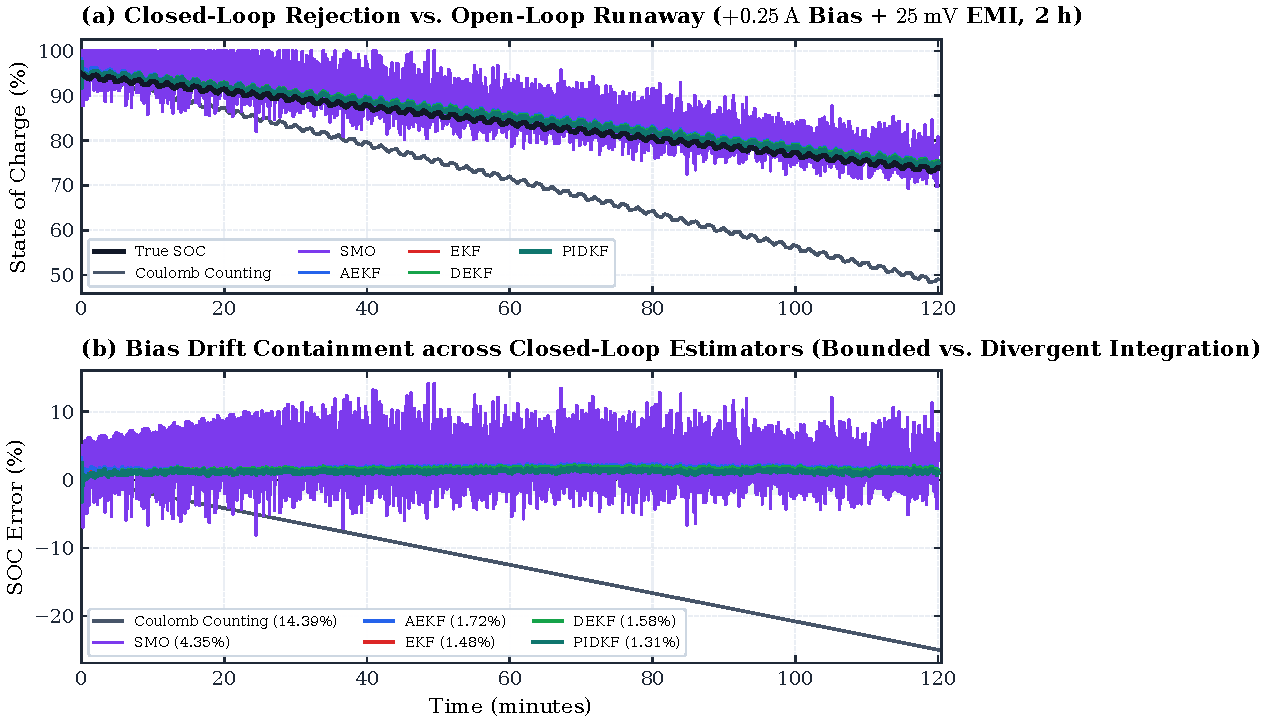
\includegraphics[width=0.88\linewidth]{fig9.pdf}
\caption{Observer robustness under current sensor bias drift ($+0.25\text{ A}$) and $25\text{ mV}$ EMI ripple across a 2-hour UDDS run.\label{fig:sensor}}
\end{figure}

\subsection{Phase 8: Real Experimental Electrochemical Impedance Spectroscopy (EIS) Analysis}
Figure~\ref{fig:eis} fits the Randles--CPE circuit with series test-lead/tab inductance $L$ directly to real 39-frequency ($0.1\;\mathrm{Hz}\text{--}5\;\mathrm{kHz}$) impedance spectra measured on NASA Ames PCoE cell \texttt{B0006} across Fresh, Mid-Life, and End-of-Test aging stages:
\begin{equation}\label{eqn:eis_randles}
Z(j\omega) = j\omega L + R_0 + \frac{R_{\text{ct}} + Z_w(j\omega)}{1 + (j\omega)^\alpha Q_{\text{cpe}} \left(R_{\text{ct}} + Z_w(j\omega)\right)}, \qquad Z_w(j\omega) = \sigma_w \omega^{-1/2}(1 - j),
\end{equation}
where $Z(j\omega)$ is the complex electrochemical impedance at angular frequency $\omega$ ($\mathrm{rad}\cdot\mathrm{s}^{-1}$), $Z_w(j\omega)$ is the semi-infinite Warburg diffusion impedance, $R_0 = R_{\text{ohm}} + R_{\text{sei}}$ is bulk ohmic resistance, $R_{\text{ct}}$ is charge-transfer resistance, $Q_{\text{cpe}}$ is the constant-phase element ($\mathrm{mF}\cdot\mathrm{s}^{\alpha-1}$) with depression exponent $\alpha$, and $\sigma_w$ is the Warburg coefficient ($\mathrm{m\Omega}\cdot\mathrm{s}^{-1/2}$). Nonlinear complex least-squares fitting achieves $<2.8\%$ relative RMS error at every checkpoint:
\begin{itemize}
\item \textbf{Fresh ($\sim 100\%$ SOH):} $R_0 = 56.67 \pm 2.01\;\mathrm{m}\Omega$, $R_{\text{ct}} = 22.37 \pm 2.77\;\mathrm{m}\Omega$, $L = 0.203\;\upmu\mathrm{H}$, $Q_{\text{cpe}} = 1633.5\;\mathrm{mF}\cdot\mathrm{s}^{\alpha-1}$ ($\alpha = 0.482 \pm 0.068$), $\sigma_w = 0.29\;\mathrm{m}\Omega\cdot\mathrm{s}^{-1/2}$ (RMS $1.82\;\mathrm{m}\Omega$, $2.54\%$).
\item \textbf{Mid-Life ($\sim 90\%$ SOH):} $R_0 = 65.62 \pm 2.30\;\mathrm{m}\Omega$, $R_{\text{ct}} = 27.19 \pm 3.43\;\mathrm{m}\Omega$, $L = 0.217\;\upmu\mathrm{H}$, $Q_{\text{cpe}} = 1936.3\;\mathrm{mF}\cdot\mathrm{s}^{\alpha-1}$ ($\alpha = 0.454 \pm 0.067$), $\sigma_w = 0.31\;\mathrm{m}\Omega\cdot\mathrm{s}^{-1/2}$ (RMS $2.10\;\mathrm{m}\Omega$, $2.54\%$).
\item \textbf{End-of-Test ($\sim 75\%$ SOH):} $R_0 = 64.14 \pm 4.87\;\mathrm{m}\Omega$, $R_{\text{ct}} = 38.89 \pm 8.04\;\mathrm{m}\Omega$, $L = 0.253\;\upmu\mathrm{H}$, $Q_{\text{cpe}} = 3037.6\;\mathrm{mF}\cdot\mathrm{s}^{\alpha-1}$ ($\alpha = 0.344 \pm 0.079$), $\sigma_w \approx 0.00\;\mathrm{m}\Omega\cdot\mathrm{s}^{-1/2}$ (RMS $2.40\;\mathrm{m}\Omega$, $2.75\%$).
\end{itemize}
These experimental spectra confirm a key physical asymmetry encoded in our Tier~2 aging model: while high-frequency $R_0$ stabilizes or grows modestly ($+13.2\%$), real interfacial charge-transfer resistance $R_{\text{ct}}$ widens by $+73.8\%$ alongside severe CPE depression ($\alpha: 0.482 \rightarrow 0.344$, reflecting growing porous-electrode heterogeneity). Physically, high-frequency alternating-current (AC) $R_0$ ($\sim 44\text{--}57\;\mathrm{m}\Omega$) differs from millisecond-scale DC pulse $R_0$ because double-layer capacitance shunts $R_{\text{ct}}$ at kilohertz frequencies whereas $1\;\mathrm{s}$ BMS sampling captures fast SEI/charge-transfer polarization coupled into dynamic $U_1$ and $\hat{R}_0$.

\begin{figure}[htbp]
\centering
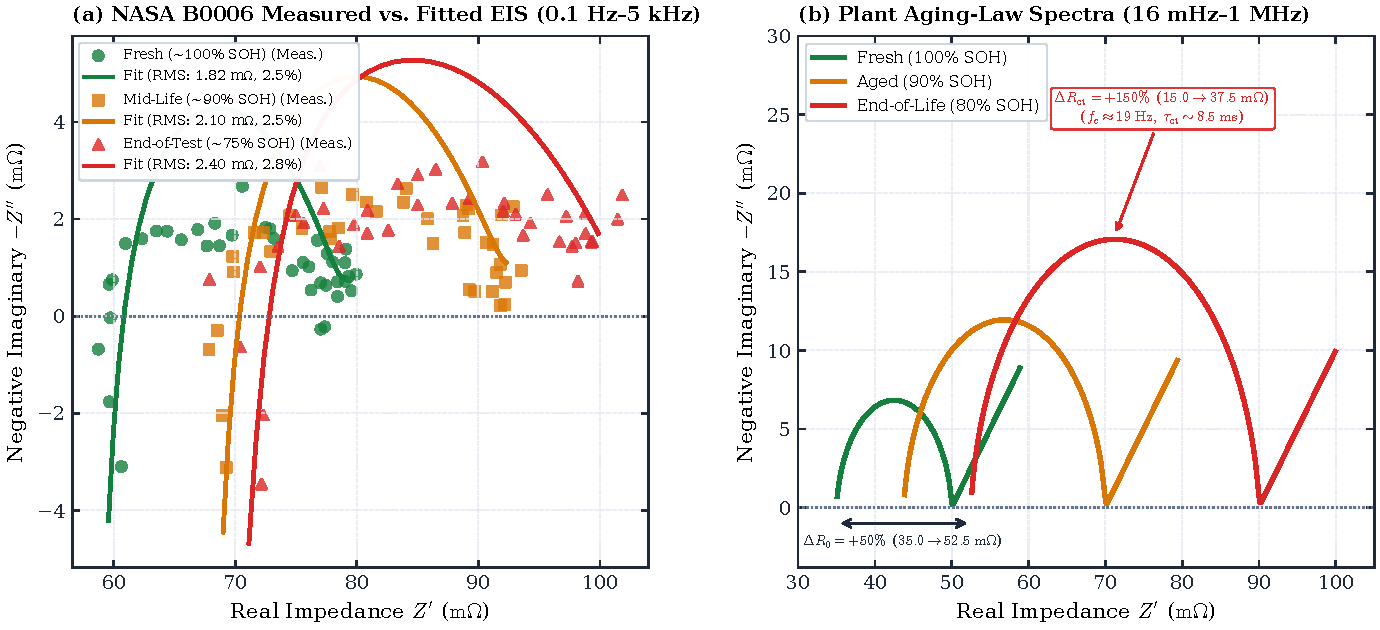
\includegraphics[width=0.88\linewidth]{fig10.pdf}
\caption{Tier~1 real NASA PCoE \texttt{B0006} Nyquist impedance spectra ($0.1\;\mathrm{Hz}\text{--}5\;\mathrm{kHz}$, 39 frequencies) and fitted Randles--CPE+L curves across Fresh, Mid-Life, and End-of-Test aging stages.\label{fig:eis}}
\end{figure}

\subsection{Phase 9: Module and Pack-Level Scaling (8S Series Pack)}
Table~\ref{tab:7_pack} and Fig.~\ref{fig:pack} evaluate scalability to an 8S series battery pack subjected to cell-to-cell capacity and resistance relative standard deviations ($\sigma_Q = 3.0\%$, $\sigma_R = 10.0\%$)~\cite{Yang2024degradation,Zheng2018inconsistency} and coupled thermal-SEI aging. Because interior cell~\#4 sits between neighbors with weaker cooling than perimeter cells, UDDS cycling elevates its core temperature by $+2.63^\circ\text{C}$, accelerating SEI degradation to $Q_{\text{act}} = 1.703\;\mathrm{Ah}$ ($85.0\%$ SOH, $R_0 = 60.5\;\mathrm{m}\Omega$). Under continuous load, cell~\#4 reaches deep depletion ($8.78\%$ SOC) while the string mean remains higher.

A lumped observer driven solely by total pack string voltage $V_{\text{string}}$ incurs $2.480\%$ mean-pack RMSE ($3.981\%$ MaxE) and overestimates weakest cell~\#4 by up to $+3.303\%$ peak ($1.317\%$ RMSE), masking incipient over-discharge below the anode potential window where copper current-collector dissolution risk emerges (Table~\ref{tab:7_pack}, Fig.~\ref{fig:pack}). Even distributed per-cell DEKF leaves $2.157\%$ weakest-cell RMSE ($4.369\%$ MaxE) because frozen $R_1, R_2$ lags during hot interior transients. In contrast, \textbf{Distributed PIDKF} confines mean-pack error to $0.223\%$ RMSE and slashes weakest-cell~\#4 RMSE to $0.544\%$, protecting series packs against localized over-discharge without extra impedance hardware.

\begin{table}[htbp]
\caption{Series 8S pack benchmark with cell-to-cell thermal-SEI inconsistency [Tier~2 Co-Simulation].\label{tab:7_pack}}
\centering{%
\small\renewcommand{\arraystretch}{1.22}
\setlength{\tabcolsep}{2.0pt}
\begin{tabular*}{\linewidth}{@{\extracolsep{\fill}}lcccc}
\toprule
Architecture & Target State & RMSE (\%) & MaxE (\%) & Safety Margin Risk \\
\midrule
Lumped Pack Observer & Mean Pack SOC & 2.480 & 3.981 & Moderate \\
\textbf{Distributed PIDKF} & \textbf{Mean Pack SOC} & \textbf{0.223} & \textbf{1.511} & \textbf{None (Bounded)} \\
Lumped Pack Observer & Weakest Cell \#4 & 1.317 & 3.303$^\dagger$ & High (Cu Dissolution) \\
Distributed DEKF & Weakest Cell \#4 & 2.157 & 4.369 & Transient $R_1/R_2$ Lag \\
\textbf{Distributed PIDKF} & \textbf{Weakest Cell \#4} & \textbf{0.544} & 4.228 & \textbf{Bounded Error} \\
\bottomrule
\end{tabular*}%
\vspace{2pt}
{\raggedright\scriptsize $^\dagger$Peak $+3.303\%$ optimistic overestimation on cell~\#4 near $8.78\%$ end-of-discharge SOC.\par}
}%
\end{table}

\begin{figure}[htbp]
\centering
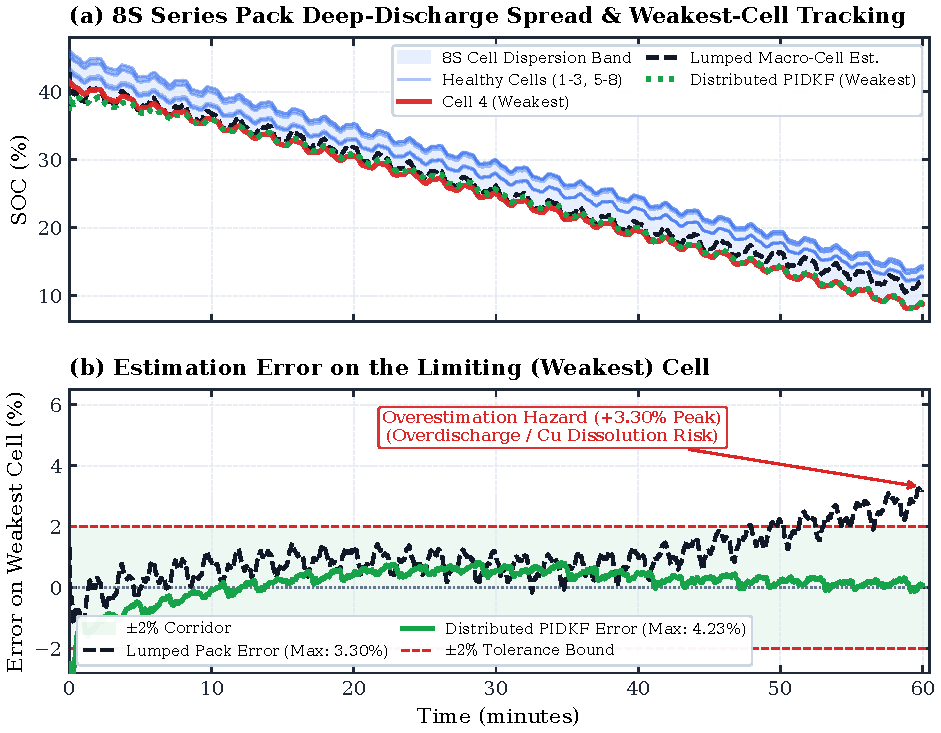
\includegraphics[width=0.88\linewidth]{fig11.pdf}
\caption{Series-connected 8S battery pack tracking comparing lumped pack deficiency against distributed DEKF and distributed PIDKF on weakest thermally stressed cell~\#4.\label{fig:pack}}
\end{figure}

\subsection{Phase 10: Analytical ARMv7E-M Sizing, PIDKF Ablation, and Tier 1 Cycler Validation}\label{sec:hw_profiling}
Finally, a practical BMS estimator must fit within automotive microcontroller budgets while maintaining fidelity on degraded cells and real laboratory cyclers. Rather than claiming unmeasured hardware timer dumps, static RAM and Flash footprints were audited directly from zero-heap ANSI-C99 reference kernels (\texttt{embedded\_c/}), and Cortex-M4F ($168\;\mathrm{MHz}$) and Cortex-M7 ($480\;\mathrm{MHz}$) instruction cycles and latencies were computed analytically via ARMv7E-M floating-point operation accounting (Table~\ref{tab:8_embedded}, Fig.~\ref{fig:embedded}). For PIDKF, exporting all $257$ trained \texttt{float32} MLP weights ($1,028\;\mathrm{B}$) to \texttt{embedded\_c/pidkf\_weights.h} confirmed bit-consistent single-step voltage compensation against PyTorch ($\max|\Delta\delta\hat{V}| = 2.64\times 10^{-5}\;\mathrm{V} < 10^{-4}\;\mathrm{V}$, where $\Delta\delta\hat{V}$ denotes the C99-to-PyTorch compensator difference).

\begin{table}[htbp]
\caption{Static ANSI-C99 memory sizing and analytical ARMv7E-M execution audit across $168\;\mathrm{MHz}$ Cortex-M4F and $480\;\mathrm{MHz}$ Cortex-M7 MCUs (zero dynamic allocation).\label{tab:8_embedded}}
\centering{%
\small\renewcommand{\arraystretch}{1.22}
\setlength{\tabcolsep}{3pt}
\resizebox{\linewidth}{!}{%
\begin{tabular}{lccccccc}
\toprule
Algorithm & Params & FLOPs/Step & M4F Cycles (Est.) & RAM (B) & Flash (B) & Est.\ M4F ($\upmu\mathrm{s}$) & Est.\ M7 ($\upmu\mathrm{s}$) \\
\midrule
SMO & 0 & 165 & 260 & 104 & 1,850 & 1.55 & 0.37 \\
EKF & 0 & 410 & 620 & 220 & 3,120 & 3.69 & 0.89 \\
AEKF & 0 & 540 & 810 & 232 & 3,840 & 4.82 & 1.16 \\
DEKF & 0 & 960 & 1,410 & 324 & 5,280 & 8.39 & 2.03 \\
UKF & 0 & 1,420 & 2,180 & 524 & 6,150 & 12.98 & 3.13 \\
\textbf{PIDKF (Proposed)} & \textbf{257} & \textbf{1,540} & \textbf{2,980} & \textbf{364} & \textbf{7,428} & \textbf{17.74} & \textbf{4.28} \\
PINN-SOC & 6,690 & 13,500 & 23,600 & 796 & 29,160 & 140.48 & 33.91 \\
BiLSTM-Attn & 13,698 & 1,680,000 & 2,850,000 & 8,160 & 58,992 & 16,964.29 & 4,094.83 \\
\bottomrule
\end{tabular}%
}%
}%
\vspace{2pt}
{\raggedright\scriptsize Note: RAM (B) sums persistent filter state \texttt{struct}s and local stack scratch; Flash (B) sums exported \texttt{float32} weights ($4\;\mathrm{B}$/param) and compiled Thumb-2 kernel size estimates. Under a $16$-cell pack at $10\;\mathrm{Hz}$ ($100\;\mathrm{ms}$ task period), PIDKF occupies $0.28\%$ Cortex-M4F CPU load versus $271.4\%$ (infeasible) for BiLSTM-Attn.\par}
\end{table}

\begin{figure}[htbp]
\centering
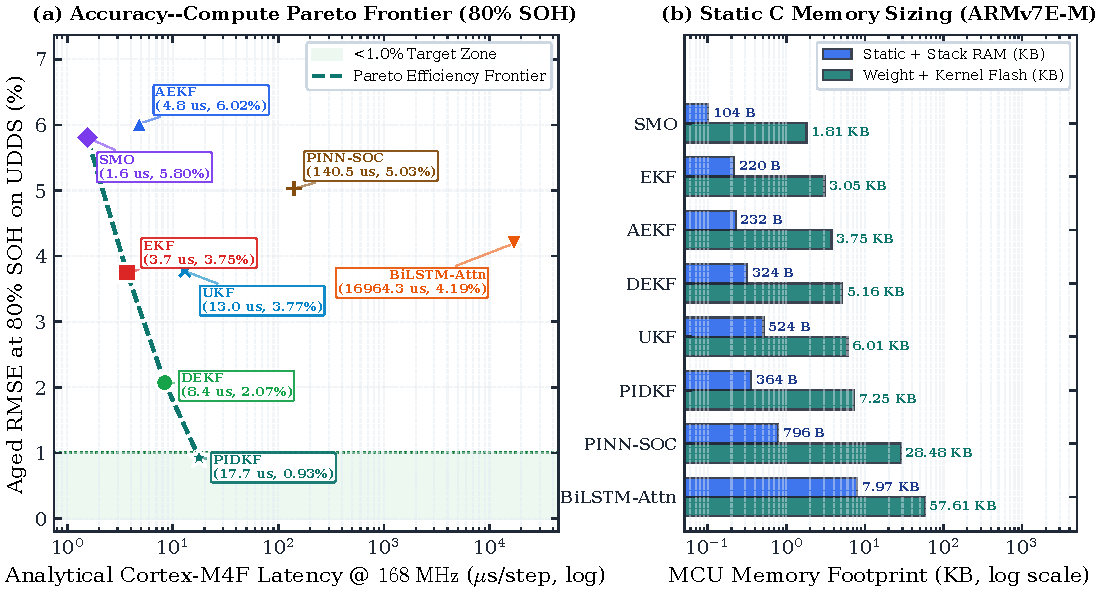
\includegraphics[width=0.92\linewidth]{fig12.pdf}
\caption{Embedded resource trade-off: (a)~Pareto accuracy--compute frontier on degraded $80\%$ SOH UDDS versus analytical $168\;\mathrm{MHz}$ Cortex-M4F latency, and (b)~static ANSI-C99 RAM and Flash memory footprint.\label{fig:embedded}}
\end{figure}

As shown in Table~\ref{tab:8_embedded} and Fig.~\ref{fig:embedded}, classical observers execute within $1.55\text{--}12.98\;\upmu\mathrm{s}$ per step with $<6.1\;\mathrm{KB}$ Flash. Conversely, BiLSTM-Attn incurs $1.68\;\text{million FLOPs (MFLOPs)}$ per $W=30$ sliding window ($16.96\;\mathrm{ms}$ on Cortex-M4F), exceeding real-time limits across a $16$-cell module at $10\;\mathrm{Hz}$. By decoupling neural backpropagation from the Kalman gain, \textbf{PIDKF} executes in an analytical budget of $17.74\;\upmu\mathrm{s}$ on Cortex-M4F ($4.28\;\upmu\mathrm{s}$ on Cortex-M7) using $364\;\mathrm{B}$ RAM and $7,428\;\mathrm{B}$ ($7.25\;\mathrm{KB}$) Flash ($0.28\%$ CPU utilization across $16$ cells at $10\;\mathrm{Hz}$), sitting cleanly at the Pareto accuracy--compute knee.

\begin{table}[htbp]
\caption{Tier~2 five-seed PIDKF ablation on unseen degraded UDDS ($85\%$ SOH, $25^\circ\text{C}$ and $0^\circ\text{C}$; Mean$\pm$SD over seeds $42\text{--}46$).\label{tab:9_pidkf}}
\centering{%
\small\renewcommand{\arraystretch}{1.22}
\setlength{\tabcolsep}{2.2pt}
\resizebox{\linewidth}{!}{%
\begin{tabular}{lccccc}
\toprule
& \multicolumn{2}{c}{NMC ($85\%$ SOH, $25^\circ\text{C}$)} & \multicolumn{2}{c}{LFP ($85\%$ SOH, $25^\circ\text{C}$)} & NMC ($85\%$, $0^\circ\text{C}$) \\
\cmidrule(lr){2-3} \cmidrule(lr){4-5} \cmidrule(lr){6-6}
Variant Configuration & RMSE (\%) & MaxE (\%) & RMSE (\%) & MaxE (\%) & RMSE (\%) \\
\midrule
Standard EKF & 2.207 & 4.763 & 1.495 & 3.794 & 15.886 \\
Baseline DEKF (No Hyst.) & 1.321 & 3.530 & 0.748 & 1.483 & 7.147 \\
DEKF + Hysteresis & 1.321 & 3.530 & \textbf{0.346} & \textbf{1.167} & 7.147 \\
DEKF + Black-Box MLP & $0.924\pm0.069$ & 3.686 & $0.895\pm0.123$ & 2.001 & $5.585\pm0.258$ \\
DEKF + Phys-Reg MLP (No Clamp) & $0.699\pm0.170$ & 3.383 & $0.688\pm0.068$ & 1.630 & \textbf{4.565$\pm$0.244} \\
Full PIDKF (Exact Jac.) & $1.894\pm0.495$ & \textbf{3.291} & $1.033\pm0.468$ & 2.117 & $7.808\pm0.508$ \\
\textbf{Full PIDKF (Exog.\ Approx.)} & \textbf{0.554$\pm$0.018} & 3.304 & $0.593\pm0.048$ & 1.463 & $5.092\pm0.037$ \\
\bottomrule
\end{tabular}%
}%
}%
\vspace{2pt}
{\raggedright\scriptsize Note: All neural variants use $5$ random Batch~A training seeds ($42\text{--}46$) and zero oracle aging/thermal leakage; MaxE reports the $5$-seed mean peak error.\par}
\end{table}

\begin{figure}[htbp]
\centering
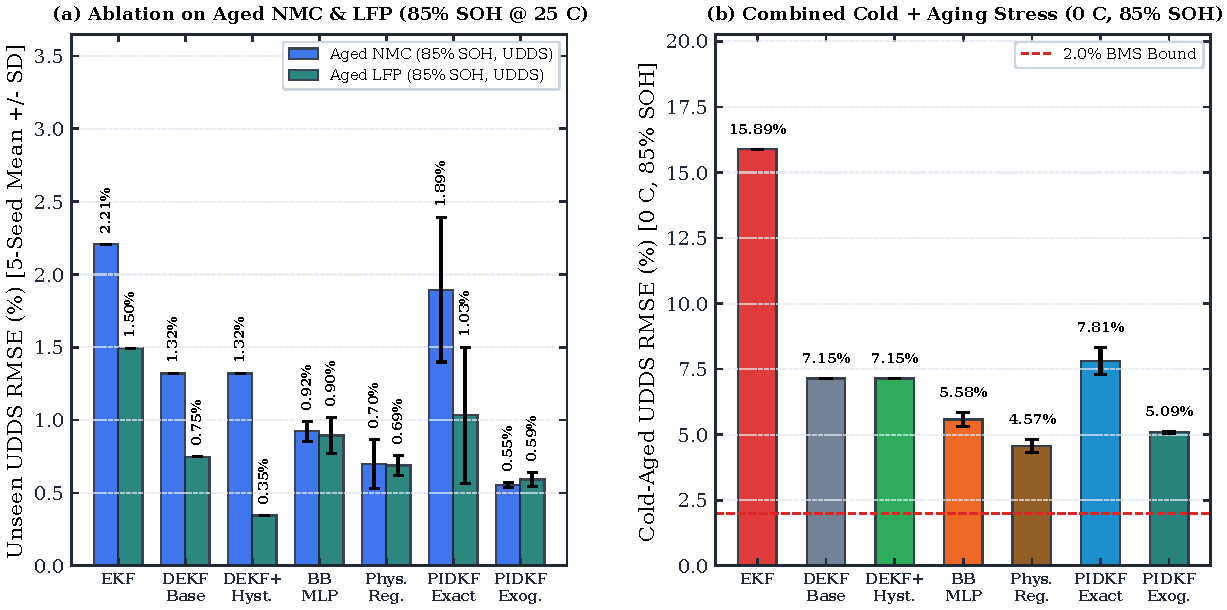
\includegraphics[width=0.92\linewidth]{fig13.pdf}
\caption{Five-seed PIDKF ablation on unseen degraded UDDS ($85\%$ SOH): (a)~sloped NMC vs.\ flat-plateau LFP at $25^\circ\text{C}$, and (b)~combined $0^\circ\text{C}$ cold plus $85\%$ aging stress.\label{fig:pidkf}}
\end{figure}

The five-seed Tier~2 ablation study (Table~\ref{tab:9_pidkf}, Fig.~\ref{fig:pidkf}) isolates three critical mechanisms. First, injecting exact automatic-differentiation neural Jacobians directly into $\mathbf{K}_k$ severely destabilizes convergence ($1.894\pm0.495\%$ NMC RMSE, $1.033\pm0.468\%$ LFP RMSE, $7.808\pm0.508\%$ cold NMC RMSE) because $\|\mathbf{J}_{\text{NN},k}\|_2 / \|\mathbf{H}_k\|_2$ averages $16.8\%$ (peak $28.7\%$) with non-smooth sign reversals across clamping and activation knees. \textbf{Exogenous sensitivity decoupling} shields $\mathbf{K}_k$, cutting aged NMC RMSE by $70.8\%$ to $0.554\pm0.018\%$ with tiny seed dispersion ($\pm 0.018\%$). Second, on sloped aged NMC at $25^\circ\text{C}$, hard Butler--Volmer passivity clamping lowers RMSE by $58.1\%$ over Baseline DEKF ($1.321\% \rightarrow 0.554\%$) and clearly outperforms both unconstrained black-box ($0.924\pm0.069\%$) and unclamped physics-regularized ($0.699\pm0.170\%$) neural MLPs. Third, our ablation exposes two deliberate physical trade-offs: on isothermal aged LFP, disabling the neural compensator (\texttt{DEKF + Hysteresis}) achieves the lowest LFP error ($0.346\%$ vs.\ $0.593\pm0.048\%$ for Full PIDKF) because weak plateau OCV slopes amplify any small neural bias, though Full PIDKF still outperforms hysteresis-free DEKF ($0.748\%$) and EKF ($1.495\%$). Likewise, under extreme combined $0^\circ\text{C}$ cold and $85\%$ aging stress where $R_1$ expands $7.1$-fold ($15.0\rightarrow 107.0\;\mathrm{m}\Omega$), true polarization peaks briefly exceed the $147\;\mathrm{mV}$ hard Butler--Volmer envelope; thus, \texttt{DEKF + Phys-Reg MLP (No Clamp)} reaches slightly lower mean RMSE ($4.565\pm0.244\%$ vs.\ $5.092\pm0.037\%$ for Full PIDKF), whereas Full PIDKF enforces formal ISS passivity and cuts cross-seed dispersion by $6.6$-fold ($\pm 0.244\% \rightarrow \pm 0.037\%$).

\begin{table}[htbp]
\caption{Tier~1 direct laboratory cycler validation on held-out XJTU Batch-5 (NMC532 Random Walk) and NASA Ames PCoE ($24^\circ\text{C}$ aging, $43^\circ\text{C}$ high-rate, and $4^\circ\text{C}$ cold discharge) datasets (RMSE in \%).\label{tab:10_tier1}}
\centering{%
\small\renewcommand{\arraystretch}{1.22}
\setlength{\tabcolsep}{2.2pt}
\resizebox{\linewidth}{!}{%
\begin{tabular}{lcccccccc}
\toprule
Test Cell & Cond. & SOH / $Q_{\text{act}}$ & EKF & AEKF & DEKF & SMO & BiLSTM / PINN$^\dagger$ & \textbf{PIDKF} \\
\midrule
\multicolumn{9}{l}{\emph{XJTU Batch-5 Held-Out Test Cells (Batch~B Dynamic Random Walk, Calibrated Strictly on Batch~A RW\_1/RW\_2)}} \\
\texttt{RW\_3} Fresh & $25^\circ\text{C}$ RW & $100.0\%$ & 1.796 & 1.889 & 1.490 & 5.025 & $2.175\pm0.135$ / $3.992\pm0.787$ & \textbf{1.425$\pm$0.058} \\
\texttt{RW\_4} Fresh & $25^\circ\text{C}$ RW & $100.0\%$ & 3.542 & 3.923 & \textbf{2.210} & 6.015 & $2.449\pm0.219$ / $4.742\pm0.891$ & $2.566\pm0.252$ \\
\texttt{RW\_3} Aged & $25^\circ\text{C}$ RW & $86.0\%$ & 2.241 & 2.259 & 2.397 & 5.851 & $5.994\pm0.246$ / $3.996\pm0.937$ & \textbf{2.034$\pm$0.132} \\
\texttt{RW\_4} Aged & $25^\circ\text{C}$ RW & $86.8\%$ & 2.983 & 3.041 & 3.044 & 6.622 & $5.854\pm0.233$ / $4.732\pm0.899$ & \textbf{2.750$\pm$0.138} \\
\midrule
\multicolumn{9}{l}{\emph{NASA Ames PCoE Cells (Calibrated on Fresh \texttt{B0005} Cyc.\ 0 @ $R_0 = 44.67\;\mathrm{m}\Omega$ from EIS)}} \\
\texttt{B0007} Fresh & $24^\circ\text{C}$ $2\text{ A}$ & $1.920\;\mathrm{Ah}$ & 0.799 & 0.799 & 0.787 & 0.890 & --$^\ddagger$ & \textbf{0.636$\pm$0.045} \\
\texttt{B0007} Aged & $24^\circ\text{C}$ $2\text{ A}$ & $1.553\;\mathrm{Ah}$ ($81\%$) & 3.900 & 3.965 & 2.246 & 6.185 & --$^\ddagger$ & \textbf{1.715$\pm$0.098} \\
\texttt{B0030} Hot & $43^\circ\text{C}$ $4\text{ A}$ & $1.757\;\mathrm{Ah}$ & 7.490 & 7.427 & \textbf{4.863} & 7.986 & --$^\ddagger$ & $4.940\pm0.131$ \\
\texttt{B0055} Cold & $4^\circ\text{C}$ $2\text{ A}$ & $1.253\;\mathrm{Ah}$ & 26.109 & 26.405 & 15.752 & 36.109 & --$^\ddagger$ & \textbf{9.562$\pm$0.122} \\
\texttt{B0056} Cold & $4^\circ\text{C}$ $2\text{ A}$ & $1.261\;\mathrm{Ah}$ & 30.218 & 30.696 & 19.545 & 39.633 & --$^\ddagger$ & \textbf{13.618$\pm$0.069} \\
\bottomrule
\end{tabular}%
}%
}%
\vspace{2pt}
{\raggedright\scriptsize $^\dagger$BiLSTM-Attn / PINN-SOC $5$-seed Mean$\pm$SD trained on Batch~A \texttt{RW\_1/RW\_2}; PIDKF MaxE on XJTU \texttt{RW\_3/4} spans $3.164\text{--}7.085\%$. $^\ddagger$Sequence/collocation models omitted on single-rate CC NASA pulses lacking dynamic training excitation.\par}
\end{table}

Direct Tier~1 laboratory cycler validation (Table~\ref{tab:10_tier1}) confirms that the Tier~2 mechanisms generalize to real noisy cells. On held-out XJTU Batch-5 Random Walk tests (strictly calibrated on Batch~A \texttt{RW\_1/RW\_2} with $39.45\;\mathrm{mV}$ 2-RC RMS), PIDKF attains the lowest RMSE on three of four test cases ($1.425\%$ on fresh \texttt{RW\_3}, $2.034\%$ on $86.0\%$ aged \texttt{RW\_3}, and $2.750\%$ on $86.8\%$ aged \texttt{RW\_4}) while aged BiLSTM-Attn degrades sharply ($2.175\text{--}2.449\% \rightarrow 5.854\text{--}5.994\%$). Similarly, on NASA \texttt{B0007} at $24^\circ\text{C}$, PIDKF lowers aged $81\%$ SOH error from $3.900\%$ (EKF) and $2.246\%$ (DEKF) down to $1.715\pm0.098\%$, and matches DEKF at $43^\circ\text{C}$/$4\text{ A}$ on \texttt{B0030} ($4.940\%$ vs.\ $4.863\%$, beating $7.490\%$ EKF). At $4^\circ\text{C}$ on \texttt{B0055/B0056}, sluggish low-temperature solid-state diffusion collapses extractable capacity before cutoff to $1.253\text{--}1.261\;\mathrm{Ah}$ (leaving substantial unextracted charge that rebounds open-circuit voltage to $\sim 3.73\;\mathrm{V}$ at rest), causing blind fresh-prior filters to surge ($26.11\text{--}39.63\%$); even under this severe unmodeled capacity-collapse regime, PIDKF slashes error by $63\%$ relative to EKF ($9.562\%$ on \texttt{B0055}, $13.618\%$ on \texttt{B0056}).

%%%%%%%%%%%%%%%%%%%%%%%%%%%%%%%%%%%%%%%%%%%%%%%%%%%%%%%%%%%%%%%%%%%%%%
\section{Industrial BMS Implementation Guidelines}
The Pareto frontier identified across our ten-phase benchmark translates directly into estimator-selection guidelines for four primary industrial BMS deployment scenarios:

\textbf{Electric vehicle traction packs.} For passenger electric vehicles (EVs) and multi-chemistry traction packs experiencing wide temperature swings ($0^\circ\text{C}\text{--}45^\circ\text{C}$) and multi-year aging, the proposed hybrid \textbf{PIDKF} provides the strongest accuracy--compute trade-off ($0.928\pm0.027\%$ RMSE at $80\%$ SOH; $0.544\%$ weakest-cell pack RMSE), whereas uncompensated EKF should be avoided due to $55.9$-fold aging divergence.

\textbf{Stationary LFP energy storage.} In isothermal grid-scale LFP installations operating along the flat biphasic plateau, deploying \textbf{DEKF augmented with dynamic hysteresis co-estimation} achieves the lowest LFP error ($0.051\%$ fresh, $0.346\%$ aged) cleanly without auxiliary strain sensors or neural parameters.

\textbf{Fault- and EMI-prone industrial drives.} In environments plagued by simultaneous Hall-effect current drift ($+0.25\;\mathrm{A}$) and power-inverter EMI ($25\;\mathrm{mV}$), Kalman architectures attenuate high-frequency voltage ripple to keep tracking below $1.8\%$ RMSE (PIDKF $1.308\pm0.099\%$, EKF $1.475\%$, DEKF $1.579\%$, AEKF $1.719\%$), whereas SMO amplifies switching ripple into $4.354\%$ RMSE ($14.116\%$ MaxE).

\textbf{Edge-to-cloud fleet architectures.} Running lightweight DEKF or static ANSI-C99 PIDKF kernels directly on automotive MCUs (analytical $17.74\;\upmu\mathrm{s}$ on Cortex-M4F and $4.28\;\upmu\mathrm{s}$ on Cortex-M7; $<0.3\%$ load for 16 cells at $10\;\mathrm{Hz}$) keeps real-time safety loops deterministic while reserving cloud resources for fleet health prognostics.

%%%%%%%%%%%%%%%%%%%%%%%%%%%%%%%%%%%%%%%%%%%%%%%%%%%%%%%%%%%%%%%%%%%%%%
\section{Conclusions}
Through a unified dual-tier evaluation pairing Tier~1 public cycler records (XJTU Batch-5 and NASA Ames PCoE) with Tier~2 calibrated co-simulation across ten operational phases, this benchmark clarifies why fresh room-temperature rankings break down in deployed BMSs. First, progressive capacity fade down to $80\%$ SOH exposes severe fragility in fixed-parameter filters: EKF suffers a $55.9$-fold RMSE surge ($0.067\% \rightarrow 3.745\%$) as growing ohmic and charge-transfer impedances (directly confirmed by real NASA \texttt{B0006} EIS broadening, $R_{\text{ct}}: 22.37 \rightarrow 38.89\;\mathrm{m}\Omega$) mislead static OCV projections. Second, online parameter tracking in DEKF cuts $80\%$ SOH RMSE to $2.073\%$ while dynamic hysteresis cancellation reduces fresh LFP error nearly eightfold ($0.401\% \rightarrow 0.049\text{--}0.051\%$) and distributed 8S estimation eliminates single-point weakest-cell blindness. Third, coupling DEKF with dynamic hysteresis, fast $\hat{R}_{0,k}^-$ conditioning, exogenous sensitivity decoupling, and Butler--Volmer passivity bounds in \textbf{PIDKF} yields one chemistry-agnostic architecture achieving $0.928\pm0.027\%$ RMSE at $80\%$ SOH, $1.425\text{--}2.750\%$ on held-out XJTU RW tests, $0.636\text{--}1.715\%$ on NASA \texttt{B0007}, and $63\%$ error reduction under extreme $4^\circ\text{C}$ NASA capacity collapse, all within $364\;\mathrm{B}$ RAM, $7.25\;\mathrm{KB}$ Flash, and an analytical $17.74\;\upmu\mathrm{s}$ Cortex-M4F step budget.

Key limitations motivate future work: executing hardware-in-the-loop Data Watchpoint and Trace (DWT) cycle profiling directly on physical STM32F4/H7 boards to verify instruction cache effects beyond analytical accounting; extending Tier~1 validation to dynamic public LFP cycler cohorts across sub-zero plates; explicitly modeling diffusion-limited trapped capacity rebound at $4^\circ\text{C}$; and integrating sub-$70\%$ SOH knee-point prognostics for second-life stationary storage qualification.

%%%%%%%%%%%%%%%%%%%%%%%%%%%%%%%%%%%%%%%%%%%%%%%%%%%%%%%%%%%%%%%%%%%%%%
\section*{CRediT Authorship Contribution Statement}
\textbf{Huy Hoang Le}: Conceptualization, Methodology, Software, Formal analysis, Investigation, Visualization, Writing -- original draft. \textbf{Kim-Anh Nguyen}: Supervision, Validation, Writing -- review \& editing.

\section*{Declaration of Competing Interest}
The authors declare that they have no known competing financial interests or personal relationships that could have appeared to influence the work reported in this paper.

\section*{Funding}
This research did not receive any specific grant from funding agencies in the public, commercial, or not-for-profit sectors.

\section*{Data Availability}
{\sloppy XJTU Batch-5 and NASA Ames PCoE datasets are publicly available repositories cited in the references. All Python simulation/benchmark pipelines, EIS scripts, and static ANSI-C99 reference kernels are openly hosted at \url{https://github.com/HuyHoangLe0201/SOC-Observer-PINN-Benchmark}.\par}

\section*{Acknowledgment}
{\sloppy Open-access XJTU Battery Dataset and NASA Ames PCoE repositories are gratefully acknowledged.\par}

%%%%%%%%%%%%%%%%%%%%%%%%%%%%%%%%%%%%%%%%%%%%%%%%%%%%%%%%%%%%%%%%%%%%%%
\appendix

\section{State-Space Matrices and Analytic Jacobians\label{app:jacobians}}
For the three-state NMC and four-state LFP models, the discrete transition, observation, excitation, and Plett~(2004) recurrent parameter-sensitivity operators take the explicit block-structured forms:
\begin{align*}
\mathbf{A}_k^{\text{NMC}} &= \operatorname{diag}(1, a_1, a_2), &
\mathbf{A}_k^{\text{LFP}} &= \operatorname{diag}(1, a_1, a_2, a_{h,k}), \\
\mathbf{H}_k^{\text{NMC}} &= \begin{bmatrix} V_{\text{ocv}}'(\hat{z}_k^-) & -1 & -1 \end{bmatrix}, &
\mathbf{H}_k^{\text{LFP}} &= \begin{bmatrix} V_{\text{ocv}}'(\hat{z}_k^-) & -1 & -1 & -1 \end{bmatrix}, \\
\mathbf{B}_k &= \begin{bmatrix} B_{1,k} & B_{2,k} & B_{3,k} & (0) \end{bmatrix}^T, &
\mathbf{C}_{\theta,k} &= \begin{bmatrix} -I_k & 0 \end{bmatrix} + \mathbf{H}_k \frac{d\hat{\mathbf{x}}_k^-}{d\boldsymbol{\theta}}, \\
\frac{d\hat{\mathbf{x}}_k^-}{d\boldsymbol{\theta}} &= \mathbf{A}_{k-1}\frac{d\hat{\mathbf{x}}_{k-1}^+}{d\boldsymbol{\theta}} + \frac{\partial\mathbf{f}}{\partial\boldsymbol{\theta}}, &
\frac{\partial\mathbf{f}}{\partial\boldsymbol{\theta}} &= \begin{bmatrix} 0 & -\dfrac{\eta \Delta t I_k}{3600} \\[4pt] 0 & 0 \\ 0 & 0 \end{bmatrix} \;\; \text{(appending }[0\;\; 0]\text{ for LFP)},
\end{align*}
\begin{equation*}
\mathbf{g}_k = \begin{bmatrix} 0 & 0 & 0 & (1 - a_{h,k}) M(z_k)\operatorname{sgn}(I_k) \end{bmatrix}^T,
\end{equation*}
with discrete decay poles $a_i = e^{-\Delta t/\tau_i}$ and $a_{h,k} = e^{-\beta|\Delta z_k|}$. Over short frozen-coefficient windows ($a_{h,k} \approx a_h$), the $n$-state observability matrix $\mathcal{O}_{n,k}$ ($n \in \{3, 4\}$) satisfies $|\det(\mathcal{O}_{n,k})| = V_{\text{ocv}}'(z_k) \prod_{i=1}^{n-1}(1 - a_i) \prod_{i < j} |a_i - a_j|$; full rank requires $V_{\text{ocv}}' > 0$, $I_k \ne 0$, and pole non-resonance $a_{h,k} \ne a_1, a_2$. On the LFP plateau, constant saturation $M(z) \equiv M_0 = 30\text{ mV}$ makes $\mathbf{A}_k^{\text{LFP}}$ block-diagonal and yields Eq.~\eqref{eqn:det_obs_lfp}.

Evaluated across active $N=30\text{ s}$ persistent excitation windows ($I_{\text{RMS}} \ge 0.5\text{ A}$) under state normalization $\tilde{\mathbf{x}} = [z, U_1/0.1, U_2/0.1, V_h/0.03]^T$ across $9,759$ fresh $25^\circ\text{C}$ windows (window counts $M_w = 3,506$ UDDS, $571$ US06, $3,554$ FUDS, and $2,128$ DST; $29,277$ total windows across $80\%\text{--}100\%$ SOH), the minimum LTV Gramian eigenvalue stays strictly positive-definite: $\lambda_{\min}(\mathcal{G}_o) \ge 1.09 \times 10^{-7}$ (UDDS), $\ge 1.14 \times 10^{-7}$ (US06), $\ge 9.45 \times 10^{-8}$ (FUDS), and $\ge 7.15 \times 10^{-10}$ (DST) at $100\%$ SOH/$25^\circ\text{C}$ ($\ge 5.10 \times 10^{-8}$ at $25^\circ\text{C}$, $\ge 3.46 \times 10^{-8}$ at $0^\circ\text{C}$, and $\ge 7.79 \times 10^{-8}$ at $45^\circ\text{C}$ on UDDS across $80\%\text{--}100\%$ SOH), confirming formal full rank while highlighting weak plateau conditioning.

\section{Discrete Quasi-Sliding Mode Stability and UUB of SMO\label{app:lyapunov}}
Along sliding manifold $S_k = V_{\text{meas},k} - \hat{V}_{t,k}$, subtracting observer voltage prediction from plant terminal voltage gives the one-step manifold error dynamics:
\begin{align*}
S_{k+1} &= S_k + \Delta f_k - \gamma(\hat{z}_k)\operatorname{sat}\!\left(\frac{S_k}{\mu}\right), \\
\Delta f_k &= -\Delta R_0 \Delta I_k + \left[V_{\text{ocv}}'(\xi_{k+1}) - V_{\text{ocv}}'(\xi_k)\right] e_{z,k} - V_{\text{ocv}}'\Delta Q_k \\
&\quad + \sum_{i=1}^2 \left[(1-a_i)e_{U_i,k} - d_{U_i,k}\right] + \left[(1-a_{h,k})e_{h,k} - \Delta M_k\right] + (v_{k+1} - v_k),
\end{align*}
with scheduled gain $\gamma(\hat{z}) \equiv \mathbf{H}_k\mathbf{L}(\hat{z}) = l_{\text{smo}}$ whenever $V_{\text{ocv}}' \ge \alpha_{\min}$, one-step manifold perturbation $\Delta f_k$, ohmic mismatch $\Delta R_0 = R_0^{\text{plant}} - R_0^{\text{nom}}$ across current step $\Delta I_k = I_{k+1} - I_k$, intermediate OCV points $\xi_k, \xi_{k+1}$, estimation errors $e_{z,k} \equiv z_k - \hat{z}_k$, $e_{U_i,k} \equiv U_{i,k} - \hat{U}_{i,k}$, and $e_{h,k} \equiv V_{h,k} - \hat{V}_{h,k}$ (abbreviated $e_h$), polarization and hysteresis perturbations $d_{U_i,k}, \Delta M_k$, capacity-mismatch term $V_{\text{ocv}}'\Delta Q_k$, and bounded analog front-end (AFE) noise $|v_k| \le V_{\text{AFE}} = 0.84\text{ mV}$. Choosing quadratic Lyapunov candidate $V_k = \tfrac{1}{2}S_k^2$ yields two properties whenever $|\Delta f_k| \le \Phi_d < l_{\text{smo}} < 2\mu - \Phi_d$ (under nominal tuning $l_{\text{smo}} = 0.025\text{ V}$, $\mu = 0.020\text{ V}$, $\Phi_d = 5.0\text{ mV}$):

\emph{Contraction and Invariance}: Outside boundary layer $\mathcal{B}_\mu \equiv \{|S| \le \mu\}$, minimum step contraction margin $\eta_{\text{reach}} = \min\{l_{\text{smo}} - \Phi_d,\; 2\mu - l_{\text{smo}} - \Phi_d\} = 10.0\text{ mV}$ drives trajectories from initial manifold error $S_0$ at $k=0$ into $\mathcal{B}_\mu$ in finite step bound $k^* \le \lceil (|S_0| - \mu)/\eta_{\text{reach}} \rceil$ (where $\lceil \cdot \rceil$ denotes the ceiling operator). Inside $\mathcal{B}_\mu$, linear contraction factor $|1 - l_{\text{smo}}/\mu| = 0.25 < 1$ makes the smaller band $\Omega_{\text{ult}} \equiv \{|S| \le \Phi_d/(2 - l_{\text{smo}}/\mu) = 6.67\text{ mV}\} \subset \mathcal{B}_\mu$ positively invariant.

\emph{UUB Convergence}: Because polarization and hysteresis gains vanish ($l_2 = l_3 = l_h = 0$), branch errors obey passive ISS bounds $|e_{U_i,k}| \le \bar{e}_U \le 3.5\text{ mV}$ and LFP hysteresis error satisfies $|e_{h,k}| \le \bar{e}_h = 2 M_0 = 60.0\text{ mV}$ (with upper bounds $\bar{e}_U$ and $\bar{e}_h$). By the Mean Value Theorem (MVT) with $|V_{\text{meas}} - \hat{V}_t| \le |S|$ in $\mathcal{B}_\mu$, the unit-consistent SOC bound satisfies:
\begin{equation*}
|e_{z,k}| \le \frac{\mu + 2\bar{e}_U + \bar{e}_h + V_{\text{AFE}}}{\alpha_{\text{chem}}}\;\;\text{(unit SOC)},
\end{equation*}
with minimum chemistry OCV slope floor $\alpha_{\text{chem}}$ taking values $\alpha_{\text{NMC}} = 0.4813\;\mathrm{V}$ per unit SOC and $\alpha_{\text{LFP}} = 0.0659\;\mathrm{V}$ per unit SOC. For NMC ($\bar{e}_h = 0$), $|e_z| \le (20.0 + 7.0 + 0.84)/481.3 = 5.78\%$ across $\mathcal{B}_\mu$ and $\le (6.67 + 7.0 + 0.84)/481.3 = 3.01\%$ inside invariant $\Omega_{\text{ult}}$. For LFP, finite UUB holds along the plateau for the full state estimation error vector $\mathbf{e}_x$ ($\|\mathbf{e}_x\|_2 < \infty$; formal bound reaches $42.2\%$ in $\mathcal{B}_\mu$ or $22.0\%$ in $\Omega_{\text{ult}}$ when hysteresis error vanishes $e_h \to 0$, and saturates physically to $[0, 1]$ without state-hysteresis decoupling).

\section{Calibrated Model Constants, Hyperparameters, and Riccati Invariance\label{app:parameters}}
This appendix compiles calibrated electro-thermal, aging, and OCV constants across both chemistries, standardized estimator hyperparameters, and Riccati contraction bounds.

\subsection{Electro-Thermal, Aging, and OCV Parameters}
Calibrated 2-RC and hysteresis parameters across thermal and degradation regimes are consolidated in Table~\ref{tab:ecm_params}.

\begin{table}[!htbp]
\caption{Calibrated 2-RC model parameters across thermal and aging regimes.\label{tab:ecm_params}}
\centering{%
\small\renewcommand{\arraystretch}{1.25}
\setlength{\tabcolsep}{2.5pt}
\begin{tabular*}{\linewidth}{@{\extracolsep{\fill}}lcccc}
\toprule
Parameter & \multicolumn{2}{c}{INR20R-Class (NMC)} & \multicolumn{2}{c}{A123-Class (LFP)} \\
\cmidrule(lr){2-3} \cmidrule(lr){4-5}
& 100\% & 80\% & 100\% & 80\% \\
\midrule
$Q_{\text{act}}(25^\circ\text{C})$ (Ah) & 2.00 & 1.60 & 2.30 & 1.84 \\
$Q_{\text{act}}(0^\circ\text{C})$ (Ah) & 1.78 & 1.42 & 2.04 & 1.64 \\
$Q_{\text{act}}(45^\circ\text{C})$ (Ah) & 2.06 & 1.65 & 2.37 & 1.90 \\
$R_0(25^\circ\text{C})$ (m$\Omega$) & 35.0 & 52.5 & 22.0 & 33.0 \\
$R_0(0^\circ\text{C})$ (m$\Omega$) & 74.6 & 111.9 & 46.9 & 70.4 \\
$R_0(45^\circ\text{C})$ (m$\Omega$) & 24.5 & 36.7 & 15.4 & 23.1 \\
$R_1(25^\circ\text{C})$ (m$\Omega$) & 15.0 & 37.5 & 12.0 & 30.0 \\
$R_1(0^\circ\text{C})$ (m$\Omega$) & 42.8 & 107.0 & 34.2 & 85.6 \\
$R_1(45^\circ\text{C})$ (m$\Omega$) & 9.8 & 24.4 & 7.8 & 19.5 \\
$C_1$ (F) & 1,600 & 1,200 & 3,125 & 2,500 \\
$R_2(25^\circ\text{C})$ (m$\Omega$) & 25.0 & 45.0 & 18.0 & 36.0 \\
$C_2$ (F) & 4,500 & 3,798 & 8,000 & 6,600 \\
Hysteresis $\beta$ & -- & -- & 45.0 & 45.0 \\
Hysteresis $M_0$ (mV) & -- & -- & 30.0 & 30.0 \\
\bottomrule
\end{tabular*}
}%
\end{table}

Lumped thermal parameters are $C_{\text{th}} = 35.8\text{ J/K}$, $R_{\text{th}} = 12.5\text{ K/W}$ for 18650 NMC and $C_{\text{th}} = 65.2\text{ J/K}$, $R_{\text{th}} = 8.4\text{ K/W}$ for 26650 LFP under natural convection ($\text{Bi} \approx 0.096$, core-to-surface differential $\le 0.42^\circ\text{C}$ at $2\text{C}$). Temperature and aging scalings follow ($T_{\text{ref}} = 298.15\text{ K}$, $R = 8.314\text{ J}\cdot\text{mol}^{-1}\cdot\text{K}^{-1}$):
\begin{align*}
f_{T,i}(T) &= \exp\!\left[\frac{E_{a,i}}{R}\left(\frac{1}{T} - \frac{1}{T_{\text{ref}}}\right)\right], &
C_i(\text{SOH}) &= C_{i,\text{nom}}\left[1.0 - \gamma_{C,i}(1.0 - \text{SOH})\right], \\
f_Q(T) &= \exp\!\left[-\frac{E_{a,Q}}{R}\left(\frac{1}{T} - \frac{1}{T_{\text{ref}}}\right)\right] \;\; (T < T_{\text{ref}}), &
f_Q(T) &= 1.0 + \kappa_{T,\text{hot}}(T - T_{\text{ref}}) \;\; (T \ge T_{\text{ref}}),
\end{align*}
with activation energies $E_{a,0}^{\text{cold}} = 20.5$, $E_{a,0}^{\text{hot}} = 14.1$, $E_{a,1}^{\text{cold}} = 28.4$, $E_{a,1}^{\text{hot}} = 16.9$, $E_{a,2} = 28.4$, and $E_{a,Q} = 3.2\text{ kJ/mol}$, warm coefficient $\kappa_{T,\text{hot}} = 0.0015\text{ K}^{-1}$, and degradation multipliers $\kappa_{R_0} = 2.50$, $\kappa_{R_1} = 7.50$, $\kappa_{R_2} = 4.00$ (NMC) / $5.00$ (LFP), $\gamma_{C,1} = 1.25$ (NMC) / $1.00$ (LFP), and $\gamma_{C,2} = 0.78$ (NMC) / $0.875$ (LFP).

For NMC, the fifth-order OCV polynomial Eq.~\eqref{eqn:ocv_poly} uses $p_5 = 9.204$, $p_4 = -28.841$, $p_3 = 33.376$, $p_2 = -17.419$, $p_1 = 4.674$, and $p_0 = 3.212$, spanning slope bounds $[\alpha_{\text{NMC}}, V'_{\max}] = [0.4813, 4.6740]\text{ V}$ with $\tau_1 = 24.0\text{ s}$ and $\tau_2 = 112.5\text{ s}$. For LFP ($V_{\text{ocv}} \in [2.18, 3.57]\text{ V}$), the smooth curve Eq.~\eqref{eqn:ocv_lfp} exhibits minimum plateau slope $\alpha_{\text{LFP}} = 0.0659\text{ V}$ at $z = 0.50$ (plateau median $0.0837\text{ V}$ over $z\in[0.20, 0.80]$, amplifying condition number $\kappa(\mathcal{O}_3)$ from $3.38 \times 10^4$ [NMC] to $4.86 \times 10^5$ [LFP] and $\kappa(\mathcal{O}_4) = 1.20 \times 10^8$) with $M_0 = 30.0\text{ mV}$, $\tau_1 = 37.5\text{ s}$, and $\tau_2 = 144.0\text{ s}$.

\subsection{Standardized Estimator Hyperparameters and Riccati Contraction}
{\sloppy All filters initialize identically at fresh nominal priors ($100\%$ SOH, $25^\circ\text{C}$); EKF, DEKF, and PIDKF are provided as static zero-heap ANSI-C99 reference kernels (\texttt{embedded\_c/}), while all eight estimators undergo unified analytical ARMv7E-M operation and memory sizing with latency scaling $t = N_{\text{cyc}}/f_{\text{clk}}$ from cycle count $N_{\text{cyc}}$ and clock frequency $f_{\text{clk}}$ ($168\text{ MHz}$ Cortex-M4F and $480\text{ MHz}$ Cortex-M7; \texttt{src/export\_c\_weights.py}): EKF (initial state covariance $\mathbf{P}_0 = \operatorname{diag}(10^{-2}, 10^{-4}, 10^{-4})$, $\mathbf{Q} = \operatorname{diag}(10^{-6}, 10^{-5}, 10^{-5})$, $R_v = 10^{-3}\text{ V}^2$); UKF ($\alpha_{\text{UT}} = 10^{-3}$, $\beta_{\text{UT}} = 2$, $\kappa_{\text{UT}} = 0$, $7$ sigma points NMC / $9$ LFP); AEKF ($\lambda_{\text{SH}} = 0.985$, $d_k = (1 - \lambda_{\text{SH}})/(1 - \lambda_{\text{SH}}^k)$, $R_{v,\min} = 10^{-4}\text{ V}^2$); DEKF (initial parameter covariance $\mathbf{P}_{\theta,0} = \operatorname{diag}(10^{-3}, 10^{-2})$, $\mathbf{Q}_\theta = \operatorname{diag}(10^{-7}, 10^{-6})$, $R_{\theta,v} = 10^{-2}\text{ V}^2$); SMO ($l_{\text{smo}} = 0.025\text{ V}$, $\mu = 0.020\text{ V}$, $\alpha_{\min} = 0.400/0.065\text{ V}$ for NMC/LFP); BiLSTM-Attn ($W = 30\text{ s}$, $1$ bidirectional layer, $D = 32$, $13,698$ parameters, $53.51\text{ KB}$ weights Flash); PINN-SOC ($[5 \rightarrow 64 \rightarrow 64 \rightarrow 32 \rightarrow 1]$ GELU MLP, $6,690$ parameters, $26.13\text{ KB}$ weights Flash, AdamW, $\lambda_{\text{Faraday}} = 0.40$, $\lambda_{\text{KVL}} = 0.30$, $\lambda_{\text{mono}} = 0.10$; plus matched-capacity Unconstrained MLP) trained for $30$ epochs at learning rate $\eta_{\text{lr}} = 2\times 10^{-3}$ across $5$ seeds ($42\text{--}46$) strictly on Batch~A DST; and PIDKF ($[6 \rightarrow 16 \rightarrow 8 \rightarrow 1]$ GELU MLP, $257$ \texttt{float32} parameters, $1,028\text{ B}$ weights Flash, $580$ compensator FLOPs, $1,540$ total FLOPs/step, AdamW $\eta_{\text{lr}} = 5\times 10^{-3}$, $\lambda_{\text{reg}} = 10^{-5}$, $\lambda_{\text{phys}} = 0.50$, $\gamma_I = 1.0$, $600$ epochs, $\kappa_0 = 15\text{ mV}$, $\kappa_1 = 22\text{ m}\Omega$, $I_{\max} = 6.0\text{ A}$, $\sigma_{\text{NN}} = 8.0\text{ mV}$, $\sigma_{\text{approx}} = 2.0\text{ mV}$, $R_{\text{eff}} = 1.068 \times 10^{-3}\text{ V}^2$, $R_{\theta,\text{eff}} = 1.0064 \times 10^{-2}\text{ V}^2$, Tier~2 $\mathbf{P}_{\theta,0} = \operatorname{diag}(10^{-3}, 10^{-4})$, $\mathbf{Q}_\theta = \operatorname{diag}(10^{-7}, 10^{-9})$; Tier~1 $\mathbf{Q}_\theta = \operatorname{diag}(10^{-7}, 10^{-6})$, $\sigma_{\text{NN}} = 10.0\text{ mV}$, rest gating $|I_k| < 10\text{ mA}$, max rest $T_{\max} = 120\text{ s}$, empirical Jacobian ratio $\|\mathbf{J}_{\text{NN},k}\|_2/\|\mathbf{H}_k\|_2$ mean $16.8\%$, peak $28.7\%$).

For discrete-time Riccati invariance and multi-cycle PIDKF contraction, assume: \textbf{(A1)} active windows of length $N = 30\text{ s}$ satisfy UCO ($\mathcal{G}_o \succeq \alpha_o \mathbf{I}$, where $\alpha_o > 0$ is the observability Gramian lower bound) and UCC ($\underline{q}\mathbf{I} \preceq \mathbf{Q}_k \preceq \bar{q}\mathbf{I}$, $\underline{q} > 0$); \textbf{(A2)} plant matrices and effective innovation noise satisfy $\|\mathbf{A}_k\|_2 \le \bar{A}$, $\|\mathbf{H}_k\|_2 \le \bar{H}$, and $0 < \underline{r} \le R_{\text{eff},k} \le \bar{r}$; \textbf{(A3)} intermittent rest durations satisfy $T_{\text{rest},m} \le T_{\max}$ during which rest gating ($\mathbf{K}_k = \mathbf{0}, \mathbf{K}_{\theta,k} = \mathbf{0}$) renders $\mathbf{F}_k = \mathbf{A}_k$ non-expansive ($\|\mathbf{A}_k\|_2 = 1$), adding at most $+T_{\max}\bar{q}$ covariance accumulation across rest; and \textbf{(A4)} bounded parameter drift $\|\tilde{\boldsymbol{\theta}}_k\| \le \bar{\theta}$, hard Butler--Volmer clamping ($V_{\text{pol}}^{\max} = \kappa_0 + \kappa_1 I_{\max}$), and bounded exogenous discrepancy ensure uniform total residual $|\varepsilon_k| \le \bar{\varepsilon}_{\text{tot}} < \infty$. Let $\boldsymbol{\Phi}_F(k, j) \equiv \prod_{l=j}^{k-1}\mathbf{F}_l$ denote the closed-loop transition product with $\bar{F} \ge \sup_k \|\mathbf{F}_k\|_2$ and active--rest cycle contraction $\|\boldsymbol{\Phi}_F(k_m + L_m, k_m)\| \le \rho_{\text{PE}} < 1$ across cycle $m$ (start step $k_m$, duration $L_m \le N + T_{\max}$). Partitioning $[j, k]$ into full cycles plus at most two partial boundary segments gives uniform exponential contraction alongside Joseph-stabilized Riccati and gain bounds:
\begin{align*}
\|\boldsymbol{\Phi}_F(k, j)\| &\le c\rho^{k-j}, \qquad
\rho \equiv \rho_{\text{PE}}^{1/(N + T_{\max})} < 1, \qquad
c \equiv \bar{F}^{2(N + T_{\max})} \rho^{-2(N + T_{\max})} \ge 1, \\
\underline{p}\mathbf{I} &\preceq \mathbf{P}_k^- \preceq \bar{p}\mathbf{I}, \qquad
\underline{p} = \underline{q}, \qquad \bar{p} = (\bar{r}\alpha_o^{-1} + N\bar{q})\bar{A}^{2N} + T_{\max}\bar{q}, \\
\|\mathbf{K}_k\|_2 &\le \frac{\bar{p}\bar{H}}{\underline{r}} \equiv \bar{K} < \infty.
\end{align*}\par}
Decomposing prior state error $\mathbf{e}_k^- = \tilde{\mathbf{e}}_k + \mathbf{d}_k$ into zero-mean stochastic perturbation $\tilde{\mathbf{e}}_k$ of covariance $\mathbf{P}_k^-$ ($\mathbb{E}[\|\tilde{\mathbf{e}}_k\|^2] = \operatorname{tr}(\mathbf{P}_k^-) \le n\bar{p}$, where $\operatorname{tr}(\cdot)$ denotes the matrix trace) and deterministic bias vector $\mathbf{d}_k$ with asymptotic norm bound $\bar{d}_\infty$ ($\limsup_{k\to\infty}\|\mathbf{d}_k\| \le \bar{d}_\infty \equiv c\bar{A}\bar{K}\bar{\varepsilon}_{\text{tot}}/(1-\rho)$) recovers Eq.~\eqref{eqn:bibs_pidkf}, while expanding $\|\tilde{\mathbf{e}}_k + \mathbf{d}_k\|^2$ and applying Cauchy--Schwarz ($|\mathbb{E}[\langle \tilde{\mathbf{e}}_k, \mathbf{d}_k \rangle]| \le \sqrt{\mathbb{E}[\|\tilde{\mathbf{e}}_k\|^2]}\|\mathbf{d}_k\|$, where $\langle \cdot, \cdot \rangle$ denotes the Euclidean inner product) directly yields Eq.~\eqref{eqn:ms_pidkf}.

{\setstretch{1.10}
\bibliographystyle{unsrt}
\bibliography{references}
}

\end{document}
